% =====================================================================
% Scientific Reports manuscript draft (Overleaf-ready)
% Compile with pdfLaTeX (Overleaf default). Figures live in ./figures.
% Red bracketed text (\pending{...}) marks results still pending or facts to verify.
%
% To move into the official Springer Nature template (sn-jnl.cls, available
% in the Overleaf gallery as "Springer Nature LaTeX Template"): copy the
% \title/\author block, the abstract, everything between \begin{document}
% and \end{document}, and the thebibliography block; select the
% "sn-nature" reference style option in that template.
% =====================================================================
\documentclass[10pt,a4paper]{article}
\usepackage[T1]{fontenc}
\usepackage[utf8]{inputenc}
\usepackage{newunicodechar}
\usepackage{mathptmx}
\usepackage[scaled=0.92]{helvet}
\usepackage[a4paper,margin=2.2cm]{geometry}
\usepackage{amsmath,amssymb}
\usepackage{graphicx}
\usepackage{booktabs,tabularx,array}
\usepackage{xcolor}
\usepackage[super,sort&compress,comma]{natbib}
\usepackage{authblk}
\usepackage{caption}
\usepackage{lineno}
\usepackage{titlesec}
\usepackage{enumitem}
\usepackage[hidelinks]{hyperref}
\usepackage{url}

% Scientific Reports style: unnumbered sans-serif headings, captions "Fig. 1." / "Table 1."
\setcounter{secnumdepth}{0}
\titleformat{\section}{\sffamily\bfseries\large}{}{0pt}{}
\titleformat{\subsection}{\sffamily\bfseries\normalsize}{}{0pt}{}
\titleformat{\paragraph}[hang]{\itshape}{}{0pt}{}
\titlespacing*{\paragraph}{0pt}{6pt}{2pt}
\captionsetup{font=small,labelfont=bf,labelsep=period,justification=justified,singlelinecheck=false}
\captionsetup[figure]{name=Fig.}
\setlist[enumerate]{leftmargin=*,itemsep=2pt}
\setlength{\parindent}{1.2em}
\renewcommand{\arraystretch}{1.12}
\newcommand{\pending}[1]{\textcolor{red}{[#1]}}

% Unicode characters used in the text
\newunicodechar{κ}{\ensuremath{\kappa}}
\newunicodechar{ρ}{\ensuremath{\rho}}
\newunicodechar{τ}{\ensuremath{\tau}}
\newunicodechar{χ}{\ensuremath{\chi}}
\newunicodechar{α}{\ensuremath{\alpha}}
\newunicodechar{Δ}{\ensuremath{\Delta}}
\newunicodechar{ℓ}{\ensuremath{\ell}}
\newunicodechar{±}{\ensuremath{\pm}}
\newunicodechar{×}{\ensuremath{\times}}
\newunicodechar{÷}{\ensuremath{\div}}
\newunicodechar{·}{\ensuremath{\cdot}}
\newunicodechar{−}{\ensuremath{-}}
\newunicodechar{→}{\ensuremath{\rightarrow}}
\newunicodechar{√}{\ensuremath{\surd}}
\newunicodechar{≠}{\ensuremath{\neq}}
\newunicodechar{²}{\textsuperscript{2}}

\title{\sffamily\bfseries Few-shot calibration rather than architecture drives cross-participant EEG emotion recognition with full and six-electrode montages}
\author[1,*]{Saif Khan}
\author[1]{Osama Bin Qashem}
\author[1]{K. M. Fahim A. Bari}
\author[1]{Rafid Rahman}
\author[1]{Ahmed Wasif Reza}
\affil[1]{Department of Computer Science and Engineering, East West University, Dhaka 1212, Bangladesh}
\affil[*]{Corresponding author: \href{mailto:saifkhantdm@gmail.com}{saifkhantdm@gmail.com}}
\date{}

\begin{document}
\maketitle
\linenumbers

\begin{abstract}
\noindent\textbf{Electroencephalography (EEG) emotion decoders must work for people whose data were never used in training, ideally on headsets with few electrodes, yet published cross-participant results differ in whether test-participant data are used. We benchmarked 26 models, including a two-stage contrastive model (CLISA-EWU), on four-class SEED-IV emotion recognition with repeated leave-one-participant-out validation (15 participants, three seeds) using 62 electrodes and a six-electrode frontal–temporal subset, scoring each held-out participant zero-shot and after calibration with 20 labelled windows (about 80 s). Zero-shot accuracy was modest (best 0.485, 95\% CI 0.428–0.542; chance 0.25), and CLISA-EWU did not differ from a two-layer perceptron. Calibration added 16–21 percentage points to contrastive, adversarial and pseudo-label models but at most 2 points to supervised networks. Calibrated CLISA-EWU reached an accuracy of 0.678 (0.641–0.718; Cohen’s κ = 0.57, MCC = 0.58) with 62 electrodes and 0.620 (0.590–0.648; κ = 0.49) with six, retaining 91.4\% of full-montage performance, and calibration made the model ranking consistent across participants (Kendall’s W 0.35 → 0.79). Brief user calibration, rather than architecture, explained most of the measurable gain.}
\end{abstract}

\noindent\textsf{\textbf{Keywords}}\quad EEG emotion recognition, cross-subject generalization, contrastive learning, few-shot calibration, wearable EEG, leave-one-subject-out validation

\medskip
Emotional states shape attention, decision making and mental health, and objective markers of emotion could support adaptive human–computer interaction, neurofeedback and digital mental-health monitoring\cite{russell,seediv}. Electroencephalography (EEG) is portable, inexpensive and has millisecond resolution, which makes it the most practical neural signal for everyday affect sensing\cite{seed,deap}. Two obstacles separate laboratory results from use. First, a deployed decoder must work for a person whose data were never used in training, but EEG responses to the same stimulus differ markedly between individuals because of anatomy, electrode contact, baseline rhythms and appraisal\cite{clisa,ganin,dan}. Second, research datasets are recorded with 32–64 electrodes, whereas wearable headsets carry far fewer.

Many methods target the first obstacle, including domain-adversarial networks\cite{ganin,bidann}, hemispheric-asymmetry models\cite{bihdm}, graph neural networks\cite{dgcnn,rgnn,sognn} and contrastive learning designed to make representations participant-invariant\cite{clisa}. Reported cross-participant accuracies on SEED and SEED-IV range from about 53\% to above 80\%\cite{dgcnn,dan,bidann,bihdm,rgnn,sognn,bfenet,attgraph,ssemerge}. These values are rarely comparable. Studies differ in whether unlabelled EEG from the test participant is used during training (transductive adaptation), whether a few labelled test-participant samples are used to adapt the model (calibration), how windows are split, and whether the reported figure is a mean over participants or a best fold. Splitting matters because features from adjacent windows of the same trial are strongly correlated, so any overlap between fitting and testing data inflates accuracy\cite{saeb,kapoor,liblock}.

We therefore asked three questions under a single, fully reported protocol. How well do classical, supervised, self-supervised, adversarial and semi-supervised models decode four emotions in unseen participants without any target data? How much does brief labelled calibration change this picture, and does the effect depend on the training objective? How much performance is lost when a 62-electrode research montage is reduced to six frontal–temporal electrodes compatible with a headband-style wearable?

This work addresses these gaps through a controlled benchmark with a rigorous, participant-level evaluation. The main contributions of this research are:

\begin{enumerate}
  \item \emph{Controlled cross-participant benchmark}: Ten classical and 16 deep models are evaluated on SEED-IV under the same repeated leave-one-participant-out protocol, giving 45 runs per model and electrode montage, with all per-fold outputs released.
  \item \emph{Zero-shot versus calibrated evaluation}: Every held-out participant is scored without any of their data and after calibration with 20 labelled windows, showing that the advantage of representation-learning objectives appears mainly after calibration.
  \item \emph{Wearable electrode reduction}: The same models are evaluated with a 62-electrode montage and a six-electrode frontal–temporal subset (FP1, FP2, F7, F8, T7, T8), and the retained performance is quantified at the participant level.
  \item \emph{Rigorous statistics and interpretation}: Participant-level bootstrap confidence intervals and paired Wilcoxon tests with Holm correction are complemented by class-level, representation-geometry and attribution analyses and a software prototype for wearable use.
\end{enumerate}

The remainder of this paper is organized as follows. The next section reviews related work. The Methodology section describes the dataset, evaluation protocol, models, evaluation metrics and statistical analysis. The Results and discussion section presents the benchmark, the effect of calibration, electrode reduction, class-level and representation analyses, and the limitations of the study. The final section concludes the paper.


\section{Related work}
Early cross-participant work treated each participant as a domain. Deep adaptation networks aligned feature distributions with maximum mean discrepancy\cite{dan}, and domain-adversarial training removed participant information through a gradient-reversal layer\cite{ganin}. Bi-hemispheric adversarial and discrepancy models added neuroscientific priors on hemispheric asymmetry\cite{bidann,bihdm}. Most of these methods are transductive: they use unlabelled EEG from the test participant during training, which is legitimate but must be distinguished from purely zero-shot evaluation.

Graph neural networks model spatial relations between electrodes with learned or anatomical adjacency\cite{dgcnn,rgnn,sognn}, and recent attention-based and frequency-band graph models report the highest SEED-IV accuracies\cite{bfenet,attgraph,ssemerge}. Their reported values are summarised in Table~\ref{tab:lit}, but differences in protocol, features and reporting unit preclude direct ranking.

\begin{table}[!htbp]
  \centering
  {\small\setlength{\tabcolsep}{5pt}
  \begin{tabularx}{\linewidth}{@{}llXl@{}}
  \toprule
\textbf{Study} & \textbf{Dataset(s)} & \textbf{Approach} & \textbf{Reported accuracy} \\
\midrule
DGCNN\cite{dgcnn} & SEED, DREAMER & Graph convolution with learned adjacency & 52.82\% \\
DAN\cite{dan} & SEED, SEED-IV & Maximum mean discrepancy adaptation & 58.87\% \\
BiDANN\cite{bidann} & SEED, SEED-IV & Bi-hemispheric adversarial adaptation & 65.59\% \\
BiHDM\cite{bihdm} & SEED, SEED-IV, MPED & Hemispheric discrepancy modelling & 69.03\% \\
RGNN\cite{rgnn} & SEED, SEED-IV & Regularised graph neural network & 73.84\% \\
SOGNN\cite{sognn} & SEED, SEED-IV & Self-organised graph neural network & 75.27\% \\
AttGraph\cite{attgraph} & SEED, SEED-IV & Multi-dimensional attention graph & 78.36\% \\
BFE-Net\cite{bfenet} & SEED, SEED-IV & Frequency-band graph construction & 79.81\% \\
SS-EMERGE\cite{ssemerge} & SEED, SEED-IV & Self-supervised graph attention & 81.51\% \\
This study (CLISA-EWU) & SEED-IV & Two-stage contrastive pretraining & 48.5\% zero-shot; 67.8\% calibrated \\
  \bottomrule
  \end{tabularx}}
  \caption{Cross-participant EEG emotion recognition results reported in the literature. Values are as reported and are not directly comparable, because datasets, features, splitting, use of target-participant data and reporting unit differ \pending{verify every value against the original paper}.}
  \label{tab:lit}
\end{table}

Contrastive objectives such as SimCLR\cite{simclr} and bootstrap methods such as BYOL\cite{byol} learn representations from augmented views without labels. CLISA\cite{clisa} adapted contrastive learning to EEG by treating time-aligned responses of different participants to the same stimulus as positives, explicitly encouraging inter-participant alignment. Semi-supervised methods such as pseudo-labelling\cite{pseudo} and MixMatch\cite{mixmatch} exploit unlabelled data, including test-participant data when applied transductively.

Frontal and temporal electrodes carry much of the emotion-related differential-entropy information\cite{seed}, and knowledge distillation has been proposed to transfer information from dense to sparse montages\cite{hinton}. However, few studies quantify how much cross-participant performance survives electrode reduction under the same model and protocol, with participant-level uncertainty.


\section{Methodology}
In this section, the dataset, evaluation protocol, model families, the CLISA-EWU architecture, evaluation metrics and statistical analysis are described. The overall workflow of the study is shown in Fig.~\ref{fig:workflow}.

\begin{figure}[!htbp]
  \centering
  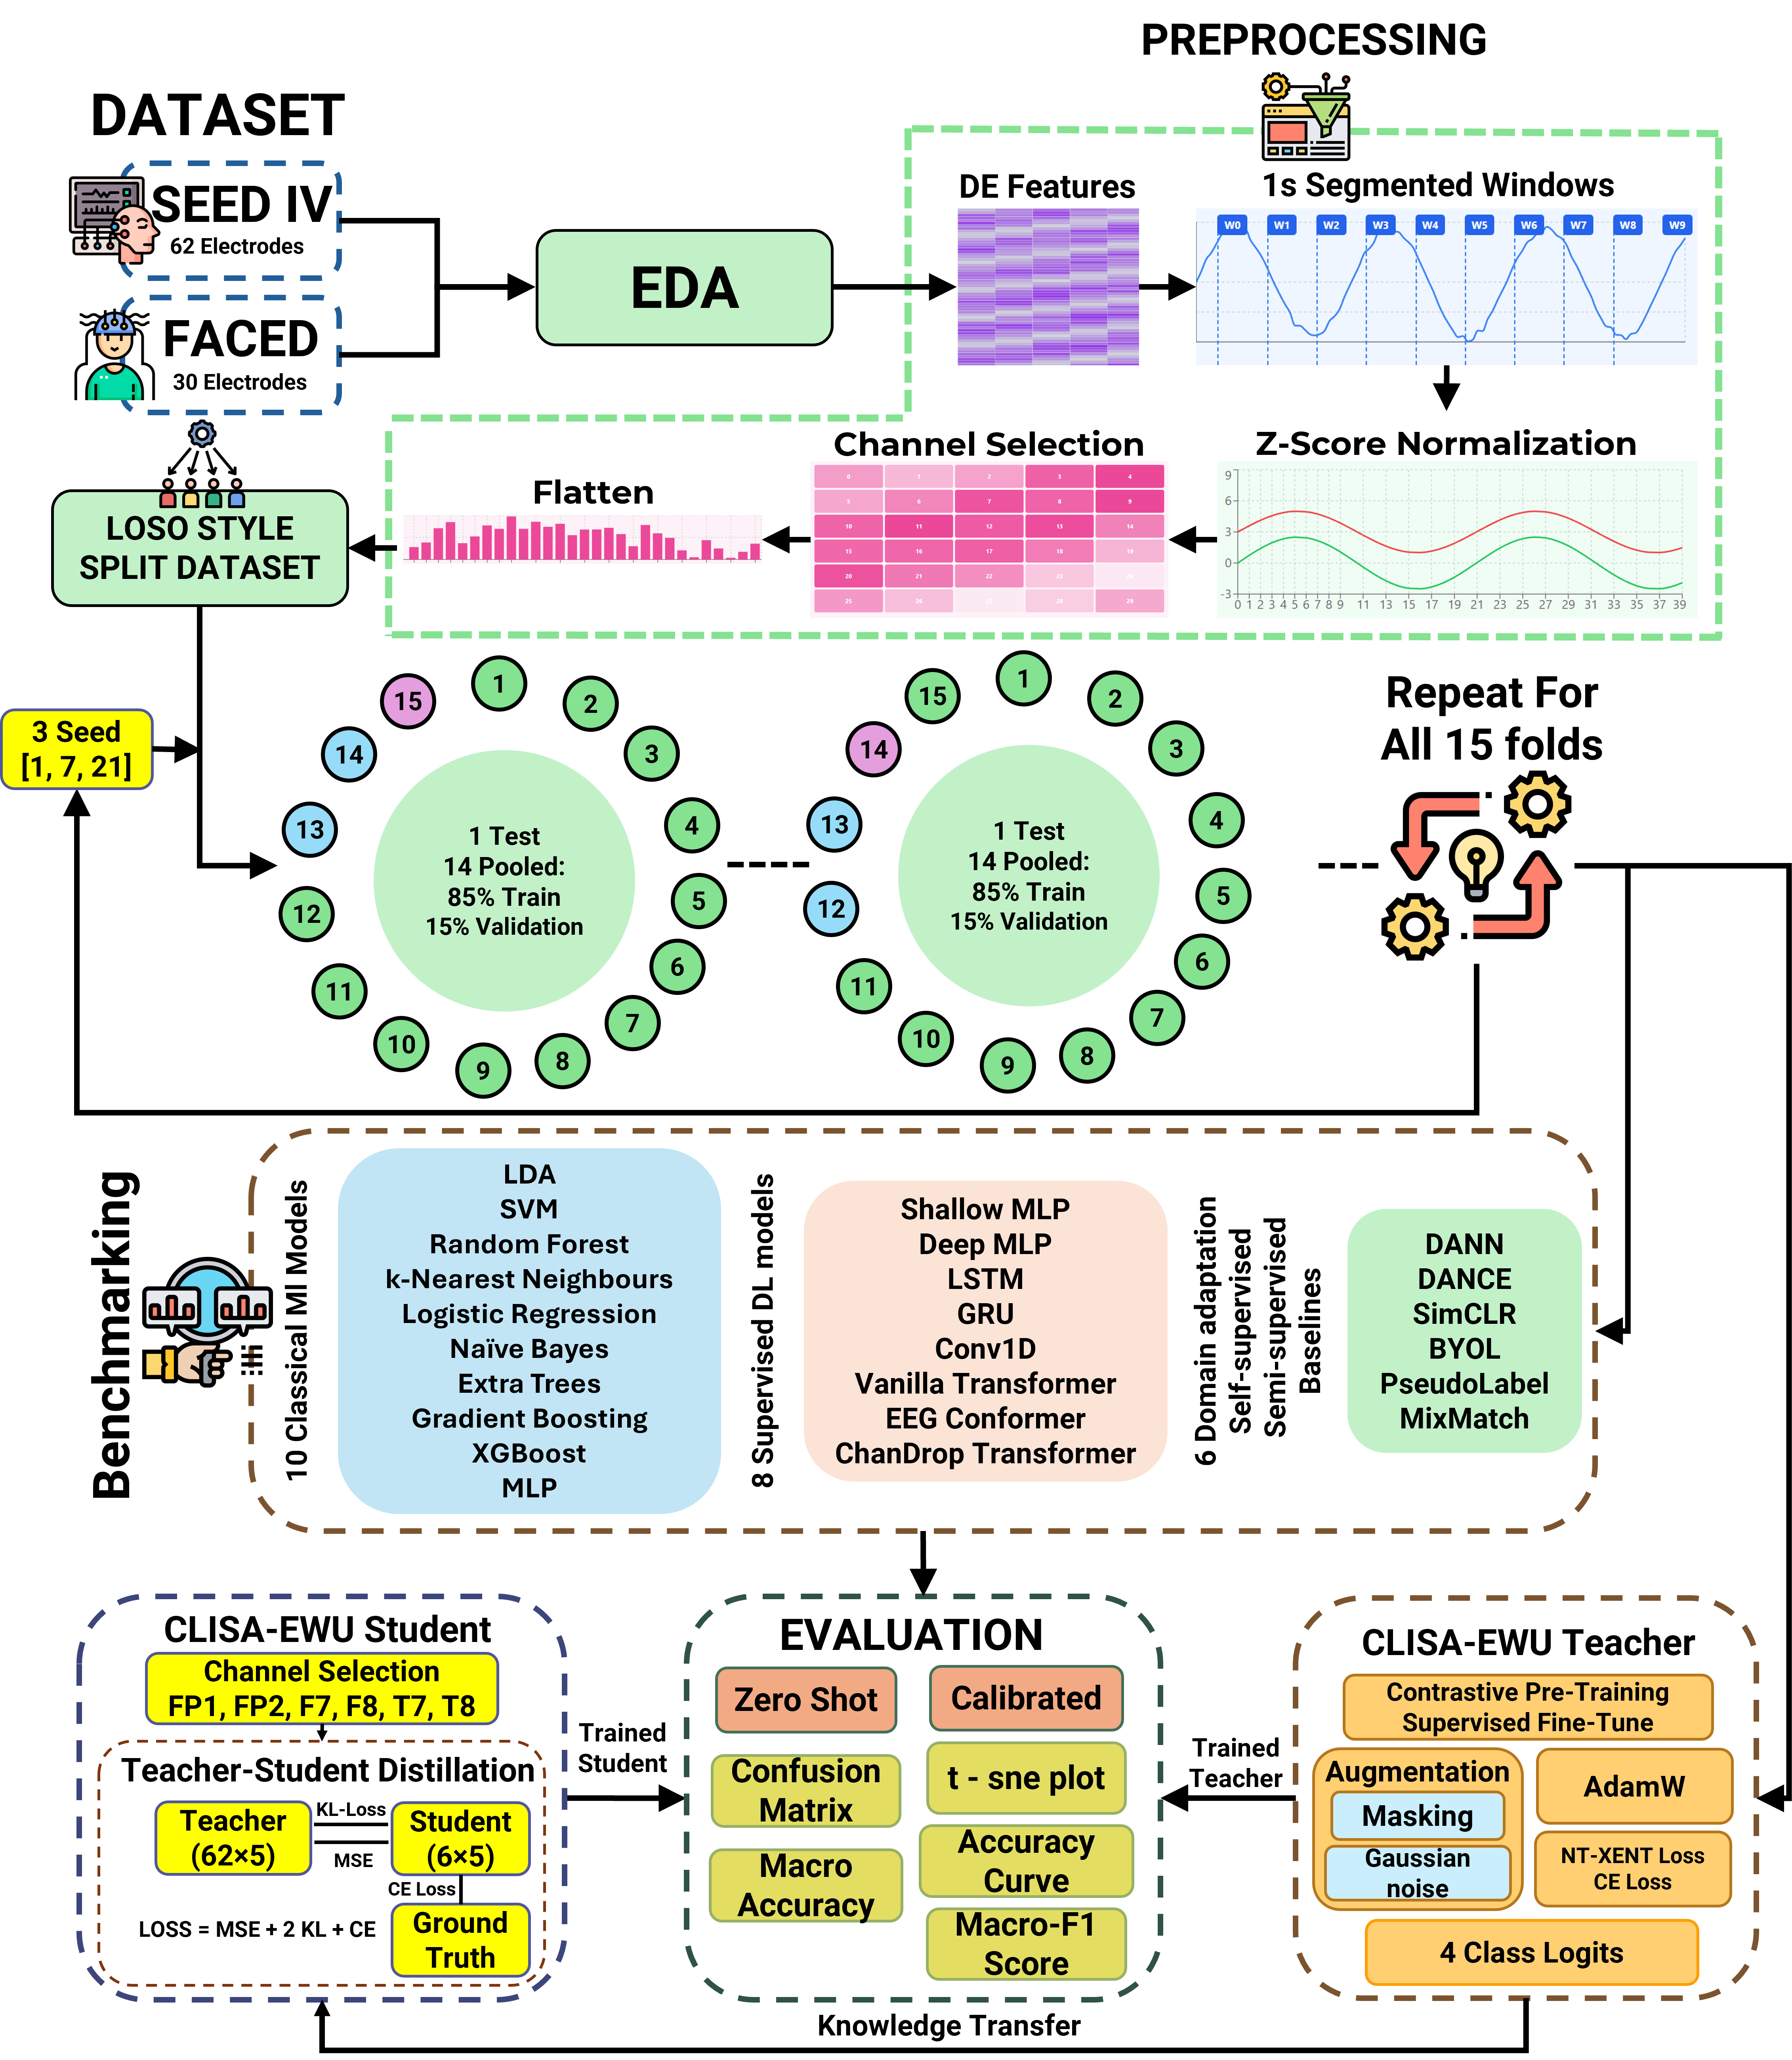
\includegraphics[width=0.82\linewidth,height=0.62\textheight,keepaspectratio]{figures/thesis_fig03_workflow.png}
  \caption{\textbf{Experimental workflow.} Exploratory data analysis; leave-one-participant-out splitting with three seeds; classical, supervised, self-supervised, semi-supervised and domain-adversarial model families; electrode selection for the six-electrode montage; and zero-shot and calibrated evaluation with accuracy, macro F1, confusion matrices and t-SNE.}
  \label{fig:workflow}
\end{figure}


\subsection{Dataset and features}
We analysed the public SEED-IV dataset\cite{seediv}. Fifteen healthy adults \pending{report sex and age range from the dataset paper} watched 72 film clips (24 per session, three sessions on different days) selected to elicit neutral, sad, fear and happy states while 62-channel EEG was recorded according to the international 10–20 system. The original study obtained ethics approval and informed consent; no new data were collected, and data access followed the dataset licence.

We used the differential-entropy features released with SEED-IV, computed in non-overlapping 4-s windows in five bands (delta, theta, alpha, beta, gamma) and smoothed with a linear dynamical system (de\_LDS)\cite{seed,seediv}. This yielded 37,575 windows (2505 per participant; neutral 10,170, sad 10,245, fear 9225, happy 7935; Fig.~\ref{fig:dataset}). The full montage gave 310 features per window (62 electrodes × 5 bands). The wearable-compatible montage used six electrodes reachable by a forehead-and-temple band (FP1, FP2, F7, F8, T7, T8; 30 features). It is an exact subset of the full feature matrix, so montage comparisons are not confounded by preprocessing. Features were z-standardised before modelling \pending{confirm that standardisation statistics are computed within each training fold; re-run if they were computed on all 15 participants}.

\begin{figure}[!htbp]
  \centering
  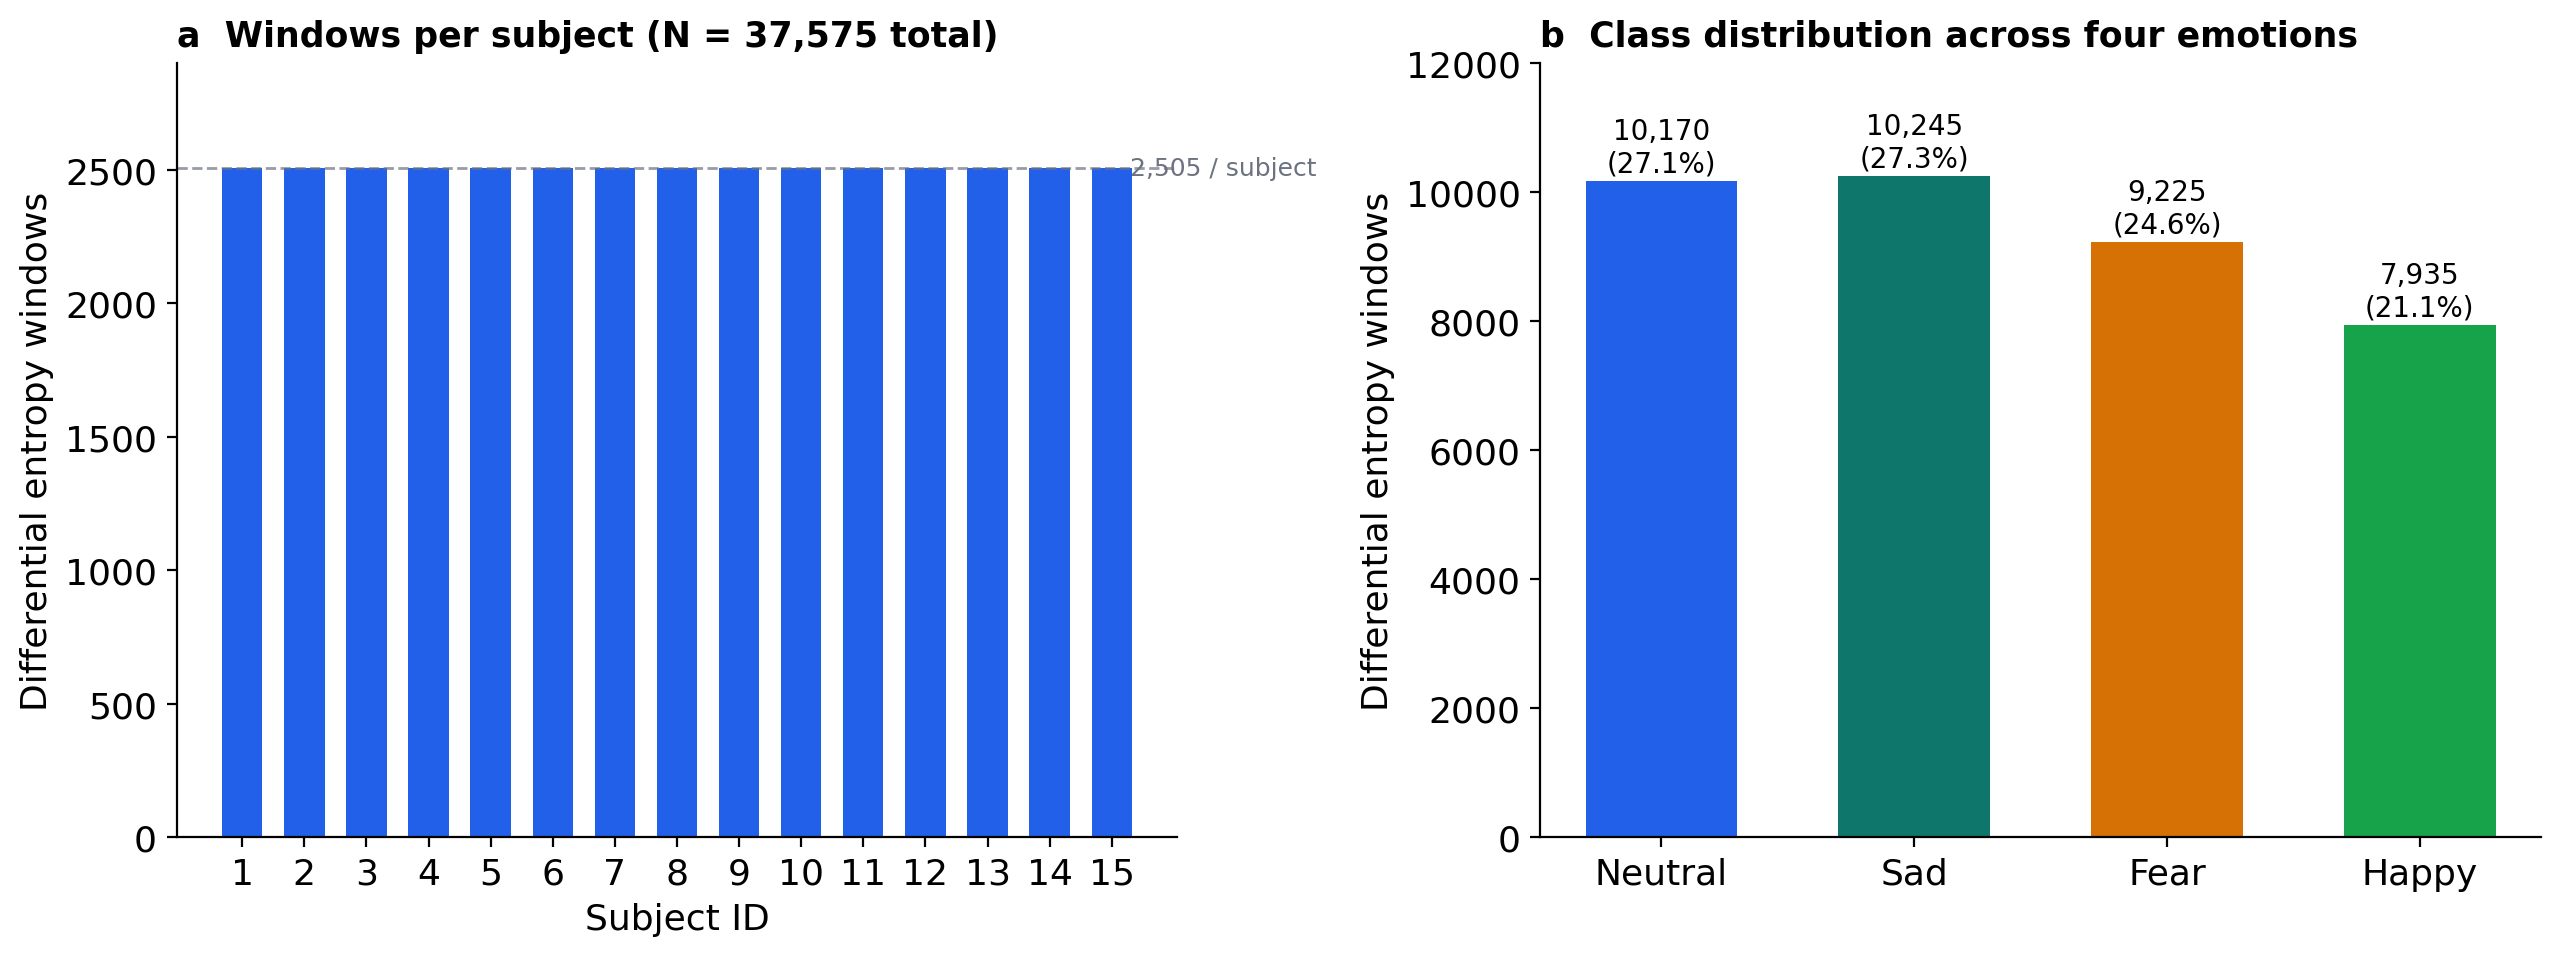
\includegraphics[width=1\linewidth,height=0.62\textheight,keepaspectratio]{figures/thesis_fig01_dataset_composition.png}
  \caption{\textbf{SEED-IV differential-entropy dataset composition.} (a) Windows per participant (2505 each; 37,575 in total). (b) Windows per emotion class.}
  \label{fig:dataset}
\end{figure}

This study used only the publicly available, de-identified SEED-IV dataset. Data collection was approved by the providers’ institutional ethics committee and all participants gave informed consent; no new human data were collected. All methods were carried out in accordance with relevant guidelines and regulations.


\subsection{Evaluation protocol}
We used leave-one-participant-out (LOSO) cross-validation. In each of 15 folds one participant was held out entirely, and the windows of the remaining 14 were split at random into training (85\%, about 29,810 windows) and validation (15\%, about 5260 windows) sets (Fig.~\ref{fig:split}). The procedure was repeated with seeds 1, 7 and 21, giving 45 runs per model and montage (Table~\ref{tab:protocol}). The complete workflow is shown in Fig.~\ref{fig:workflow}.

\begin{table}[!htbp]
  \centering
  {\small\setlength{\tabcolsep}{5pt}
  \begin{tabularx}{\linewidth}{@{}lX@{}}
  \toprule
\textbf{Item} & \textbf{Setting} \\
\midrule
Dataset & SEED-IV, 15 participants, 3 sessions, 72 trials per participant \\
Classes & Neutral, sad, fear, happy (four-class) \\
Features & Differential entropy (de\_LDS), 4-s windows, five bands \\
Full montage & 62 electrodes, 310 features \\
Wearable montage & FP1, FP2, F7, F8, T7, T8; 30 features \\
Split & Leave-one-participant-out, 15 folds; 85/15 random train/validation split of the 14 training participants \\
Seeds & 1, 7, 21 (45 runs per model and montage) \\
Protocols & Zero-shot; few-shot calibration with 20 labelled target windows \\
Metrics & Accuracy and macro F1 (all models); balanced accuracy, precision, specificity, weighted F1, Cohen’s κ, MCC, G-mean and ITR (CLISA-EWU and DANN) \\
Statistics & Participant-level means, bootstrap 95\% CI, paired Wilcoxon signed-rank tests, Holm correction \\
  \bottomrule
  \end{tabularx}}
  \caption{Dataset, feature and evaluation protocol summary.}
  \label{tab:protocol}
\end{table}

\begin{figure}[!htbp]
  \centering
  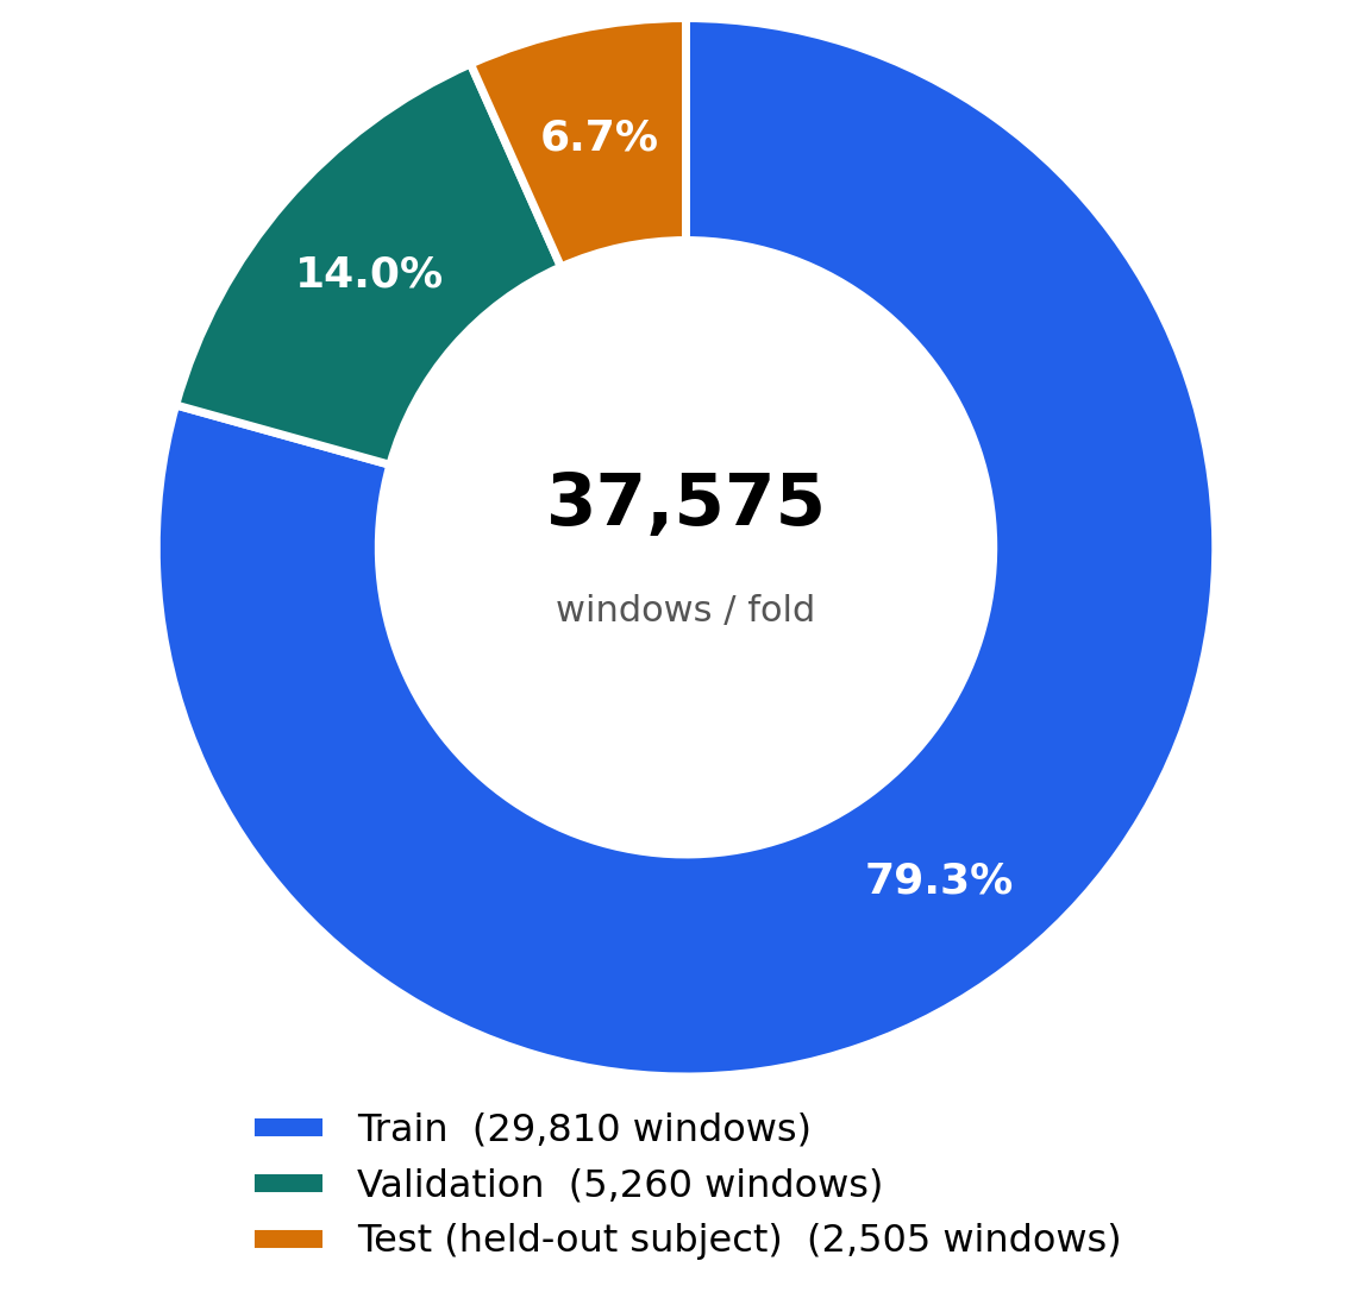
\includegraphics[width=0.82\linewidth,height=0.62\textheight,keepaspectratio]{figures/thesis_fig02_loso_split.png}
  \caption{\textbf{Composition of one leave-one-participant-out fold.} Windows of the 14 training participants were split at random into training (79.3\% of all windows) and validation (14.0\%) sets; all 2505 windows of the held-out participant (6.7\%) formed the test set. Validation windows share participants and trials with training windows.}
  \label{fig:split}
\end{figure}


\paragraph{Strategy 1: zero-shot evaluation}
The trained model predicts all 2505 windows of the held-out participant without access to any of their labels or unlabelled EEG (except for PseudoLabel, which uses unlabelled held-out EEG during training by design). This protocol measures true cross-participant generalization.


\paragraph{Strategy 2: few-shot calibration}
Twenty windows of the held-out participant are drawn at random, all network parameters are fine-tuned on them for 10 epochs (Adam, learning rate 10\textsuperscript{−3}), and performance is measured on the remaining 2485 windows. Twenty windows correspond to about 80 s of EEG, or 0.8\% of the participant’s data, and emulate a short user-calibration session.

Because calibration windows were sampled across trials, a calibration window and a test window could come from the same film-clip trial; with temporally smoothed features such windows are correlated, so calibrated estimates may be optimistic\cite{liblock} \pending{pending: trial-held-out calibration (calibrate on session 1, test on sessions 2–3) and a calibration-budget curve of 5–200 windows}. Validation windows came from the same participants and trials as training windows, so validation scores were near ceiling (median macro F1 1.00 for supervised models) and early stopping effectively selected late epochs; this does not compromise the independence of the held-out participant.


\subsection{Model families}
We evaluated ten classical classifiers (linear discriminant analysis, support vector machine with radial basis kernel, random forest, extra trees, gradient boosting, XGBoost\cite{xgboost}, k-nearest neighbours, logistic regression, naive Bayes and a scikit-learn multilayer perceptron) and 16 deep models in five families (Table~\ref{tab:models}): supervised networks (two-layer and deep perceptrons, LSTM, GRU, one-dimensional CNN, transformer\cite{vaswani}, EEG Conformer\cite{conformer} and a channel-dropout transformer); a domain-adversarial network (DANN)\cite{ganin} whose discriminator predicted training-participant identity through a gradient-reversal layer; self-supervised models (SimCLR\cite{simclr}, BYOL\cite{byol}); semi-supervised models (PseudoLabel\cite{pseudo}, which used confident predictions on the unlabelled held-out participant, and MixMatch\cite{mixmatch}); and a teacher–student distillation pair (DANCE)\cite{hinton}.

\begin{table}[!htbp]
  \centering
  {\small\setlength{\tabcolsep}{5pt}
  \begin{tabularx}{\linewidth}{@{}lXX@{}}
  \toprule
\textbf{Family} & \textbf{Models} & \textbf{Role} \\
\midrule
Classical machine learning & LDA, SVM, random forest, extra trees, gradient boosting, XGBoost, k-NN, logistic regression, naive Bayes, MLP (scikit-learn) & Non-deep baselines \\
Supervised deep learning & Two-layer perceptron, deep perceptron, LSTM, GRU, Conv1D, transformer, EEG Conformer, channel-dropout transformer & Supervised neural baselines \\
Domain-adversarial & DANN & Removes training-participant information \\
Self-supervised & SimCLR, BYOL & Contrastive and bootstrap pretraining \\
Semi-supervised & PseudoLabel (transductive), MixMatch & Exploits unlabelled data \\
Distillation & DANCE teacher (62) → student (6) & Secondary reference \\
Model of interest & CLISA-EWU & Two-stage contrastive pretraining and supervised fine-tuning \\
  \bottomrule
  \end{tabularx}}
  \caption{Model families evaluated in this study.}
  \label{tab:models}
\end{table}


\subsection{CLISA-EWU architecture}
CLISA-EWU (Fig.~\ref{fig:arch}) has an encoder of two fully connected layers (256 and 128 units, batch normalisation, ReLU, dropout 0.3), a two-layer projection head (64 units) and a linear classifier. In stage 1 (50 epochs), the encoder and projector were trained with the normalised temperature-scaled cross-entropy (NT-Xent) loss (temperature 0.5) on two views of each window: one with additive Gaussian noise (s.d. 0.1) and one with 30\% of electrodes masked across all bands. In stage 2 (up to 50 epochs), the whole network was fine-tuned with cross-entropy (AdamW, learning rate 3 × 10\textsuperscript{−4}, weight decay 10\textsuperscript{−4}, cosine schedule, class-balanced sampling, early stopping with patience 15 on validation macro F1). Unlike the original CLISA\cite{clisa}, which aligns time-locked responses of different participants to the same stimulus, the stage-1 objective contrasts augmented views of the same window and does not use participant or stimulus identity \pending{either implement cross-participant stimulus-aligned positives or rename the model to avoid implying explicit inter-subject alignment}. Hyperparameters for all models are given in the project repository together with the code \pending{add them as a supplementary table}.

\begin{figure}[!htbp]
  \centering
  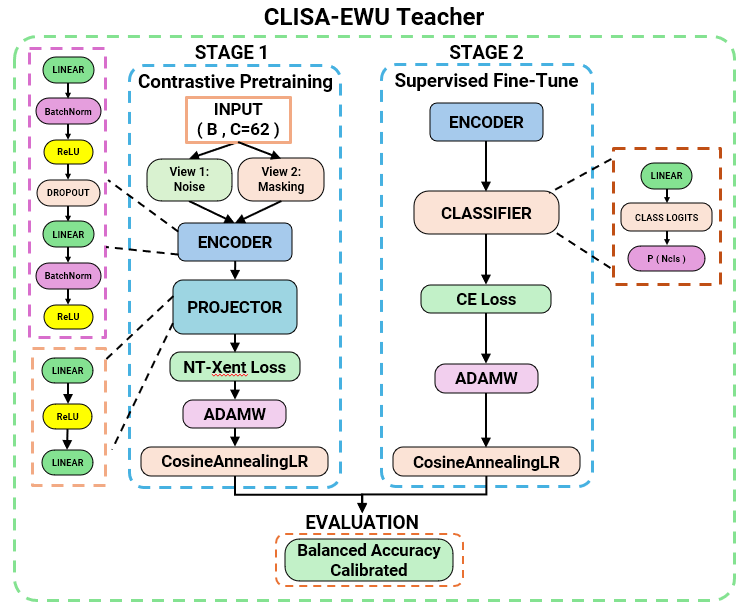
\includegraphics[width=1\linewidth,height=0.62\textheight,keepaspectratio]{figures/thesis_fig04_clisa_architecture.png}
  \caption{\textbf{CLISA-EWU architecture.} Stage 1: contrastive pretraining of the encoder and projector with the NT-Xent loss on a Gaussian-noise view and an electrode-masking view of each window (AdamW, cosine annealing). Stage 2: supervised fine-tuning of the encoder and linear classifier with cross-entropy. The model is evaluated zero-shot and after 20-window calibration.}
  \label{fig:arch}
\end{figure}

For a batch of \emph{N} windows, the two augmented views give 2\emph{N} projections \emph{z}. For a positive pair (\emph{i}, \emph{j}), the NT-Xent loss is

\begin{equation}
  \ell_{i,j} = -\log \frac{\exp\left(\mathrm{sim}(z_i,z_j)/\tau\right)}{\sum_{k=1,\,k\neq i}^{2N}\exp\left(\mathrm{sim}(z_i,z_k)/\tau\right)}
  \label{eq:ntxent}
\end{equation}
where sim(·,·) is cosine similarity and τ = 0.5 is the temperature; the loss is averaged over all positive pairs in the batch.


\paragraph{Training configuration}
Stage 1 uses AdamW (learning rate 10\textsuperscript{−3}, weight decay 10\textsuperscript{−4}, cosine annealing, 50 epochs, batch size 128). Stage 2 uses AdamW (learning rate 3 × 10\textsuperscript{−4}, weight decay 10\textsuperscript{−4}, cosine annealing, up to 50 epochs, early stopping with patience 15 on validation macro F1, class-balanced sampling). Supervised baselines were trained for up to 100 epochs with the same early-stopping rule. Mixed-precision training was used throughout.


\paragraph{Implementation}
All experiments were implemented in Python 3 with PyTorch \pending{version} (deep models), scikit-learn \pending{version} and XGBoost \pending{version} (classical models), and SciPy and statsmodels (statistics), and were run on an NVIDIA GeForce RTX 3050 Laptop GPU \pending{confirm hardware}.


\subsection{Evaluation metrics}
Model performance is assessed with complementary metrics computed on the test windows of the held-out participant. For class \emph{i} of \emph{C} = 4 classes, TP\textsubscript{i}, FP\textsubscript{i}, FN\textsubscript{i} and TN\textsubscript{i} denote true positives, false positives, false negatives and true negatives, \emph{n}\textsubscript{i} the number of windows of class \emph{i} and \emph{N} the total number of test windows. Accuracy, the metric logged for every run of all models, and per-class specificity are

\begin{equation}
  \mathrm{Accuracy}=\frac{1}{N}\sum_{i=1}^{C}TP_i,\qquad \mathrm{Specificity}_i=\frac{TN_i}{TN_i+FP_i}
  \label{eq:acc}
\end{equation}
Per-class recall (sensitivity) and precision are

\begin{equation}
  \mathrm{Recall}_i=\frac{TP_i}{TP_i+FN_i},\qquad \mathrm{Precision}_i=\frac{TP_i}{TP_i+FP_i}
  \label{eq:recall}
\end{equation}
Balanced accuracy (BA) is the mean per-class recall\cite{brodersen} and removes the influence of class frequency:

\begin{equation}
  \mathrm{BA}=\frac{1}{C}\sum_{i=1}^{C}\mathrm{Recall}_i
  \label{eq:bacc}
\end{equation}
The per-class F1 score is the harmonic mean of precision and recall; macro F1 averages it with equal class weights and weighted F1 with weights proportional to class support:

\begin{equation}
  F1_i=2\cdot\frac{\mathrm{Precision}_i\cdot\mathrm{Recall}_i}{\mathrm{Precision}_i+\mathrm{Recall}_i}
  \label{eq:f1}
\end{equation}
\begin{equation}
  F1_{\mathrm{macro}}=\frac{1}{C}\sum_{i=1}^{C}F1_i
  \label{eq:macrof1}
\end{equation}
\begin{equation}
  F1_{\mathrm{weighted}}=\sum_{i=1}^{C}\frac{n_i}{N}\,F1_i
  \label{eq:wf1}
\end{equation}
Cohen’s kappa\cite{cohen} corrects accuracy for the agreement expected by chance, where \emph{p}\textsubscript{o} is the observed accuracy and \emph{n}\textsubscript{i·} and \emph{n}\textsubscript{·i} are the row and column totals of the confusion matrix:

\begin{equation}
  \kappa=\frac{p_o-p_e}{1-p_e},\qquad p_e=\frac{1}{N^{2}}\sum_{i=1}^{C}n_{i\cdot}\,n_{\cdot i}
  \label{eq:kappa}
\end{equation}
The multi-class Matthews correlation coefficient\cite{gorodkin,chicco} uses every cell of the confusion matrix, with \emph{c} correctly classified windows and \emph{t}\textsubscript{i} and \emph{p}\textsubscript{i} the true and predicted totals of class \emph{i}; it ranges from −1 to 1, with 0 at chance:

\begin{equation}
  \mathrm{MCC}=\frac{c\,N-\sum_{i}p_i\,t_i}{\sqrt{\left(N^{2}-\sum_{i}p_i^{2}\right)\left(N^{2}-\sum_{i}t_i^{2}\right)}}
  \label{eq:mcc}
\end{equation}
The geometric mean of the recalls\cite{kubat} penalises a model that neglects any class:

\begin{equation}
  G=\Bigl(\prod_{i=1}^{C}\mathrm{Recall}_i\Bigr)^{1/C}
  \label{eq:gmean}
\end{equation}
To express performance in brain–computer-interface terms, the information transfer rate\cite{wolpaw} is computed from accuracy \emph{P} with window length \emph{T} = 4 s, giving bits per window (\emph{B}) and bits per minute:

\begin{equation}
  B=\log_2 C+P\log_2 P+(1-P)\log_2\frac{1-P}{C-1},\qquad \mathrm{ITR}=B\cdot\frac{60}{T}
  \label{eq:itr}
\end{equation}
Electrode-reduction retention is the ratio of six-electrode to 62-electrode accuracy for the same model:

\begin{equation}
  \mathrm{Retention}=\frac{\mathrm{Acc}_{6}}{\mathrm{Acc}_{62}}
  \label{eq:retention}
\end{equation}
The run logs stored accuracy and macro F1 for every deep model, and full confusion matrices for CLISA-EWU and DANN. The complete metric set is therefore reported for these two models, and model-wide comparisons use accuracy and macro F1. Because the four classes are nearly balanced (21–27\% of windows), accuracy and balanced accuracy differed by 0.0–0.4 percentage points on average and by at most 2.4 points in any single run. Confusion matrices are row-normalised so that each row shows the recall of one true class.


\subsection{Statistical analysis}
Runs from the same participant are not independent, so the three seeds were averaged for each participant, giving 15 paired observations per model, montage and protocol. Participant-level means are reported with 95\% confidence intervals from 10,000 bootstrap resamples of participants.

Differences among all models within a montage and protocol were tested with the Friedman test\cite{friedman} on participant-level accuracy, with Kendall’s \emph{W} as the effect size. Average ranks $\bar{R}$\textsubscript{j} of \emph{k} models over \emph{n} = 15 participants were compared with the Nemenyi critical difference\cite{demsar}, where \emph{q}\textsubscript{α} is the studentised range statistic divided by √2 at α = 0.05:

\begin{equation}
  \chi^{2}_{F}=\frac{12n}{k(k+1)}\Biggl[\sum_{j=1}^{k}\bar{R}_j^{2}-\frac{k(k+1)^{2}}{4}\Biggr],\qquad W=\frac{\chi^{2}_{F}}{n(k-1)}
  \label{eq:friedman}
\end{equation}
\begin{equation}
  \mathrm{CD}=q_{\alpha}\sqrt{\frac{k(k+1)}{6n}}
  \label{eq:cd}
\end{equation}
Pairwise comparisons of CLISA-EWU with seven comparators used two-sided Wilcoxon signed-rank tests\cite{wilcoxon} with Holm adjustment\cite{holm} over the 14 comparisons of each protocol, and paired \emph{t}-tests as a parametric check. Effect sizes were Cohen’s \emph{d}\textsubscript{z} for the paired differences \emph{D}\cite{lakens} and the matched-pairs rank-biserial correlation \emph{r}\textsubscript{rb}\cite{kerby}, where \emph{T}\textsuperscript{+} and \emph{T}\textsuperscript{−} are the sums of positive and negative signed ranks:

\begin{equation}
  d_z=\frac{\bar{D}}{s_D},\qquad r_{rb}=\frac{T^{+}-T^{-}}{T^{+}+T^{-}}
  \label{eq:effect}
\end{equation}
Variability of CLISA-EWU across participants and seeds was decomposed with a two-way analysis of variance without replication (participant × seed), and reliability across seeds was summarised with the consistency intraclass correlation\cite{shrout}, where MS\textsubscript{P} and MS\textsubscript{E} are the participant and residual mean squares and \emph{k} = 3 seeds:

\begin{equation}
  \mathrm{ICC}(3,1)=\frac{MS_P-MS_E}{MS_P+(k-1)\,MS_E}
  \label{eq:icc}
\end{equation}
Associations between zero-shot accuracy, calibration gain and montage were assessed with Spearman’s ρ. The 62- versus six-electrode difference was tested with the Wilcoxon test, and the confidence interval for retention was obtained by resampling participants. Analyses used Python 3 with SciPy and statsmodels, and the scripts are provided in the repository. Reporting follows TRIPOD+AI where applicable\cite{tripod}.


\subsection{Representation and attribution analysis}
Representation geometry was examined with t-SNE\cite{tsne} and with silhouette\cite{silhouette}, Davies–Bouldin\cite{dbi} and Calinski–Harabasz\cite{chi} indices computed on PCA-reduced raw features and on CLISA-EWU encoder embeddings, using emotion and participant labels. Electrode importance was estimated with gradient-based SHAP\cite{shap} on the 62-electrode model of the best run, summing absolute attributions over the five bands of each electrode separately for each predicted class.


\section{Results and discussion}
In this section, the results of the benchmark are presented. Zero-shot performance is reported first, followed by the effect of few-shot calibration, the paired statistical comparisons, electrode reduction, variability across participants, class-level behaviour, representation geometry and secondary analyses. The implications and limitations of the findings are discussed at the end of the section.


\subsection{Benchmark overview}
All 26 models completed 45 runs per montage. The best classical classifier reached an accuracy of 0.484 (XGBoost) with 62 electrodes and 0.441 (LDA) with six electrodes (Fig.~\ref{fig:classical}), confirming that differential-entropy features carry emotion information in unseen participants. Fig.~\ref{fig:leader} shows the calibrated leaderboard for all deep models, and Table~\ref{tab:results} summarises zero-shot and calibrated results for the main comparators.

\begin{table}[!htbp]
  \centering
  {\scriptsize\setlength{\tabcolsep}{2.6pt}
  \begin{tabular}{@{}lcccccccccc@{}}
  \toprule
\textbf{Model} & \textbf{Acc (ZS)} & \textbf{F1 (ZS)} & \textbf{Acc (Cal)} & \textbf{SD (Cal)} & \textbf{F1 (Cal)} & \textbf{Gain, points (95\% CI)} & \textbf{CV (\%)} & \textbf{Worst} & \textbf{Best} & \textbf{Rank} \\
\midrule
\multicolumn{11}{@{}l}{\textit{62 electrodes}} \\
CLISA-EWU & 0.485 & 0.479 & 0.678 & 0.078 & 0.673 & 19.3 (14.9, 23.8) & 11.5 & 0.541 & 0.813 & 1.40 \\
DANN & 0.458 & 0.455 & 0.662 & 0.080 & 0.654 & 20.4 (16.2, 24.5) & 12.0 & 0.528 & 0.800 & 2.40 \\
PseudoLabel & 0.468 & 0.466 & 0.657 & 0.072 & 0.654 & 18.9 (14.4, 23.7) & 10.9 & 0.538 & 0.766 & 2.53 \\
BYOL & 0.431 & 0.423 & 0.609 & 0.074 & 0.594 & 17.8 (15.3, 20.2) & 12.2 & 0.476 & 0.718 & 4.07 \\
SimCLR & 0.410 & 0.405 & 0.575 & 0.078 & 0.557 & 16.4 (13.2, 19.5) & 13.6 & 0.461 & 0.692 & 5.80 \\
MixMatch & 0.285 & 0.243 & 0.535 & 0.087 & 0.522 & 25.0 (22.0, 28.0) & 16.3 & 0.380 & 0.692 & 7.33 \\
DANCE teacher & 0.419 & 0.408 & 0.519 & 0.080 & 0.503 & 10.0 (7.0, 13.2) & 15.4 & 0.409 & 0.677 & 8.20 \\
Two-layer perceptron & 0.476 & 0.474 & 0.496 & 0.096 & 0.493 & 2.0 (0.9, 3.1) & 19.4 & 0.305 & 0.710 & 8.33 \\
Deep perceptron & 0.479 & 0.476 & 0.492 & 0.100 & 0.489 & 1.3 (0.3, 2.4) & 20.3 & 0.306 & 0.704 & 8.67 \\
EEG Conformer & 0.453 & 0.447 & 0.459 & 0.109 & 0.454 & 0.7 (−0.0, 1.5) & 23.8 & 0.248 & 0.635 & 10.53 \\
Conv1D & 0.430 & 0.419 & 0.445 & 0.103 & 0.438 & 1.5 (0.5, 2.7) & 23.2 & 0.291 & 0.677 & 11.57 \\
GRU & 0.439 & 0.431 & 0.441 & 0.104 & 0.434 & 0.2 (0.1, 0.4) & 23.5 & 0.273 & 0.691 & 11.70 \\
ChanDrop transformer & 0.430 & 0.418 & 0.431 & 0.064 & 0.419 & 0.1 (0.1, 0.2) & 14.8 & 0.335 & 0.579 & 12.07 \\
LSTM & 0.430 & 0.420 & 0.431 & 0.116 & 0.421 & 0.1 (0.0, 0.3) & 26.9 & 0.268 & 0.695 & 12.40 \\
Transformer & 0.405 & 0.393 & 0.407 & 0.072 & 0.395 & 0.2 (0.1, 0.3) & 17.6 & 0.277 & 0.555 & 13.00 \\
\midrule
\multicolumn{11}{@{}l}{\textit{Six electrodes}} \\
CLISA-EWU & 0.405 & 0.398 & 0.620 & 0.060 & 0.611 & 21.4 (18.2, 25.2) & 9.7 & 0.518 & 0.719 & 2.67 \\
BYOL & 0.440 & 0.433 & 0.612 & 0.086 & 0.598 & 17.2 (14.0, 20.3) & 14.0 & 0.469 & 0.735 & 3.07 \\
PseudoLabel & 0.405 & 0.394 & 0.610 & 0.072 & 0.600 & 20.6 (17.5, 24.0) & 11.7 & 0.484 & 0.725 & 3.07 \\
SimCLR & 0.446 & 0.441 & 0.602 & 0.090 & 0.582 & 15.6 (13.0, 17.8) & 14.9 & 0.423 & 0.739 & 3.73 \\
DANN & 0.396 & 0.386 & 0.590 & 0.063 & 0.579 & 19.4 (16.5, 22.5) & 10.7 & 0.500 & 0.695 & 3.87 \\
DANCE student & 0.390 & 0.377 & 0.571 & 0.078 & 0.541 & 18.1 (14.9, 21.5) & 13.6 & 0.452 & 0.699 & 4.60 \\
Two-layer perceptron & 0.400 & 0.393 & 0.412 & 0.085 & 0.405 & 1.1 (0.3, 1.9) & 20.6 & 0.256 & 0.539 & 9.33 \\
ChanDrop transformer & 0.391 & 0.383 & 0.398 & 0.049 & 0.390 & 0.7 (0.4, 1.0) & 12.4 & 0.323 & 0.497 & 9.67 \\
Deep perceptron & 0.398 & 0.389 & 0.401 & 0.076 & 0.396 & 0.3 (−0.6, 1.2) & 18.9 & 0.254 & 0.516 & 10.00 \\
Transformer & 0.368 & 0.358 & 0.371 & 0.052 & 0.360 & 0.3 (0.1, 0.4) & 14.1 & 0.296 & 0.490 & 10.93 \\
LSTM & 0.384 & 0.376 & 0.385 & 0.066 & 0.377 & 0.1 (−0.1, 0.2) & 17.2 & 0.246 & 0.520 & 11.13 \\
Conv1D & 0.375 & 0.366 & 0.379 & 0.074 & 0.373 & 0.4 (−0.4, 1.1) & 19.6 & 0.232 & 0.522 & 11.47 \\
GRU & 0.376 & 0.369 & 0.378 & 0.073 & 0.371 & 0.2 (0.0, 0.4) & 19.4 & 0.269 & 0.532 & 11.73 \\
MixMatch & 0.270 & 0.226 & 0.364 & 0.038 & 0.334 & 9.4 (7.8, 11.1) & 10.4 & 0.312 & 0.431 & 12.07 \\
EEG Conformer & 0.353 & 0.344 & 0.361 & 0.065 & 0.353 & 0.8 (0.2, 1.4) & 18.1 & 0.263 & 0.481 & 12.67 \\
  \bottomrule
  \end{tabular}}
  \caption{Cross-participant four-class emotion recognition for all 15 deep models per montage, zero-shot (ZS) and after 20-window calibration (Cal). Values are means over 15 held-out participants (each averaged over three seeds). Gain = calibrated minus zero-shot accuracy in percentage points with 95\% bootstrap CI; CV = between-participant coefficient of variation of calibrated accuracy; worst/best = lowest/highest participant; rank = Friedman average rank after calibration (1 = best). Chance accuracy is 0.25.}
  \label{tab:results}
\end{table}

\begin{figure}[!htbp]
  \centering
  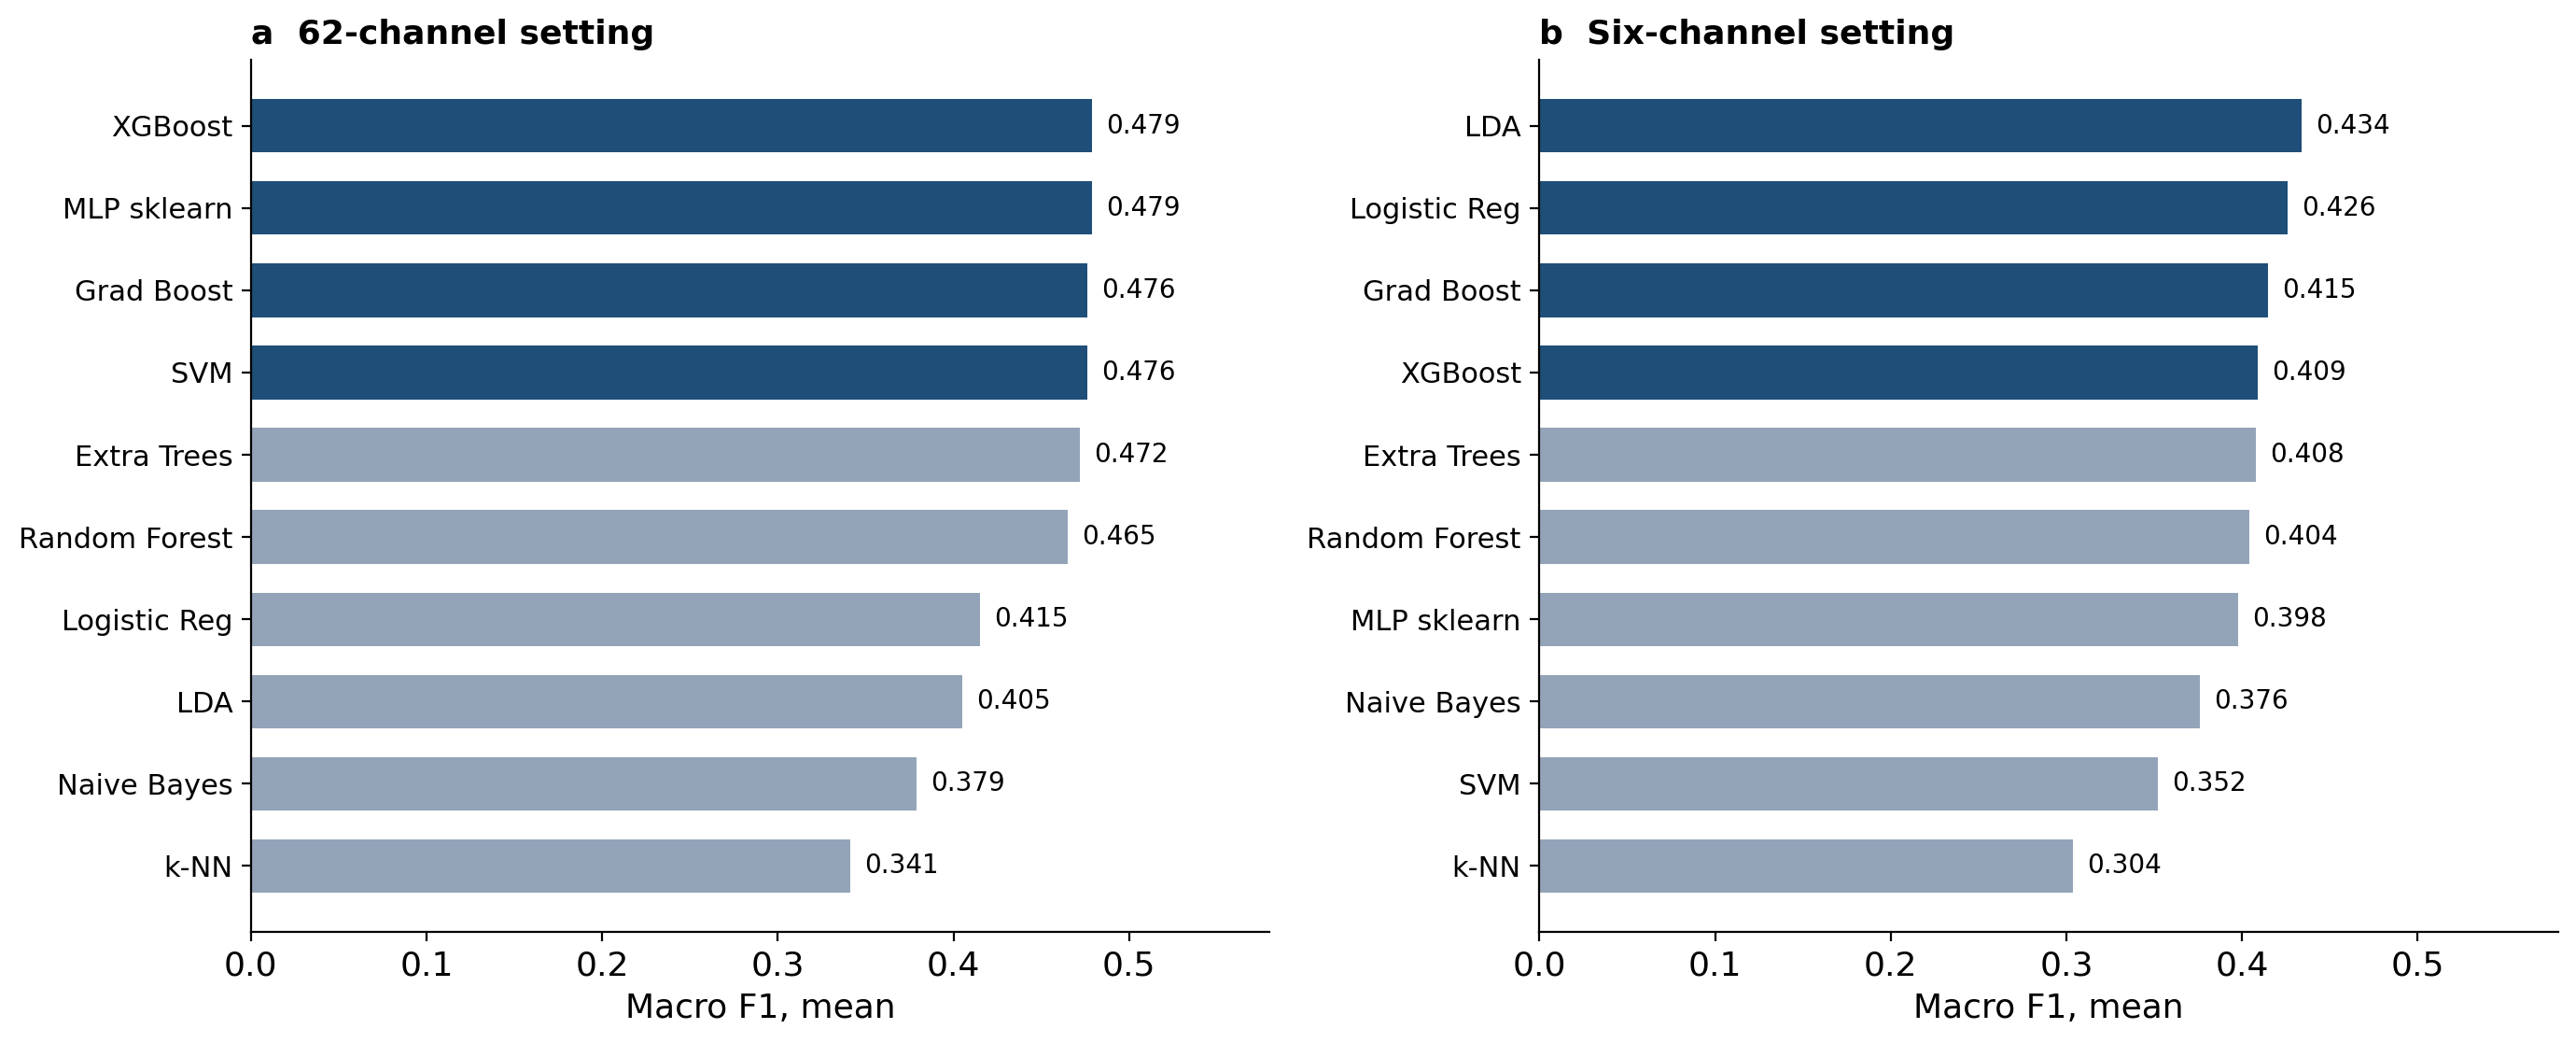
\includegraphics[width=1\linewidth,height=0.62\textheight,keepaspectratio]{figures/thesis_fig12_classical_leaderboards.png}
  \caption{\textbf{Classical machine-learning baselines.} Mean macro F1 over 45 leave-one-participant-out runs with (a) 62 electrodes and (b) six electrodes.}
  \label{fig:classical}
\end{figure}

\begin{figure}[!htbp]
  \centering
  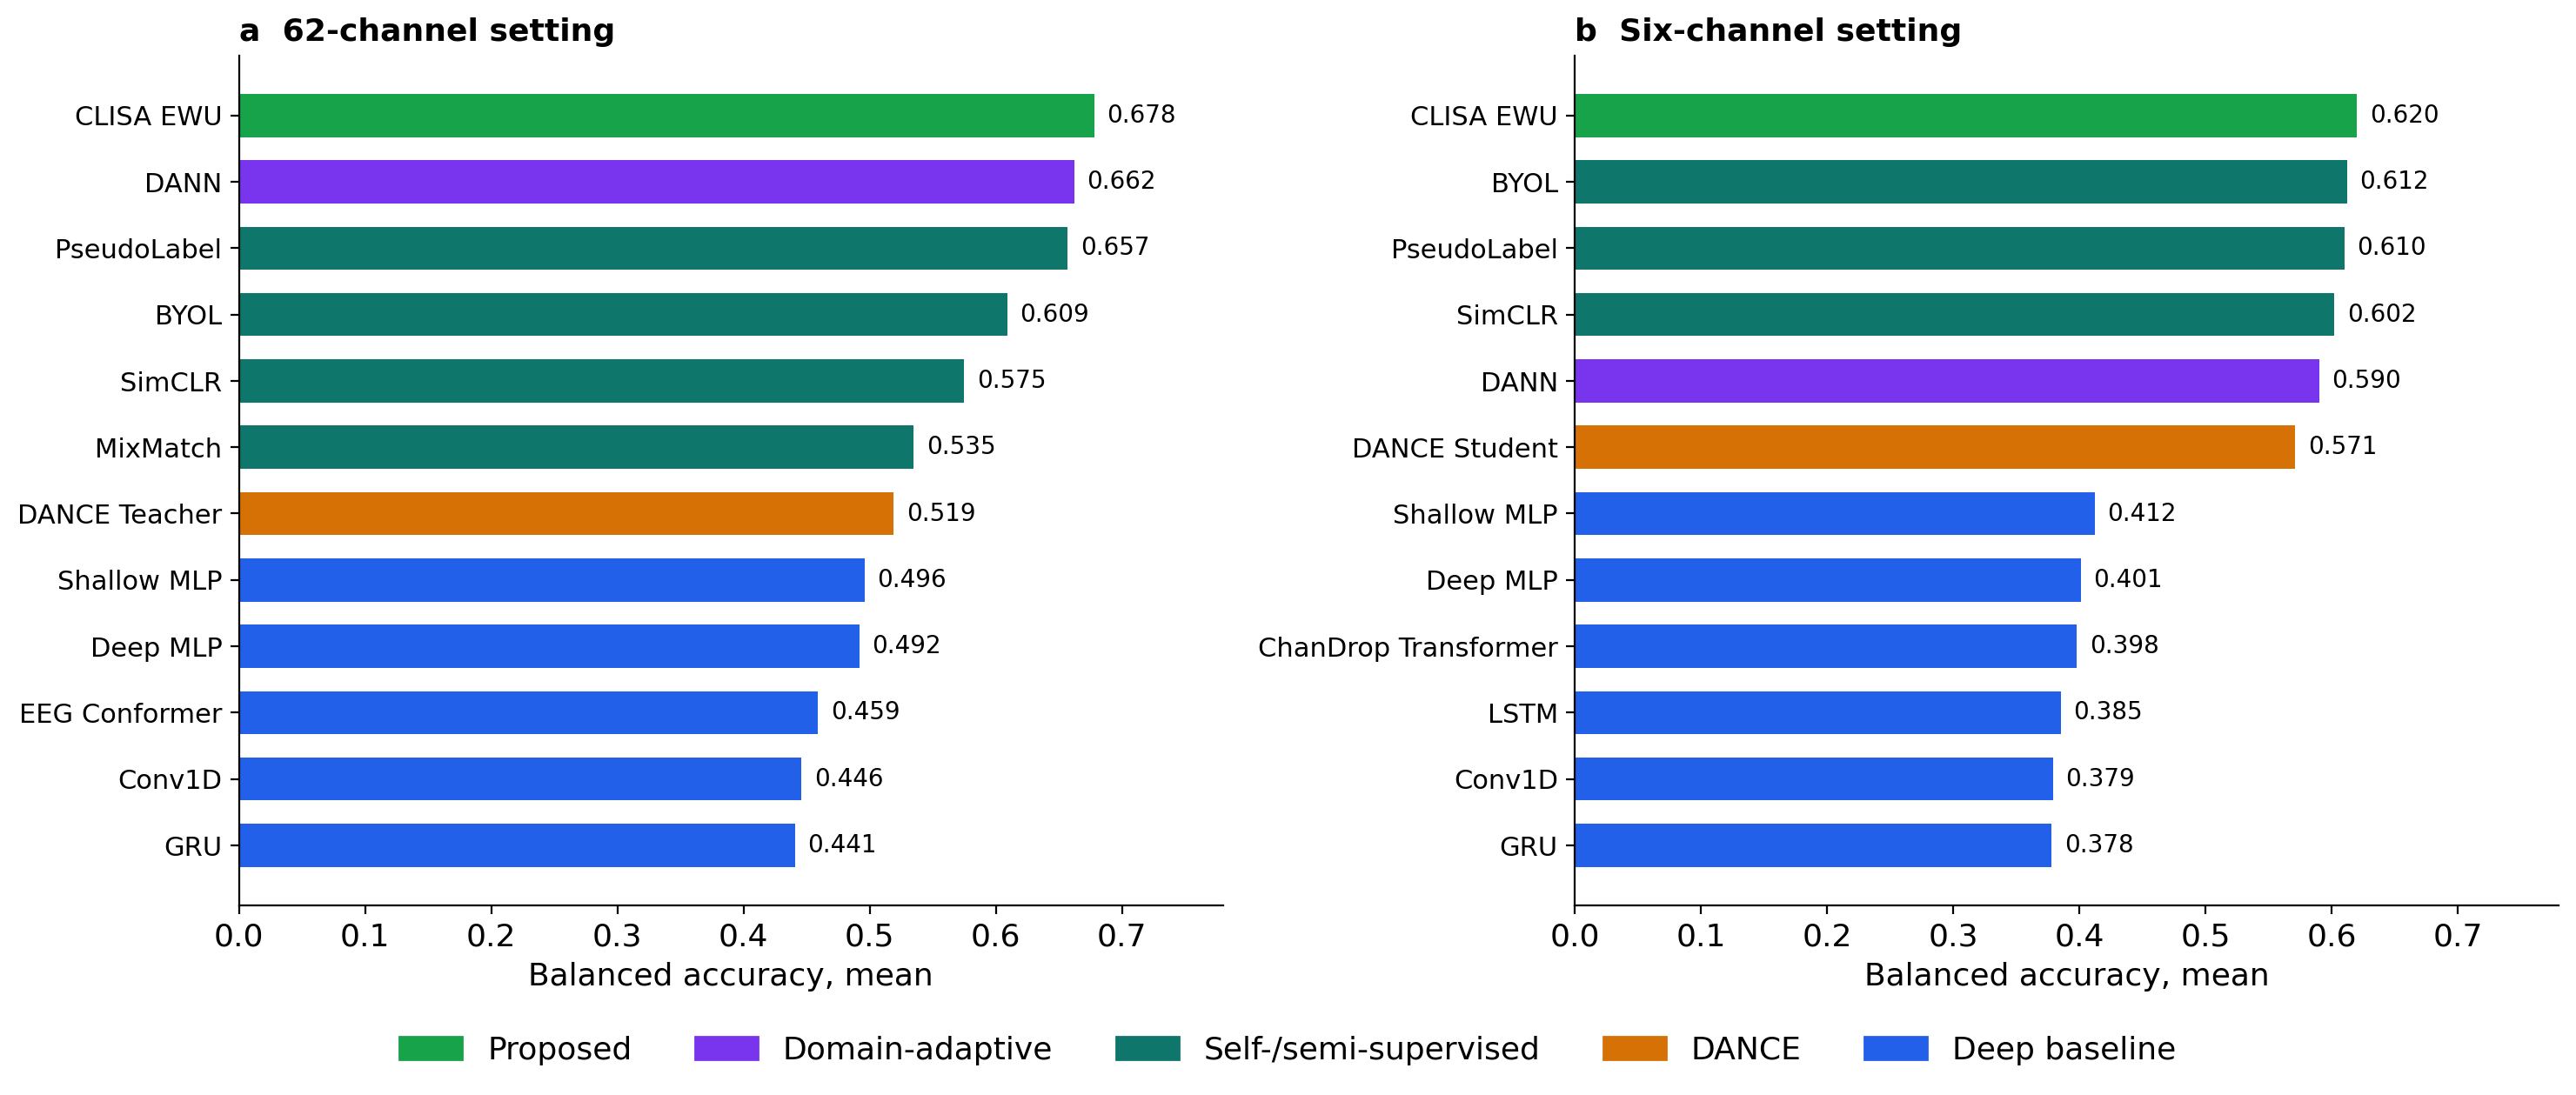
\includegraphics[width=1\linewidth,height=0.62\textheight,keepaspectratio]{figures/thesis_fig05_deep_leaderboards.png}
  \caption{\textbf{Calibrated performance of all deep models.} Mean accuracy over 45 runs after 20-window calibration with (a) 62 electrodes and (b) six electrodes. Colours denote model family (proposed, domain-adaptive, self/semi-supervised, DANCE, supervised baselines). Zero-shot results are shown in Fig.~\ref{fig:zs}. The axis label ‘balanced accuracy’ in this thesis figure denotes accuracy (see Methods).}
  \label{fig:leader}
\end{figure}


\subsection{Zero-shot cross-participant decoding}
Without target data, no model approached the accuracies reported in much of the literature (Fig.~\ref{fig:zs}). With 62 electrodes, CLISA-EWU had the highest mean zero-shot accuracy (0.485, 95\% CI 0.428–0.542) but did not differ from the two-layer perceptron (difference 0.9 percentage points, −0.5 to 2.1; Wilcoxon p = 0.25) or the deep perceptron (0.6 points, −0.9 to 2.2; p = 0.64). Its advantage over DANN (2.7 points, 1.0 to 4.2; unadjusted p = 0.010) did not survive Holm correction (p = 0.12). With six electrodes, zero-shot accuracy fell to 0.406 (0.370–0.439) for CLISA-EWU, and SimCLR (0.446) and BYOL (0.440) were numerically higher (both Holm-adjusted p = 1.00). Zero-shot performance varied greatly between participants, from 0.244 (participant 11, at chance) to 0.723 (participant 7) for CLISA-EWU with 62 electrodes (Fig.~\ref{fig:subj}a).

\begin{figure}[!htbp]
  \centering
  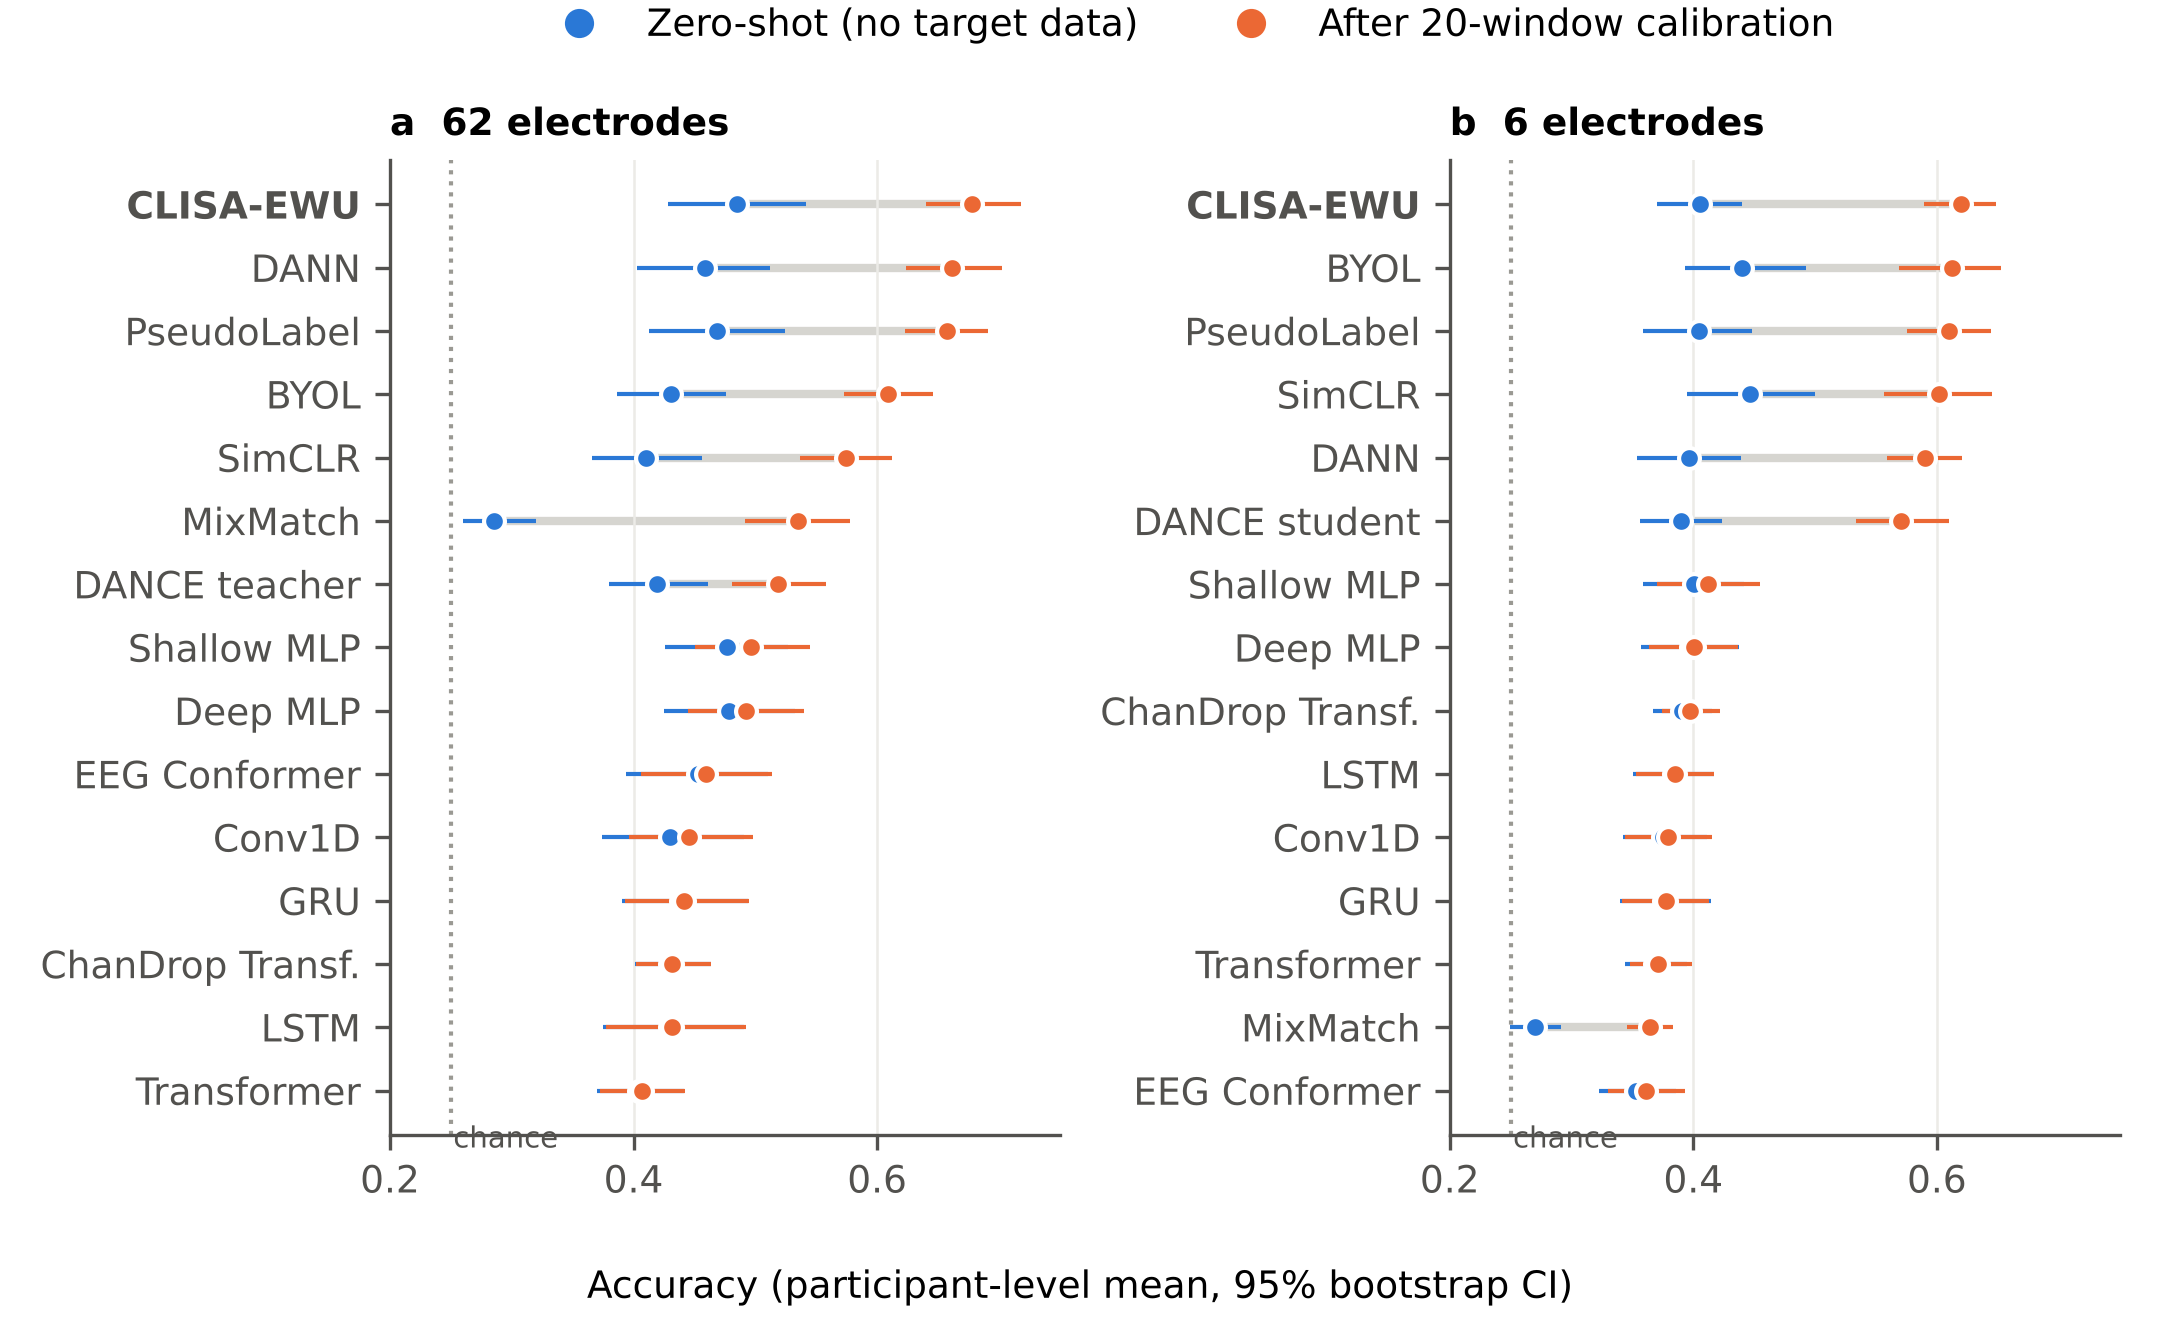
\includegraphics[width=1\linewidth,height=0.62\textheight,keepaspectratio]{figures/new_zeroshot_vs_calibrated.png}
  \caption{\textbf{Zero-shot versus calibrated accuracy for 16 deep models.} (a) 62 electrodes. (b) Six electrodes (FP1, FP2, F7, F8, T7, T8). Points are means over 15 held-out participants (each averaged over three seeds); bars are 95\% bootstrap confidence intervals; the grey segment joins the two protocols for each model. The dotted line marks chance (0.25).}
  \label{fig:zs}
\end{figure}

\begin{figure}[!htbp]
  \centering
  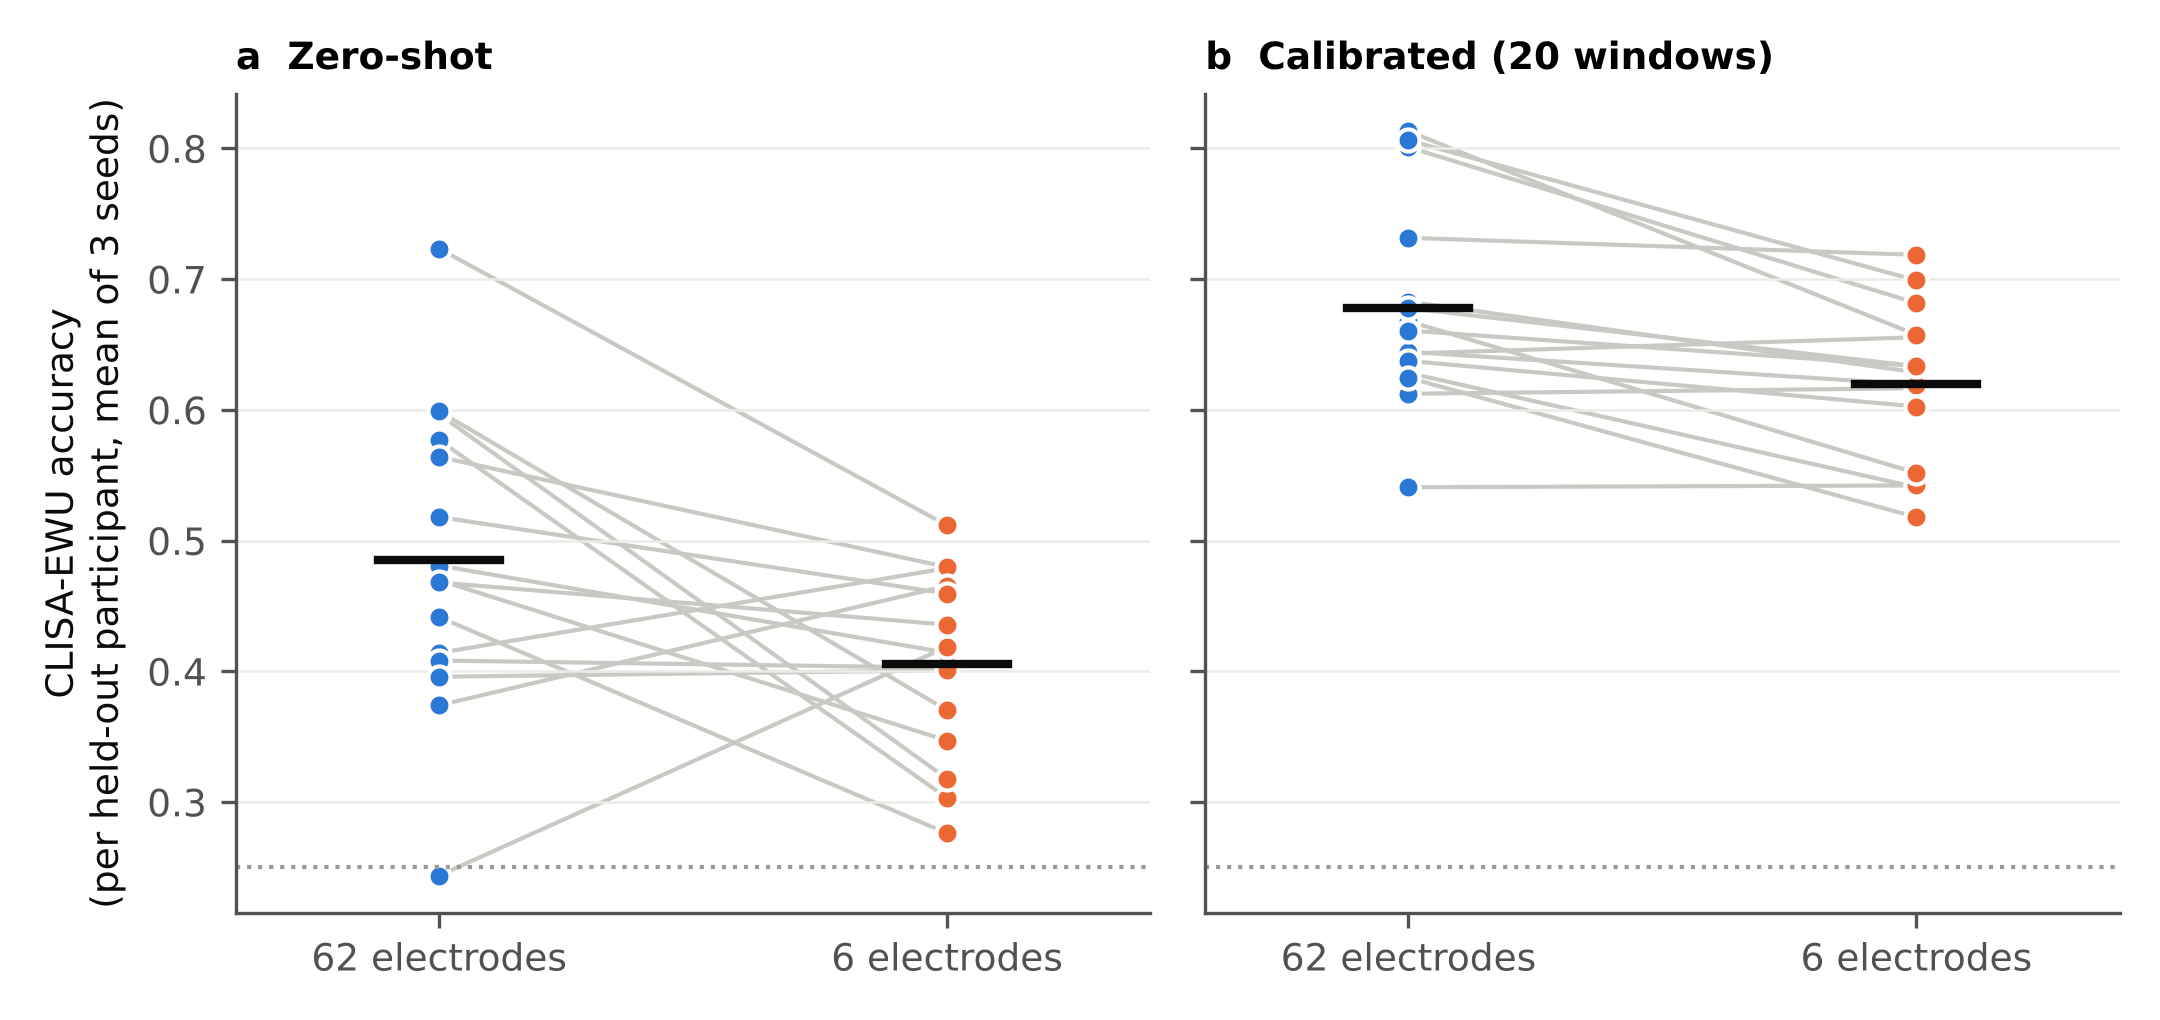
\includegraphics[width=1\linewidth,height=0.62\textheight,keepaspectratio]{figures/new_per_participant_montage.png}
  \caption{\textbf{Participant-level accuracy of CLISA-EWU with 62 and six electrodes.} (a) Zero-shot. (b) After 20-window calibration. Each line is one held-out participant (mean of three seeds); black bars are means over participants. The dotted line marks chance (0.25).}
  \label{fig:subj}
\end{figure}


\subsection{Effect of few-shot calibration}
Calibration with 20 labelled windows changed the ranking of models (Fig.~\ref{fig:zs}, Table~\ref{tab:results}). Models trained with a contrastive, domain-adversarial or pseudo-label objective (CLISA-EWU, SimCLR, BYOL, DANN, PseudoLabel) gained 15.6–21.4 percentage points (MixMatch and the DANCE pair gained 9.4–25.0 points), whereas purely supervised networks gained 0.1–2.0 points under the identical calibration routine. After calibration CLISA-EWU had the highest mean accuracy with both montages: 0.678 (0.641–0.718) with 62 electrodes and 0.620 (0.590–0.648) with six (Fig.~\ref{fig:violin}). The mechanism behind the objective-dependent gain is not established here; candidate explanations include adaptation of batch-normalisation statistics to the new participant\cite{adabn} and differences in how sharply each objective fits the training participants \pending{pending ablation: calibrate batch-normalisation statistics only, the classifier only, and all parameters}.

\begin{figure}[!htbp]
  \centering
  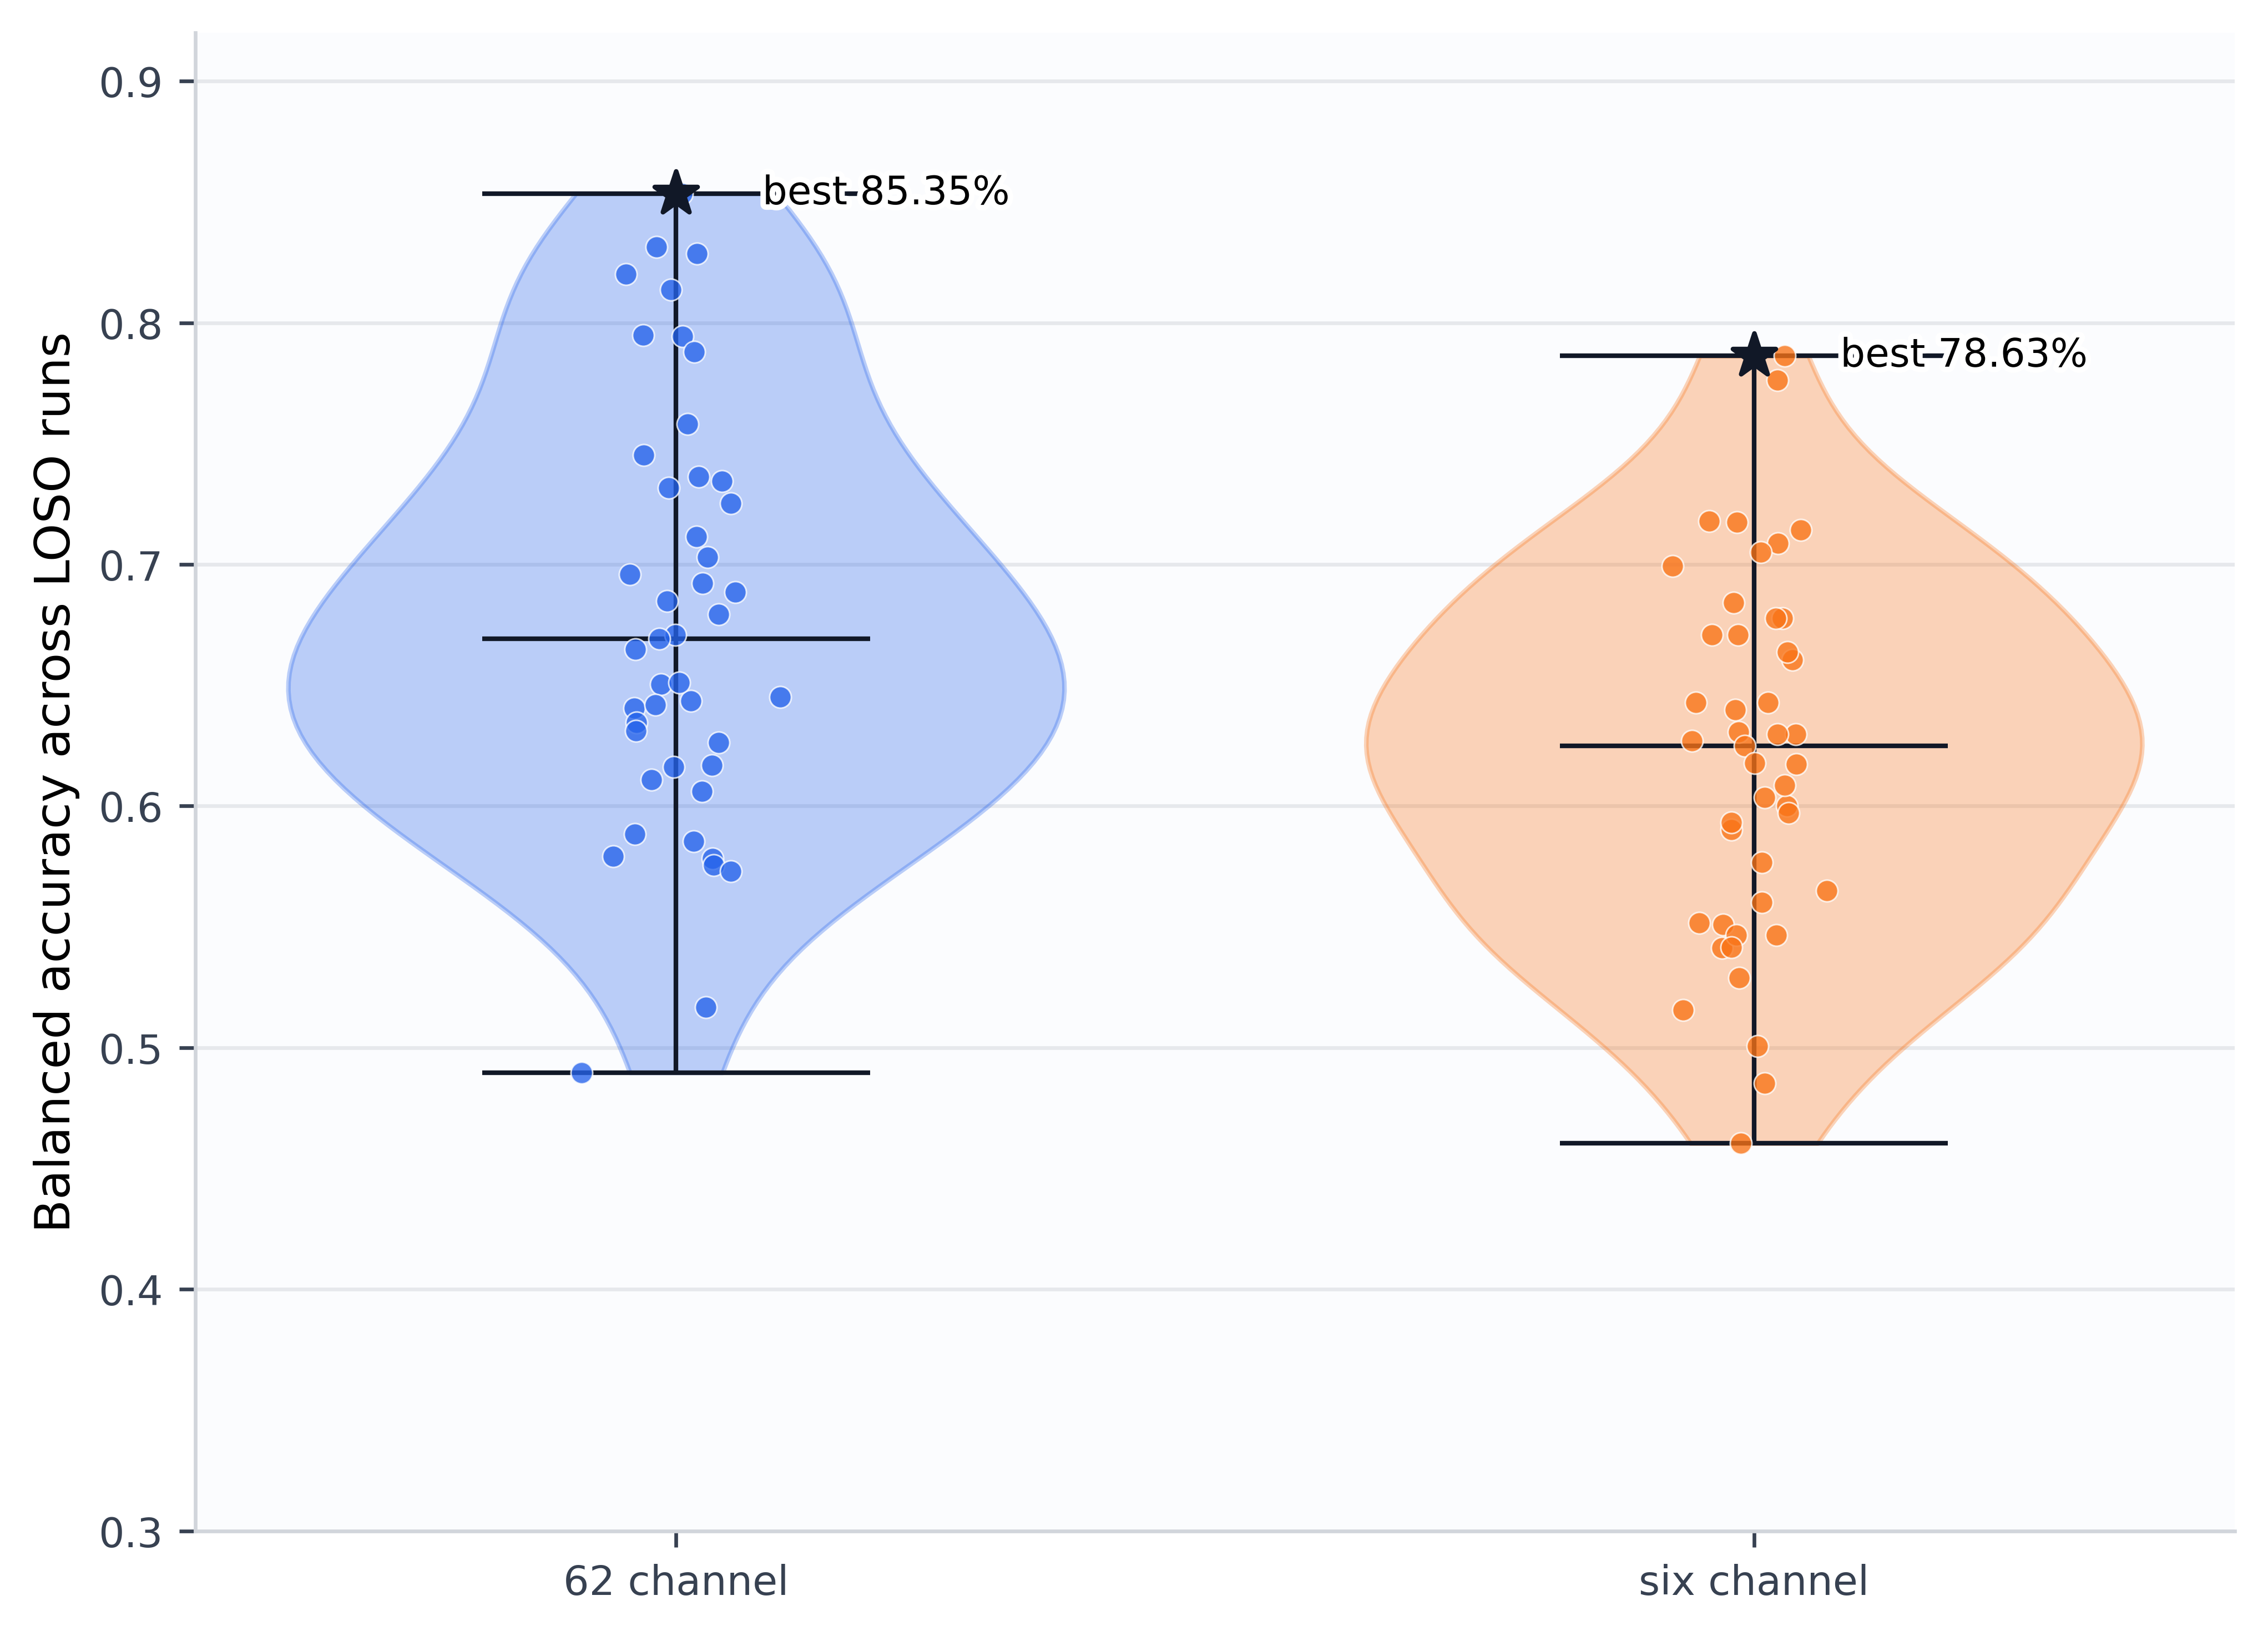
\includegraphics[width=1\linewidth,height=0.62\textheight,keepaspectratio]{figures/thesis_fig07_loso_distribution.png}
  \caption{\textbf{Run-level distribution of calibrated CLISA-EWU performance.} Accuracy for each of the 45 runs (15 held-out participants × 3 seeds) with 62 and six electrodes. Horizontal lines mark the mean and range; stars mark the best single runs (85.35\% and 78.63\%), shown for completeness and not as estimates of expected performance. The axis label ‘balanced accuracy’ in this thesis figure denotes accuracy (see Methods).}
  \label{fig:violin}
\end{figure}

In paired participant-level comparisons (Table~\ref{tab:paired}, Fig.~\ref{fig:pair}), calibrated CLISA-EWU outperformed BYOL (6.9 points, 5.2–8.5), SimCLR (10.3 points) and all supervised networks with 62 electrodes, for every one of the 15 participants. Its margin over PseudoLabel (2.1 points, 1.0–3.1; Holm p = 0.016) remained significant, but its margin over DANN (1.6 points, 0.6–2.6; Holm p = 0.062) did not. With six electrodes, CLISA-EWU, BYOL, PseudoLabel, SimCLR and DANN were statistically indistinguishable.

\begin{table}[!htbp]
  \centering
  {\footnotesize\setlength{\tabcolsep}{3.5pt}
  \begin{tabular}{@{}lccccccc@{}}
  \toprule
\textbf{Comparison} & \textbf{Δ, points (95\% CI)} & \textbf{d\textsubscript{z}} & \textbf{r\textsubscript{rb}} & \textbf{Wins} & \textbf{t-test p} & \textbf{Wilcoxon p} & \textbf{Holm p} \\
\midrule
\multicolumn{8}{@{}l}{\textit{Calibrated, 62 electrodes}} \\
vs DANN & 1.6 (0.7, 2.6) & 0.82 & 0.72 & 11/15 & 0.007 & 0.012 & 0.062 \\
vs PseudoLabel & 2.1 (1.0, 3.1) & 0.98 & 0.83 & 13/15 & 0.002 & 0.003 & 0.016 \\
vs BYOL & 6.9 (5.3, 8.6) & 2.04 & 1.00 & 15/15 & <0.001 & <0.001 & <0.001 \\
vs SimCLR & 10.3 (8.4, 12.3) & 2.62 & 1.00 & 15/15 & <0.001 & <0.001 & <0.001 \\
vs Two-layer perceptron & 18.2 (14.3, 22.0) & 2.33 & 1.00 & 15/15 & <0.001 & <0.001 & <0.001 \\
vs Deep perceptron & 18.6 (14.1, 22.9) & 2.07 & 1.00 & 15/15 & <0.001 & <0.001 & <0.001 \\
vs EEG Conformer & 21.9 (17.6, 26.4) & 2.42 & 1.00 & 15/15 & <0.001 & <0.001 & <0.001 \\
\midrule
\multicolumn{8}{@{}l}{\textit{Calibrated, six electrodes}} \\
vs DANN & 3.0 (0.9, 5.0) & 0.70 & 0.67 & 11/15 & 0.017 & 0.022 & 0.086 \\
vs PseudoLabel & 1.0 (−0.7, 2.7) & 0.28 & 0.30 & 9/15 & 0.300 & 0.330 & 0.688 \\
vs BYOL & 0.7 (−1.8, 3.4) & 0.14 & 0.13 & 8/15 & 0.591 & 0.679 & 0.688 \\
vs SimCLR & 1.8 (−1.2, 4.7) & 0.30 & 0.37 & 10/15 & 0.266 & 0.229 & 0.688 \\
vs Two-layer perceptron & 20.8 (17.0, 24.9) & 2.58 & 1.00 & 15/15 & <0.001 & <0.001 & <0.001 \\
vs Deep perceptron & 21.9 (18.6, 25.5) & 3.07 & 1.00 & 15/15 & <0.001 & <0.001 & <0.001 \\
vs EEG Conformer & 25.9 (22.6, 29.4) & 3.61 & 1.00 & 15/15 & <0.001 & <0.001 & <0.001 \\
\midrule
\multicolumn{8}{@{}l}{\textit{Zero-shot, 62 electrodes}} \\
vs DANN & 2.7 (1.0, 4.3) & 0.80 & 0.73 & 12/15 & 0.008 & 0.010 & 0.123 \\
vs PseudoLabel & 1.7 (−0.1, 3.5) & 0.46 & 0.43 & 8/15 & 0.099 & 0.151 & 1.000 \\
vs BYOL & 5.4 (1.1, 9.7) & 0.62 & 0.58 & 11/15 & 0.032 & 0.048 & 0.527 \\
vs SimCLR & 7.5 (2.8, 12.3) & 0.76 & 0.75 & 13/15 & 0.010 & 0.008 & 0.109 \\
vs Two-layer perceptron & 0.8 (−0.5, 2.1) & 0.31 & 0.35 & 10/15 & 0.243 & 0.252 & 1.000 \\
vs Deep perceptron & 0.6 (−0.9, 2.2) & 0.19 & 0.15 & 7/15 & 0.465 & 0.639 & 1.000 \\
vs EEG Conformer & 3.2 (−0.1, 6.7) & 0.45 & 0.45 & 9/15 & 0.102 & 0.135 & 1.000 \\
\midrule
\multicolumn{8}{@{}l}{\textit{Zero-shot, six electrodes}} \\
vs DANN & 0.9 (−1.4, 3.3) & 0.19 & 0.15 & 9/15 & 0.472 & 0.639 & 1.000 \\
vs PseudoLabel & 0.1 (−1.7, 1.9) & 0.02 & 0.03 & 8/15 & 0.936 & 0.934 & 1.000 \\
vs BYOL & −3.5 (−7.1, 0.2) & −0.46 & −0.45 & 5/15 & 0.096 & 0.135 & 1.000 \\
vs SimCLR & −4.1 (−8.7, 0.3) & −0.45 & −0.48 & 7/15 & 0.105 & 0.107 & 1.000 \\
vs Two-layer perceptron & 0.5 (−1.1, 2.3) & 0.14 & 0.03 & 6/15 & 0.597 & 0.934 & 1.000 \\
vs Deep perceptron & 0.8 (−0.9, 2.6) & 0.21 & 0.17 & 9/15 & 0.419 & 0.599 & 1.000 \\
vs EEG Conformer & 5.3 (3.5, 7.2) & 1.38 & 1.00 & 15/15 & <0.001 & <0.001 & <0.001 \\
  \bottomrule
  \end{tabular}}
  \caption{Paired participant-level comparisons of CLISA-EWU with other models. Δ = CLISA-EWU minus comparator in percentage points of accuracy (95\% bootstrap CI); d\textsubscript{z} = Cohen’s paired effect size; r\textsubscript{rb} = matched-pairs rank-biserial correlation; wins = participants favouring CLISA-EWU; p values from paired t-tests, Wilcoxon signed-rank tests and Holm adjustment (14 comparisons per protocol).}
  \label{tab:paired}
\end{table}

\begin{figure}[!htbp]
  \centering
  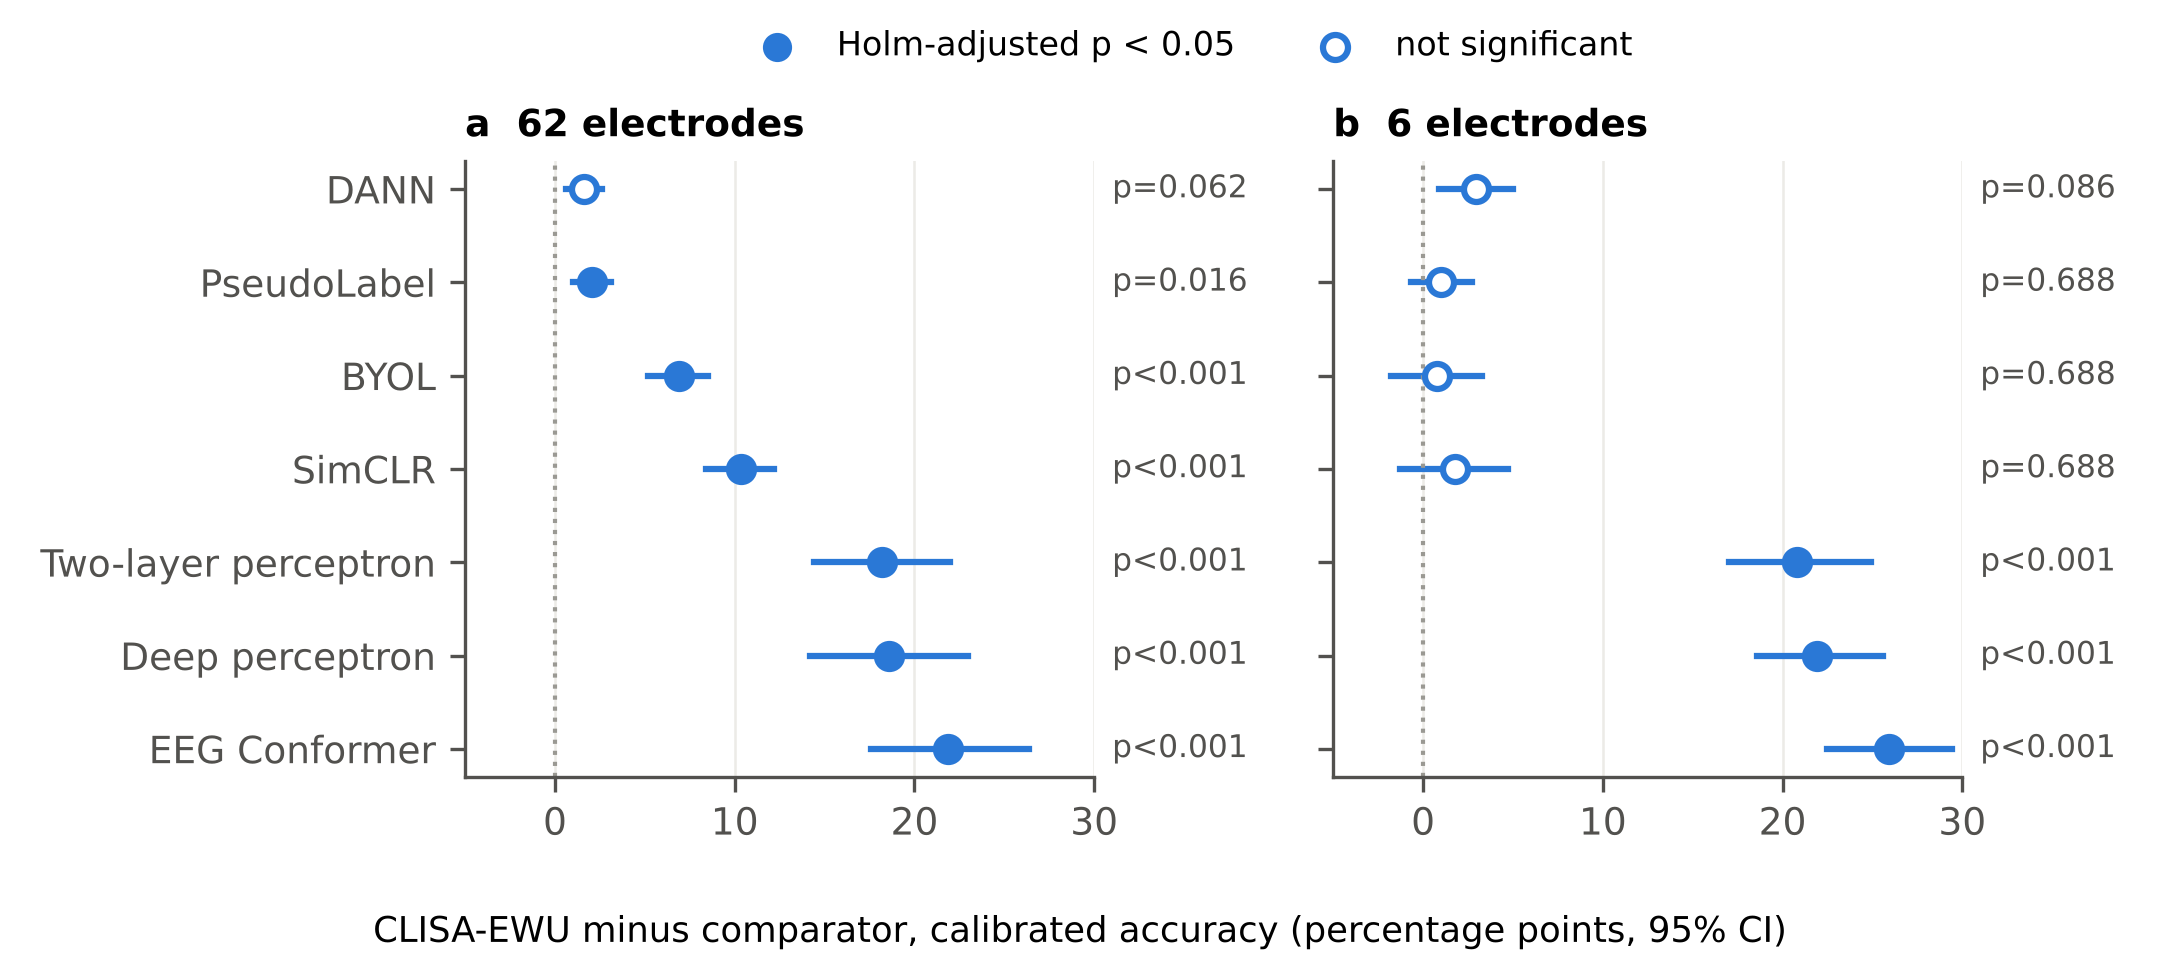
\includegraphics[width=1\linewidth,height=0.62\textheight,keepaspectratio]{figures/new_pairwise_wilcoxon.png}
  \caption{\textbf{Paired participant-level comparisons of calibrated CLISA-EWU with other models.} Differences in accuracy (CLISA-EWU minus comparator, percentage points) with 95\% bootstrap confidence intervals for (a) 62 and (b) six electrodes. Filled markers: Holm-adjusted Wilcoxon p < 0.05 (14 comparisons). This figure replaces a Welch t-test on run-level summaries, which treated 45 runs from 15 participants as independent.}
  \label{fig:pair}
\end{figure}


\subsection{Ranking across participants}
Friedman tests showed significant differences among the 15 deep models in every montage and protocol (Table~\ref{tab:friedman}; all p < 0.001). Agreement between participants on the ordering of models was weak zero-shot (Kendall’s W = 0.35 for both montages) but strong after calibration (W = 0.79 and 0.77), so calibration made the ranking consistent across people (Fig.~\ref{fig:cd}). After calibration, CLISA-EWU had the best average rank with 62 electrodes (1.40) and with six (2.67). The Nemenyi critical difference for 15 models and 15 participants was 5.54 ranks; by this conservative criterion, calibrated CLISA-EWU was distinguishable from every supervised network, MixMatch and the DANCE pair, but not from DANN (2.40), PseudoLabel (2.53), BYOL (4.07) or SimCLR (5.80) with 62 electrodes. Zero-shot, CLISA-EWU ranked first with 62 electrodes (4.53), but the deep and two-layer perceptrons were within 0.4 ranks of it, and with six electrodes it ranked third (5.93) behind BYOL (4.13) and SimCLR (4.87).

\begin{table}[!htbp]
  \centering
  {\footnotesize\setlength{\tabcolsep}{3.5pt}
  \begin{tabular}{@{}lccccccccc@{}}
  \toprule
\textbf{Ch} & \textbf{Protocol} & \textbf{k} & \textbf{n} & \textbf{χ²\textsubscript{F}} & \textbf{p} & \textbf{W} & \textbf{CD} & \textbf{Best model (rank)} & \textbf{CLISA-EWU rank} \\
\midrule
62 & Zero-shot & 15 & 15 & 72.6 & <0.001 & 0.35 & 5.54 & CLISA-EWU (4.53) & 4.53 \\
62 & Calibrated & 15 & 15 & 164.9 & <0.001 & 0.79 & 5.54 & CLISA-EWU (1.40) & 1.40 \\
6 & Zero-shot & 15 & 15 & 74.5 & <0.001 & 0.35 & 5.54 & BYOL (4.13) & 5.93 \\
6 & Calibrated & 15 & 15 & 161.4 & <0.001 & 0.77 & 5.54 & CLISA-EWU (2.67) & 2.67 \\
  \bottomrule
  \end{tabular}}
  \caption{Friedman tests across the 15 deep models of each montage (k models, n participants) with Kendall’s W, the Nemenyi critical difference (CD, α = 0.05), the best-ranked model and the average rank of CLISA-EWU.}
  \label{tab:friedman}
\end{table}

\begin{figure}[!htbp]
  \centering
  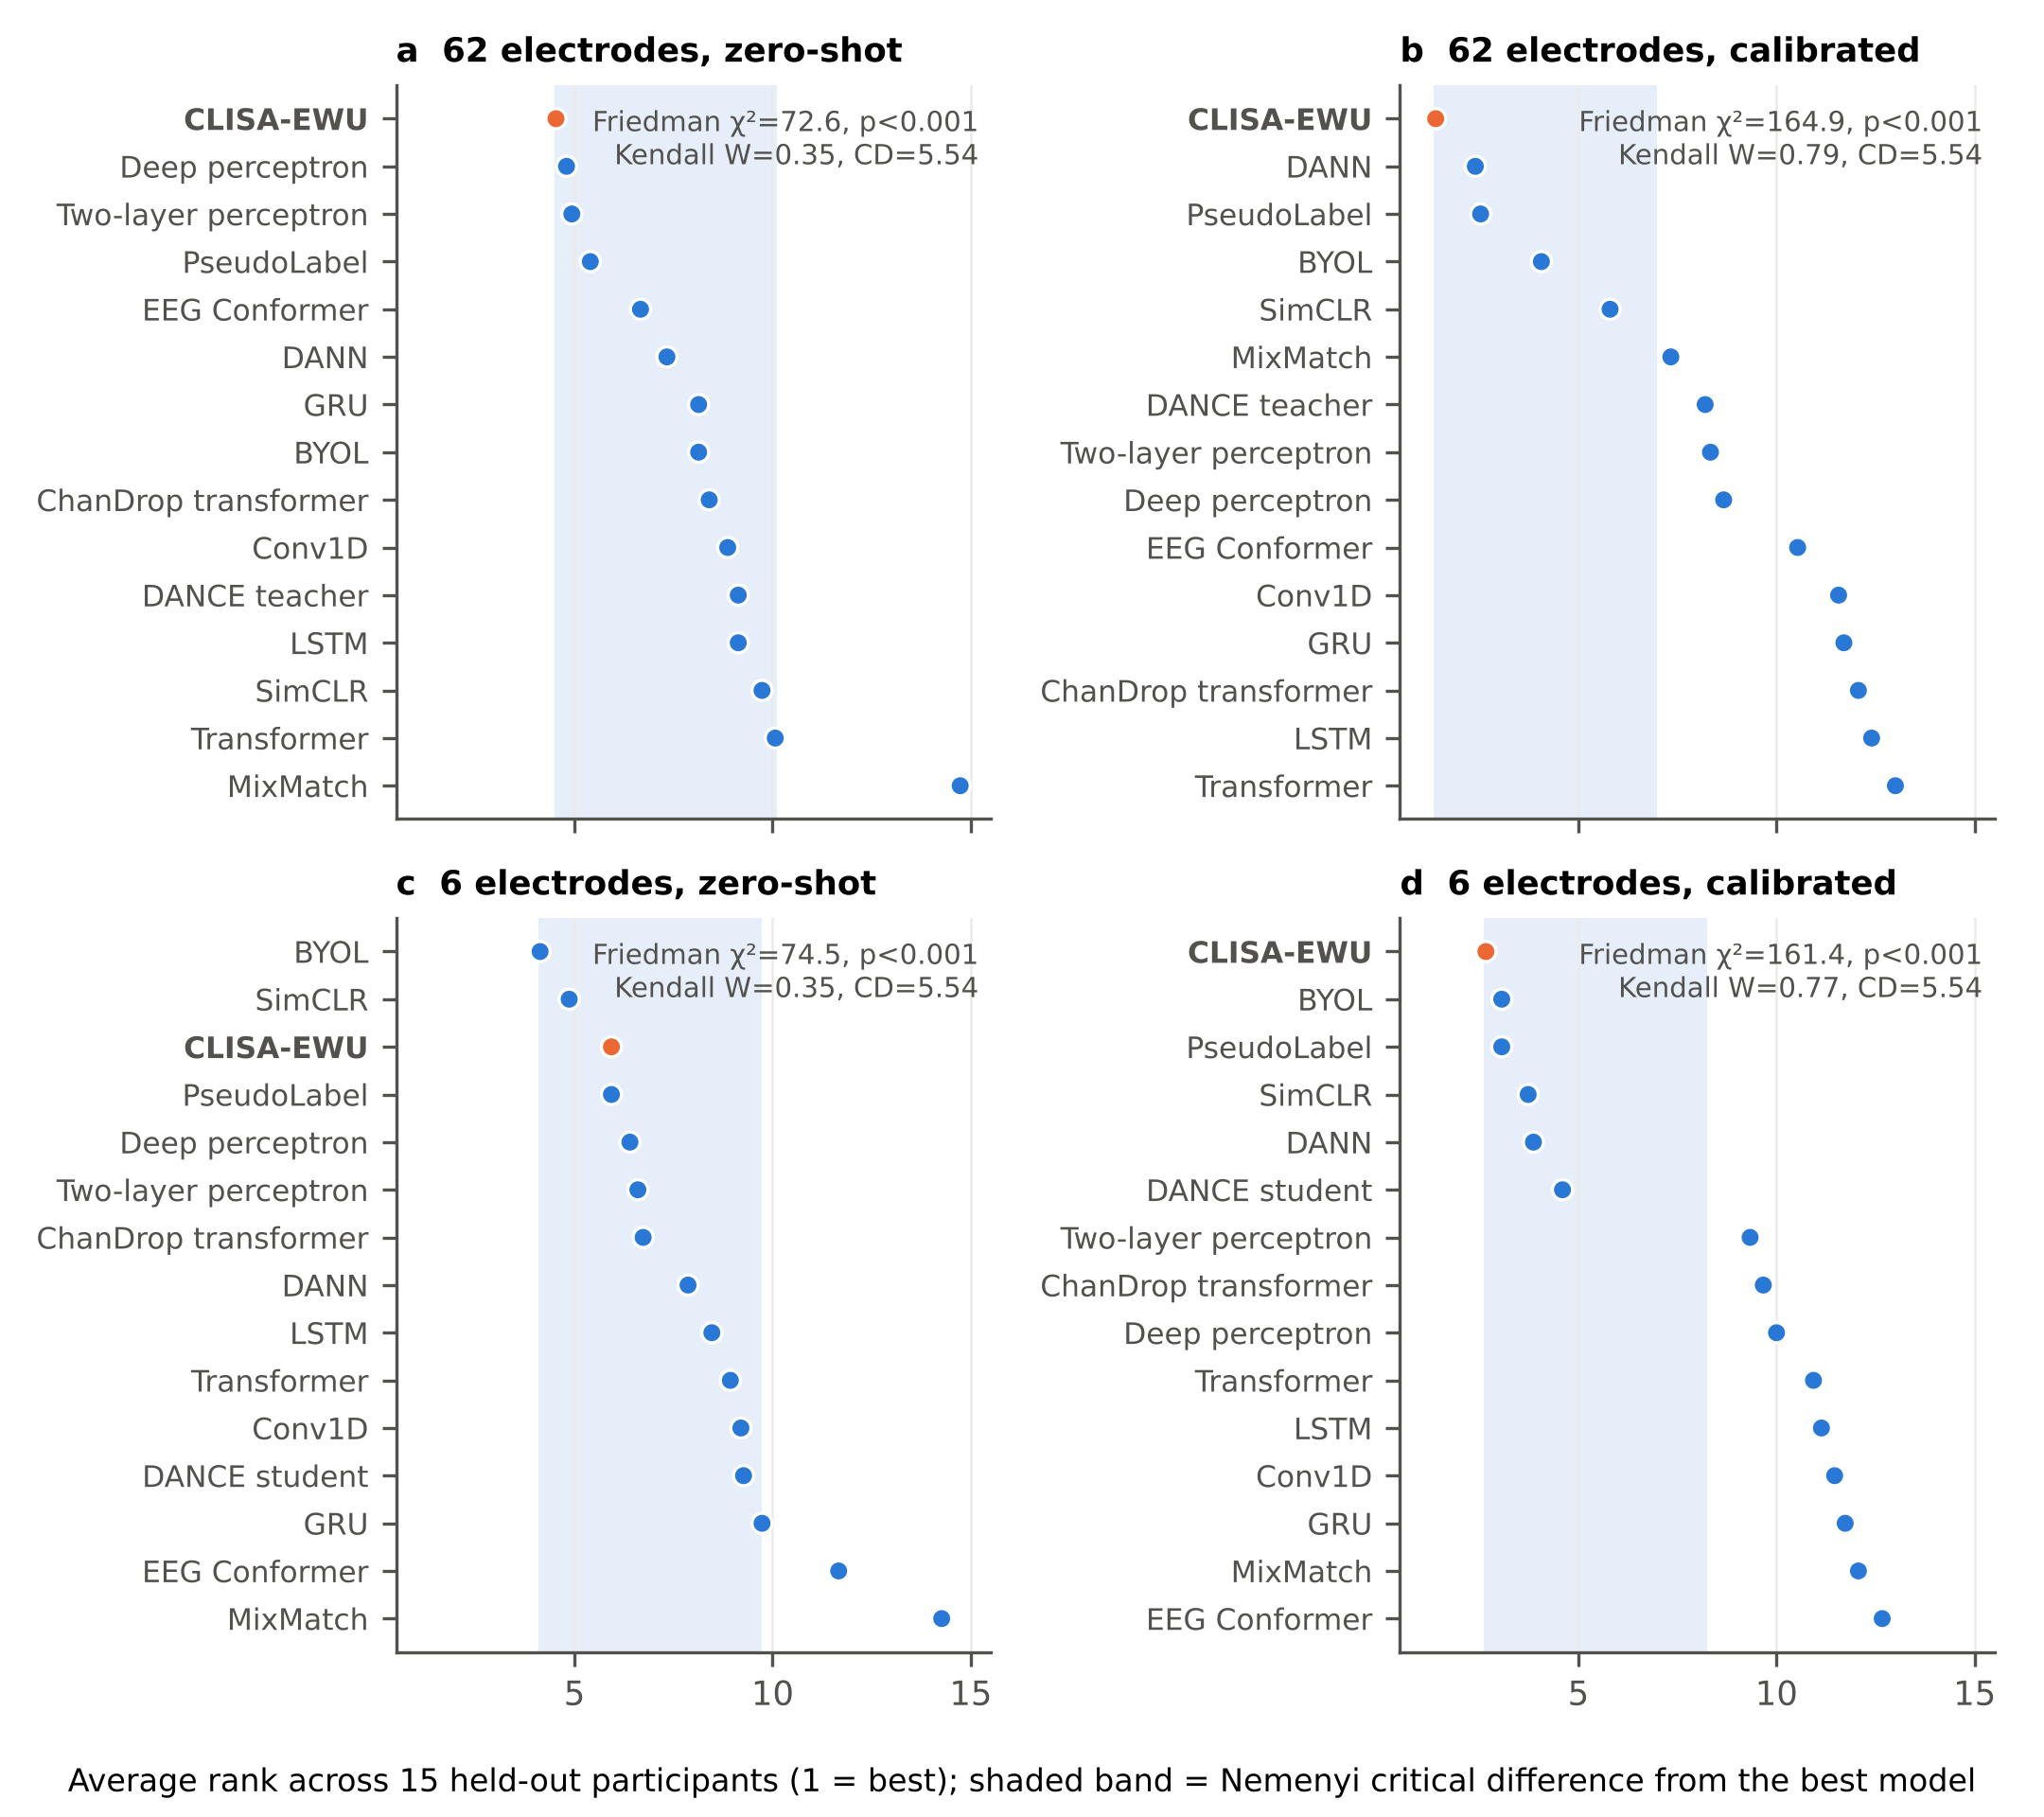
\includegraphics[width=1\linewidth,height=0.62\textheight,keepaspectratio]{figures/new_average_ranks_cd.png}
  \caption{\textbf{Average ranks of the deep models across participants.} Friedman average rank of each model over the 15 held-out participants (1 = best) for (a) 62 electrodes zero-shot, (b) 62 electrodes calibrated, (c) six electrodes zero-shot and (d) six electrodes calibrated. The shaded band extends one Nemenyi critical difference (CD = 5.54) from the best model; models inside it are not significantly different from the best at α = 0.05. CLISA-EWU is shown in orange.}
  \label{fig:cd}
\end{figure}


\subsection{Effect sizes}
Paired effect sizes (Table~\ref{tab:paired}) separate statistical from practical significance. After calibration with 62 electrodes, the advantage of CLISA-EWU over BYOL and SimCLR was very large (\emph{d}\textsubscript{z} = 2.04 and 2.62; \emph{r}\textsubscript{rb} = 1.00, with all 15 participants favouring CLISA-EWU), whereas its advantage over PseudoLabel and DANN was large in standardised terms (\emph{d}\textsubscript{z} = 0.98 and 0.82) but small in absolute terms (2.1 and 1.6 percentage points), and only the PseudoLabel difference survived Holm correction. With six electrodes, effects against the self-supervised and semi-supervised models were small (\emph{d}\textsubscript{z} = 0.14–0.30) and non-significant. Zero-shot, CLISA-EWU differed meaningfully only from EEG Conformer with six electrodes (5.3 points, \emph{d}\textsubscript{z} = 1.38, Holm p = 0.001); its differences from the perceptrons were negligible (\emph{d}\textsubscript{z} = 0.14–0.32).


\subsection{Electrode reduction}
Reducing the montage from 62 to six electrodes lowered calibrated accuracy for CLISA-EWU by 5.8 percentage points (Wilcoxon p < 0.001), a retention of 91.4\% (95\% CI 87.9–95.0\%; Fig.~\ref{fig:subj}b, Fig.~\ref{fig:core}a). Zero-shot retention was lower, at 83.6\%. Retention differed between models (Fig.~\ref{fig:core}b): BYOL and SimCLR performed as well or better with six electrodes than with 62, whereas EEG Conformer retained 78.5\%. After calibration, every six-electrode contrastive, domain-adversarial and pseudo-label model remained above chance for every participant (CLISA-EWU minimum 0.518).

\begin{figure}[!htbp]
  \centering
  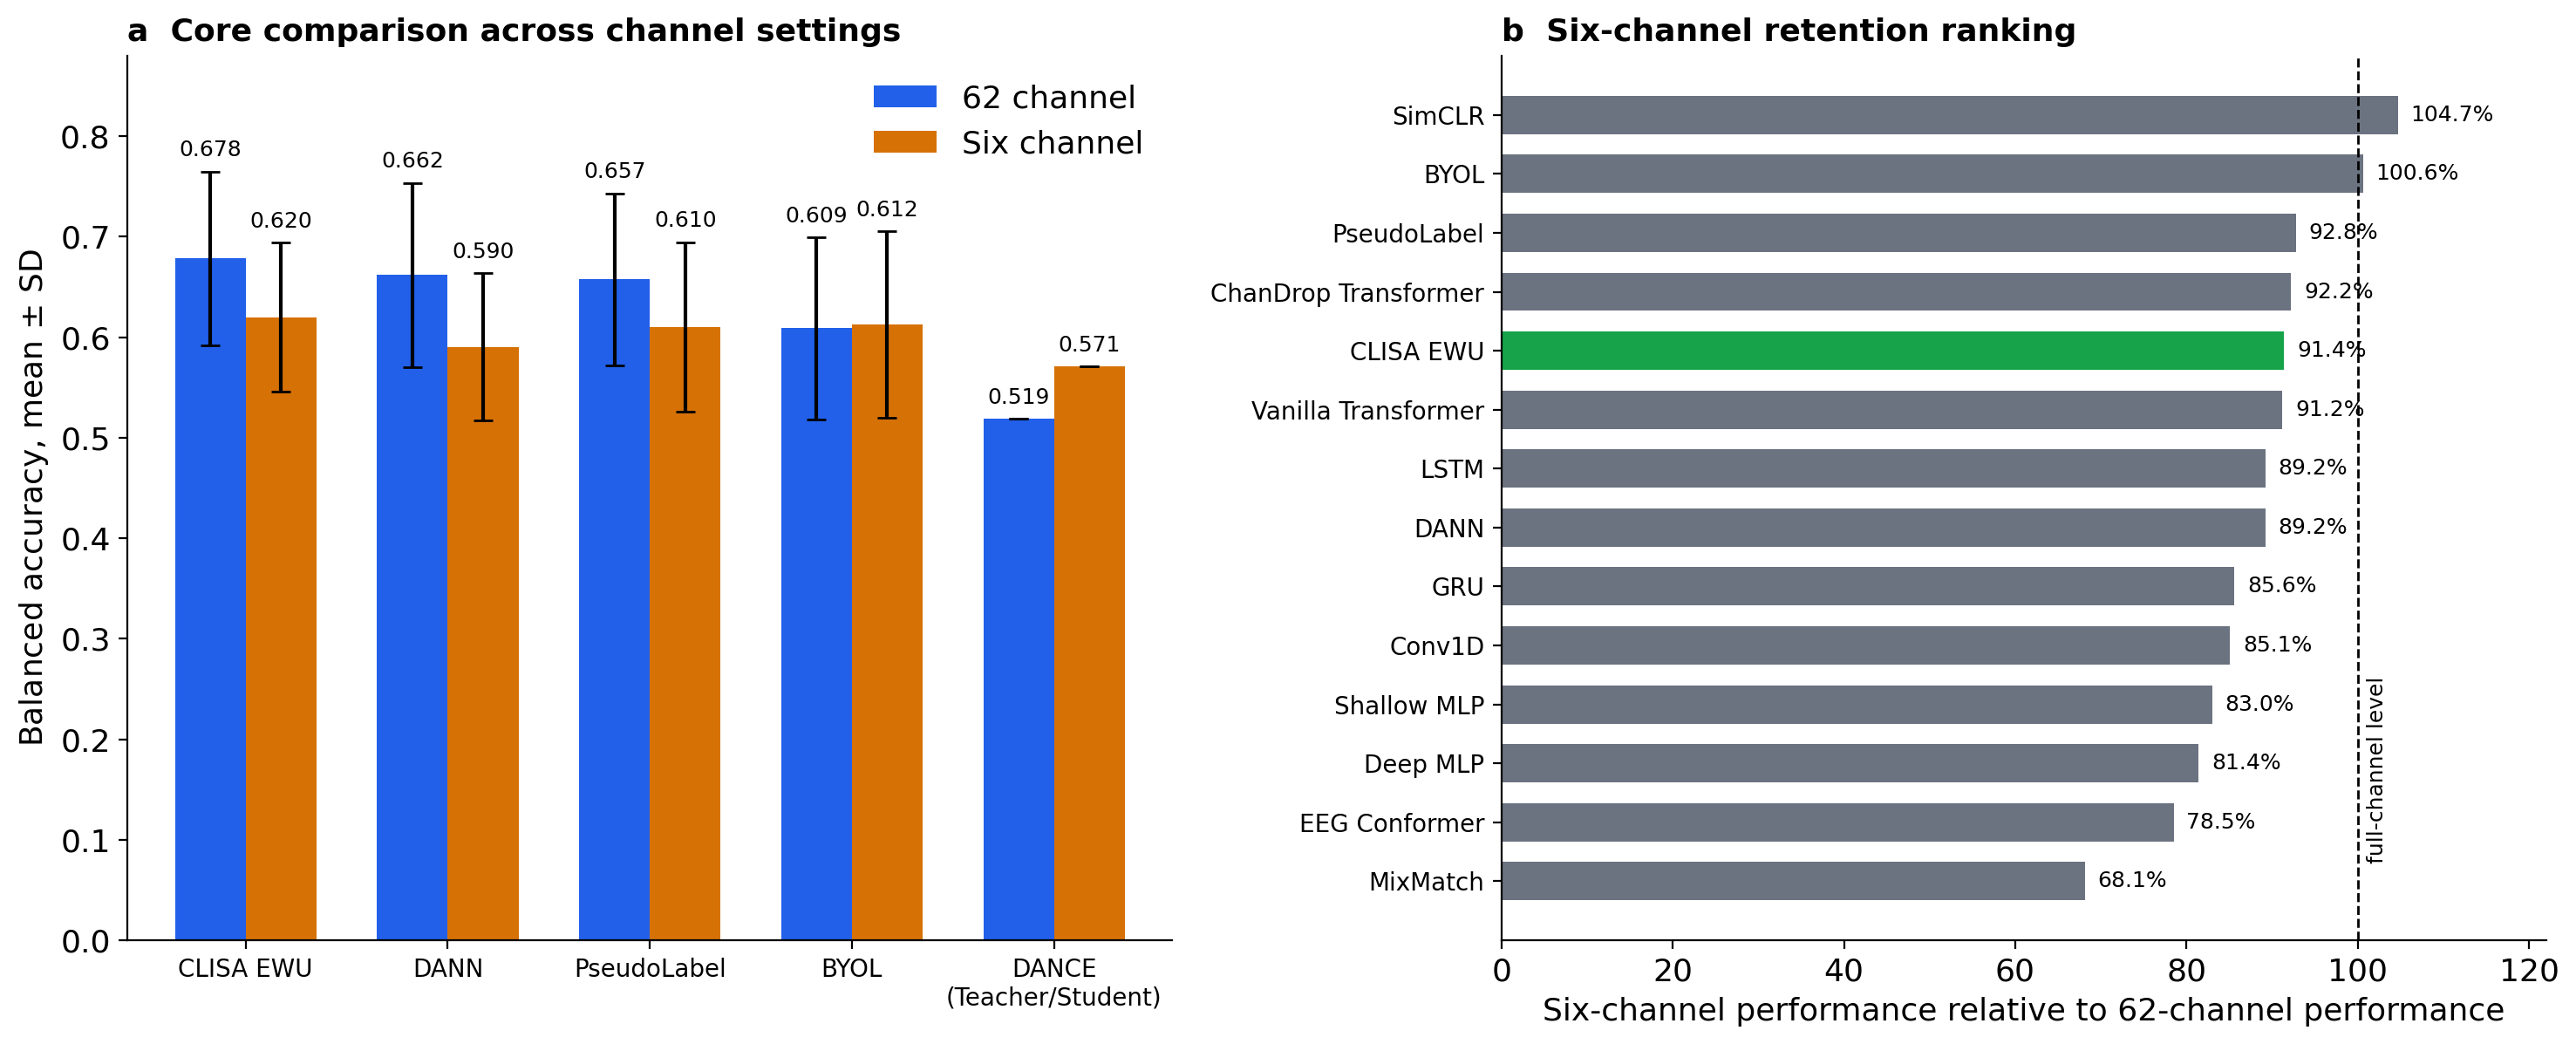
\includegraphics[width=1\linewidth,height=0.62\textheight,keepaspectratio]{figures/thesis_fig06_core_comparison_retention.png}
  \caption{\textbf{Electrode reduction.} (a) Calibrated accuracy (mean ± s.d. over 45 runs) with 62 and six electrodes for CLISA-EWU, DANN, PseudoLabel, BYOL and the DANCE teacher→student pair. (b) Six-electrode retention (six-electrode ÷ 62-electrode performance) for all models; the dashed line marks 100\%. The axis label ‘balanced accuracy’ in this thesis figure denotes accuracy (see Methods).}
  \label{fig:core}
\end{figure}


\subsection{Multi-metric evaluation}
Table~\ref{tab:cmext} reports the complete confusion-matrix metric set for CLISA-EWU and DANN. Calibrated CLISA-EWU with 62 electrodes reached an accuracy of 0.678, balanced accuracy 0.676, macro F1 0.673, Cohen’s κ 0.569 (95\% CI 0.519–0.622) and MCC 0.577; with six electrodes the corresponding values were 0.620, 0.615, 0.611, 0.490 (0.449–0.530) and 0.499. On the Landis–Koch scale\cite{landis}, calibrated agreement beyond chance was moderate (κ 0.41–0.60) for both montages, whereas zero-shot agreement was fair with 62 electrodes (κ = 0.31) and at the border of slight and fair with six (κ = 0.21). MCC tracked κ to within 0.01, macro and weighted F1 differed by at most 0.004, and the geometric mean of recalls (0.659 and 0.594 after calibration) stayed close to balanced accuracy, so the results were not driven by class imbalance or by neglect of any class. Mean specificity was high (0.893 and 0.873), indicating that errors were spread across classes rather than concentrated on one. Expressed as an information transfer rate, calibration raised throughput from 3.35 to 9.13 bits min\textsuperscript{−1} with 62 electrodes and from 1.51 to 6.85 bits min\textsuperscript{−1} with six. CLISA-EWU exceeded DANN on every metric in both montages and protocols, by 1.2–3.8 points of κ.

\begin{table}[!htbp]
  \centering
  {\scriptsize\setlength{\tabcolsep}{2.6pt}
  \begin{tabular}{@{}lcccccccccccc@{}}
  \toprule
\textbf{Model} & \textbf{Ch} & \textbf{Protocol} & \textbf{Acc} & \textbf{BA} & \textbf{P\textsubscript{macro}} & \textbf{F1\textsubscript{m}} & \textbf{F1\textsubscript{w}} & \textbf{κ} & \textbf{MCC} & \textbf{G} & \textbf{Spec} & \textbf{ITR} \\
\midrule
DANN & 62 & Zero-shot & 0.458 & 0.459 & 0.479 & 0.455 & 0.456 & 0.278 & 0.282 & 0.436 & 0.820 & 2.76 \\
DANN & 62 & Calibrated & 0.662 & 0.658 & 0.688 & 0.654 & 0.658 & 0.547 & 0.556 & 0.637 & 0.887 & 8.52 \\
DANN & 6 & Zero-shot & 0.396 & 0.397 & 0.404 & 0.386 & 0.387 & 0.195 & 0.199 & 0.359 & 0.799 & 1.50 \\
DANN & 6 & Calibrated & 0.590 & 0.586 & 0.604 & 0.579 & 0.584 & 0.452 & 0.458 & 0.562 & 0.863 & 5.85 \\
CLISA-EWU & 62 & Zero-shot & 0.485 & 0.485 & 0.504 & 0.479 & 0.481 & 0.312 & 0.317 & 0.460 & 0.828 & 3.35 \\
CLISA-EWU & 62 & Calibrated & 0.678 & 0.676 & 0.700 & 0.673 & 0.675 & 0.569 & 0.577 & 0.659 & 0.893 & 9.13 \\
CLISA-EWU & 6 & Zero-shot & 0.405 & 0.407 & 0.412 & 0.398 & 0.398 & 0.207 & 0.212 & 0.374 & 0.802 & 1.51 \\
CLISA-EWU & 6 & Calibrated & 0.620 & 0.615 & 0.641 & 0.611 & 0.615 & 0.490 & 0.499 & 0.594 & 0.873 & 6.84 \\
  \bottomrule
  \end{tabular}}
  \caption{Complete confusion-matrix metrics for CLISA-EWU and DANN (means over 15 participants). Ch = electrodes; BA = balanced accuracy; P\textsubscript{macro} = macro precision; F1\textsubscript{m} and F1\textsubscript{w} = macro and weighted F1; κ = Cohen’s kappa; MCC = Matthews correlation coefficient; G = geometric mean of recalls; Spec = macro specificity; ITR in bits min\textsuperscript{−1} (4-s windows).}
  \label{tab:cmext}
\end{table}


\subsection{Variability across participants and seeds}
Between-participant variability exceeded between-seed variability. With 62 electrodes, calibrated CLISA-EWU ranged from 0.541 (participant 5) to 0.813 (participant 2) across participants, whereas seed means ranged from 0.658 to 0.691 (Fig.~\ref{fig:violin}). The best single runs reached 0.854 with 62 electrodes (participant 15, seed 7) and 0.786 with six (participant 7, seed 1); they are shown for completeness and are not estimates of expected performance. Fine-tuning converged smoothly (Fig.~\ref{fig:loss}).

\begin{figure}[!htbp]
  \centering
  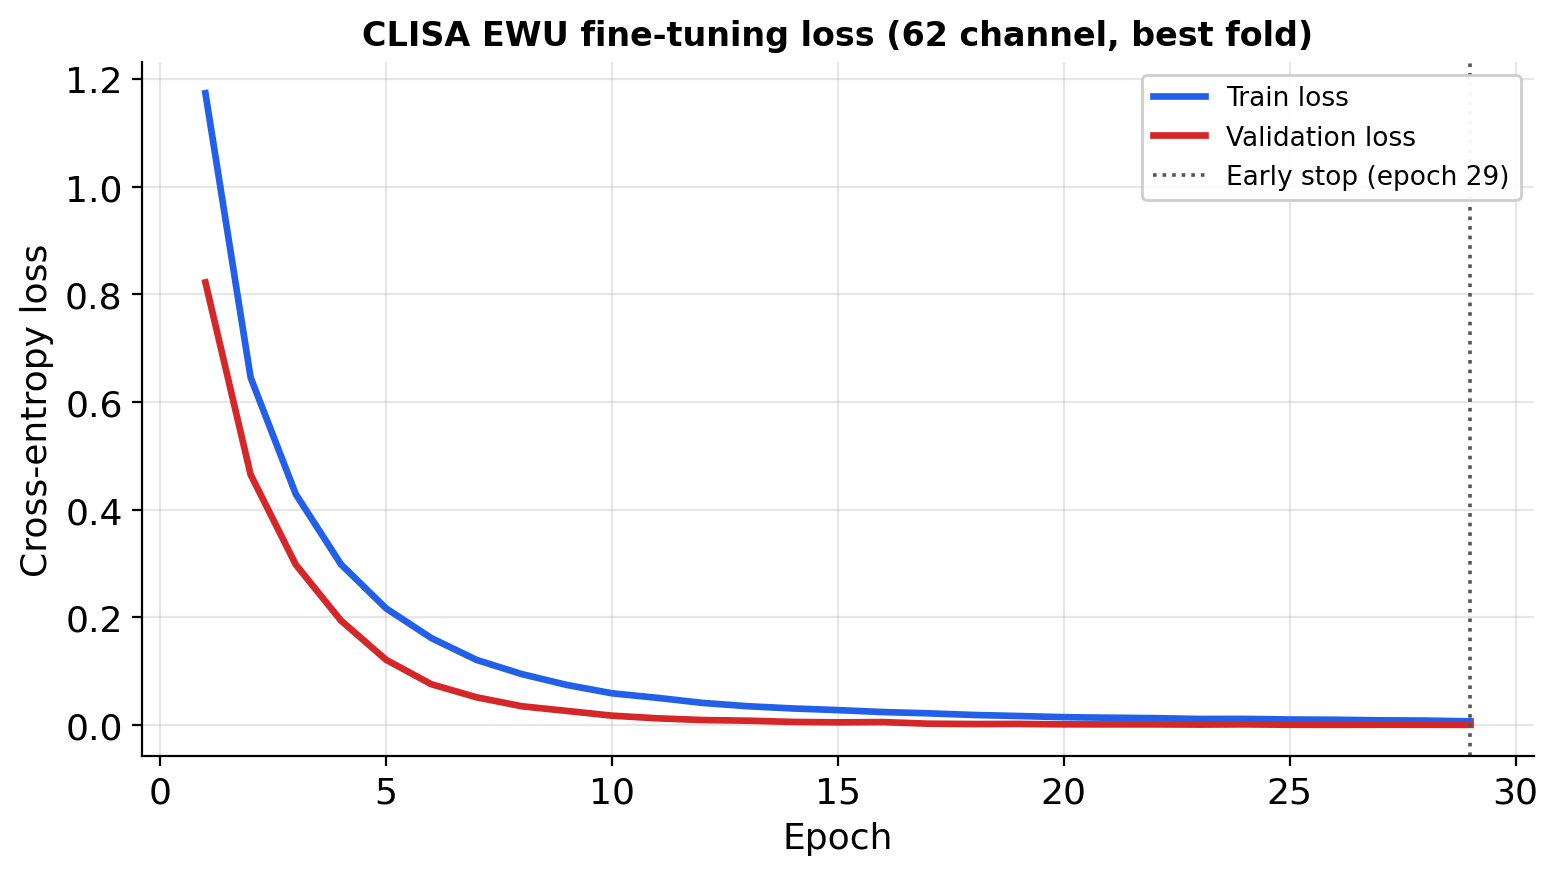
\includegraphics[width=1\linewidth,height=0.62\textheight,keepaspectratio]{figures/thesis_fig10_finetune_loss.png}
  \caption{\textbf{Fine-tuning convergence.} Training and validation cross-entropy for CLISA-EWU with 62 electrodes in the best run (participant 15, seed 7); early stopping at epoch 29. Validation loss lies below training loss because dropout is active during training and validation windows share participants and trials with training windows.}
  \label{fig:loss}
\end{figure}

A two-way decomposition (Table~\ref{tab:vardec}) quantified the sources of this variability. Zero-shot with 62 electrodes, participant identity explained 96.9\% of the variance in CLISA-EWU accuracy and the seed only 0.05\% (ICC(3,1) = 0.95). After calibration, the participant share fell to 77.8\%, residual variance rose to 19.3\% and the ICC dropped to 0.70; with six electrodes the seed effect became significant (F = 4.49, p = 0.020; ICC = 0.53). Because the seed also determines which 20 windows are drawn for calibration, this increase reflects sensitivity to the choice of calibration samples, which argues for averaging over several calibration draws in practice.

\begin{table}[!htbp]
  \centering
  {\footnotesize\setlength{\tabcolsep}{3.5pt}
  \begin{tabular}{@{}lccccccc@{}}
  \toprule
\textbf{Ch} & \textbf{Protocol} & \textbf{Participant (\%)} & \textbf{Seed (\%)} & \textbf{Residual (\%)} & \textbf{F participant (p)} & \textbf{F seed (p)} & \textbf{ICC(3,1)} \\
\midrule
62 & Zero-shot & 96.9 & 0.0 & 3.1 & 63.50 (<0.001) & 0.22 (0.805) & 0.95 \\
62 & Calibrated & 77.8 & 2.9 & 19.3 & 8.06 (<0.001) & 2.13 (0.138) & 0.70 \\
6 & Zero-shot & 84.3 & 2.3 & 13.4 & 12.54 (<0.001) & 2.40 (0.109) & 0.79 \\
6 & Calibrated & 62.3 & 9.2 & 28.6 & 4.36 (<0.001) & 4.49 (0.020) & 0.53 \\
  \bottomrule
  \end{tabular}}
  \caption{Decomposition of CLISA-EWU accuracy variance into participant, seed and residual components (two-way ANOVA without replication) and consistency across seeds (ICC(3,1)).}
  \label{tab:vardec}
\end{table}


\subsection{Who benefits from calibration}
Calibration gain was negatively correlated with zero-shot accuracy (Spearman ρ = −0.60, p = 0.017 with 62 electrodes; ρ = −0.58, p = 0.024 with six; Fig.~\ref{fig:gain}a): participants who were decoded worst without calibration gained most, up to 39 percentage points for participant 11. Part of this association is expected from regression to the mean, because the gain contains the zero-shot score. Across montages, participants’ calibrated accuracies were strongly correlated (ρ = 0.80, p < 0.001) whereas their zero-shot accuracies were not (ρ = −0.05, p = 0.86; Fig.~\ref{fig:gain}b), so after calibration a participant who is decoded well with 62 electrodes is also decoded well with six. Across models, participant rankings before and after calibration were almost identical for supervised networks (ρ = 0.94–1.00) but less so for the adaptable models (ρ = 0.43–0.93), consistent with calibration substantively changing only the latter.

\begin{figure}[!htbp]
  \centering
  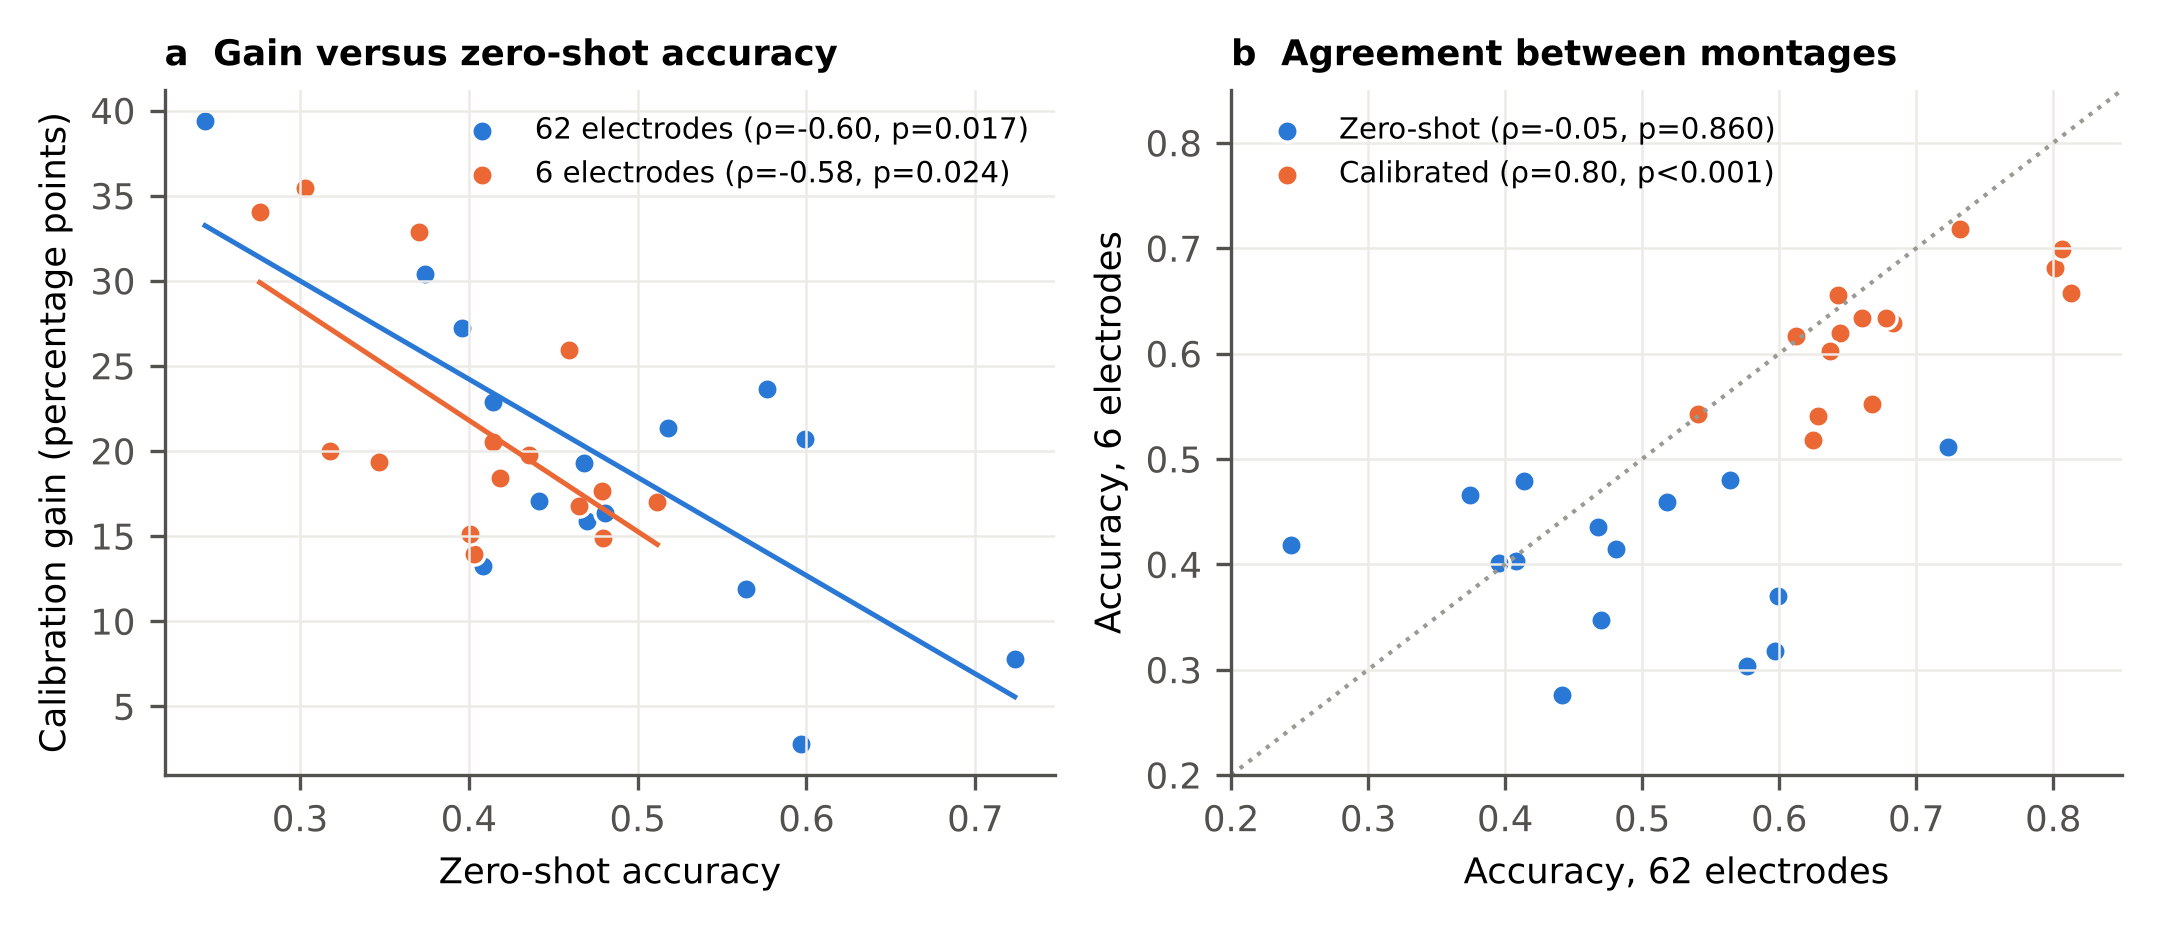
\includegraphics[width=1\linewidth,height=0.62\textheight,keepaspectratio]{figures/new_gain_and_agreement.png}
  \caption{\textbf{Who benefits from calibration.} (a) Calibration gain versus zero-shot accuracy for each participant with 62 and six electrodes, with least-squares lines and Spearman correlations. (b) Agreement of participant accuracy between montages, zero-shot and calibrated; the dotted line marks equality.}
  \label{fig:gain}
\end{figure}


\subsection{Class-level behaviour and electrode importance}
Per-class metrics (Table~\ref{tab:perclass}, Fig.~\ref{fig:perclass}) and the mean confusion matrices over all 45 runs (Fig.~\ref{fig:meancm}) show where the errors arose. After calibration with 62 electrodes, sad had the highest recall (0.733) but the lowest specificity (0.858), because it attracted errors from fear (16.9\% of fear windows) and happy (14.3\%); neutral had the highest precision (0.790) and F1 (0.728). Fear was the hardest class in both montages (F1 = 0.621 and 0.565) and was confused mostly with sad. Electrode reduction affected classes unequally: recall fell by 9.6 percentage points for happy, 7.4 for fear, 4.4 for sad and 2.9 for neutral. Zero-shot, the confusion matrices were diffuse and biased towards fear, which received 21.0\% of neutral, 24.5\% of sad and 21.3\% of happy windows with 62 electrodes; calibration removed most of this bias. In the best single runs (Fig.~\ref{fig:conf}), sad recall reached 100\% with 62 electrodes.

\begin{table}[!htbp]
  \centering
  {\footnotesize\setlength{\tabcolsep}{3.5pt}
  \begin{tabular}{@{}lcccccccc@{}}
  \toprule
\textbf{Class} & \textbf{P (ZS)} & \textbf{R (ZS)} & \textbf{F1 (ZS)} & \textbf{Spec (ZS)} & \textbf{P (Cal)} & \textbf{R (Cal)} & \textbf{F1 (Cal)} & \textbf{Spec (Cal)} \\
\midrule
\multicolumn{9}{@{}l}{\textit{62 electrodes}} \\
Neutral & 0.595 & 0.535 & 0.541 & 0.848 & 0.790 & 0.697 & 0.728 & 0.919 \\
Sad & 0.539 & 0.464 & 0.480 & 0.837 & 0.687 & 0.733 & 0.695 & 0.858 \\
Fear & 0.393 & 0.438 & 0.408 & 0.776 & 0.675 & 0.604 & 0.621 & 0.895 \\
Happy & 0.490 & 0.504 & 0.488 & 0.852 & 0.648 & 0.671 & 0.647 & 0.898 \\
\midrule
\multicolumn{9}{@{}l}{\textit{Six electrodes}} \\
Neutral & 0.489 & 0.430 & 0.446 & 0.829 & 0.674 & 0.668 & 0.659 & 0.870 \\
Sad & 0.419 & 0.399 & 0.402 & 0.787 & 0.636 & 0.689 & 0.644 & 0.828 \\
Fear & 0.336 & 0.327 & 0.322 & 0.797 & 0.645 & 0.530 & 0.565 & 0.901 \\
Happy & 0.402 & 0.473 & 0.422 & 0.795 & 0.607 & 0.575 & 0.577 & 0.892 \\
  \bottomrule
  \end{tabular}}
  \caption{Per-class precision (P), recall (R), F1 and specificity (Spec) of CLISA-EWU, zero-shot (ZS) and calibrated (Cal), means over 15 participants.}
  \label{tab:perclass}
\end{table}

\begin{figure}[!htbp]
  \centering
  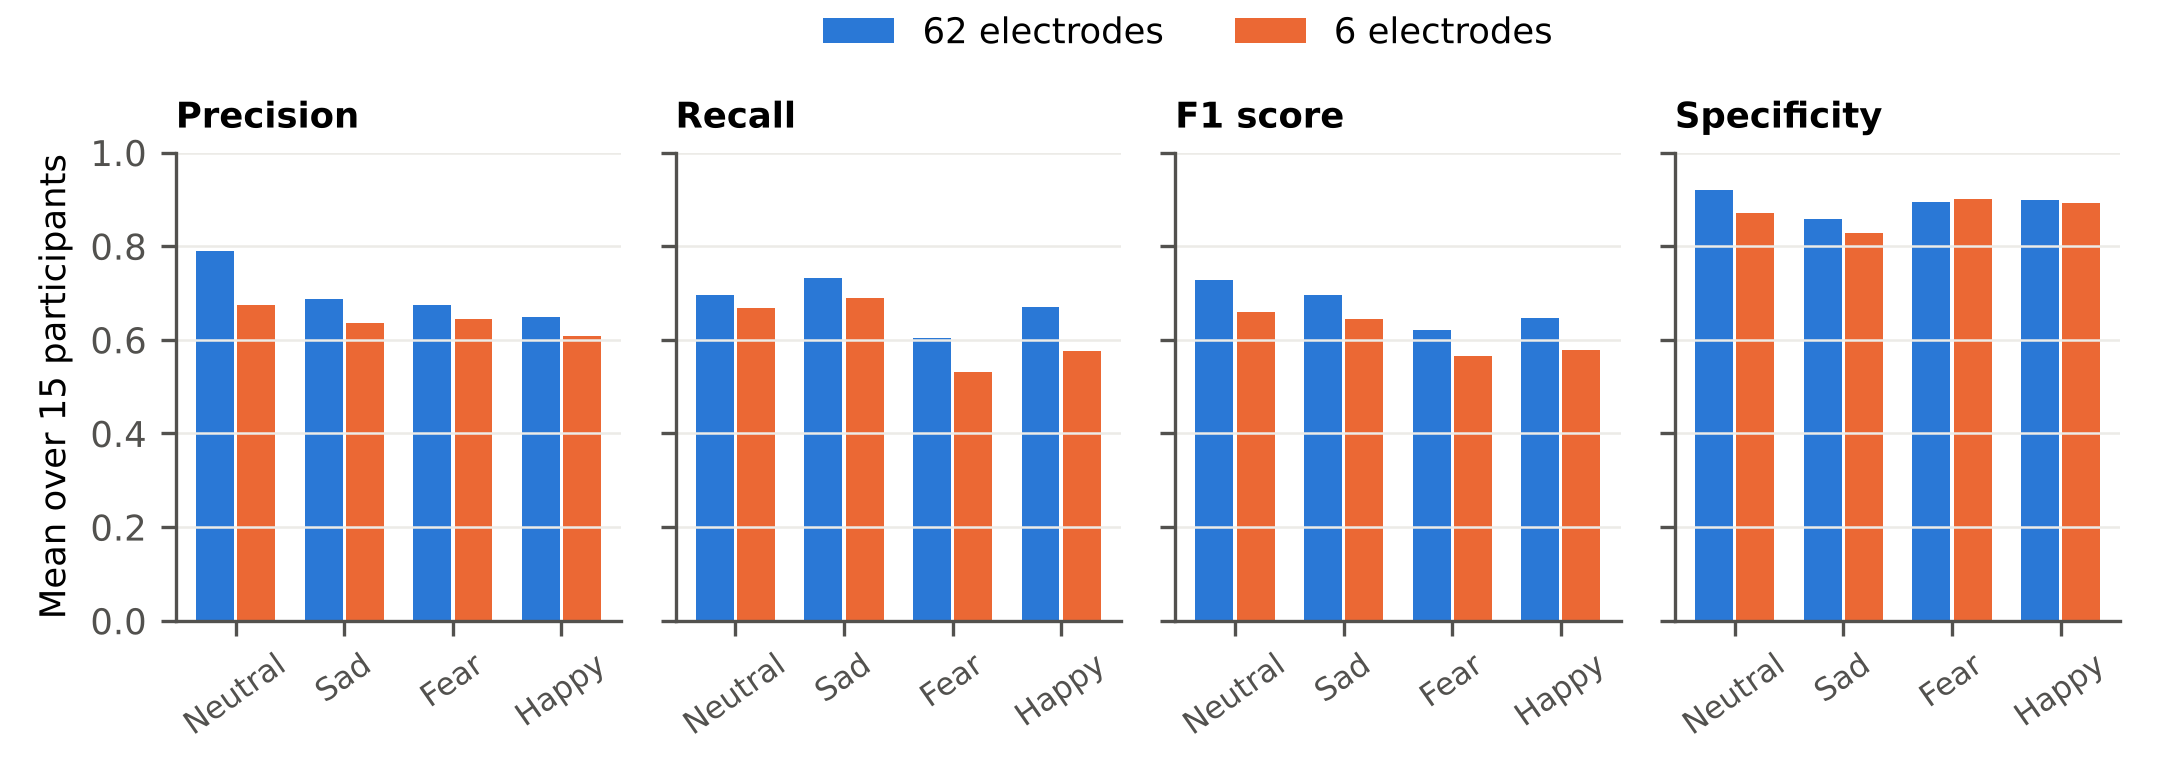
\includegraphics[width=1\linewidth,height=0.62\textheight,keepaspectratio]{figures/new_per_class_metrics.png}
  \caption{\textbf{Per-class metrics of calibrated CLISA-EWU.} Precision, recall, F1 score and specificity for each emotion with 62 and six electrodes, means over 15 held-out participants.}
  \label{fig:perclass}
\end{figure}

\begin{figure}[!htbp]
  \centering
  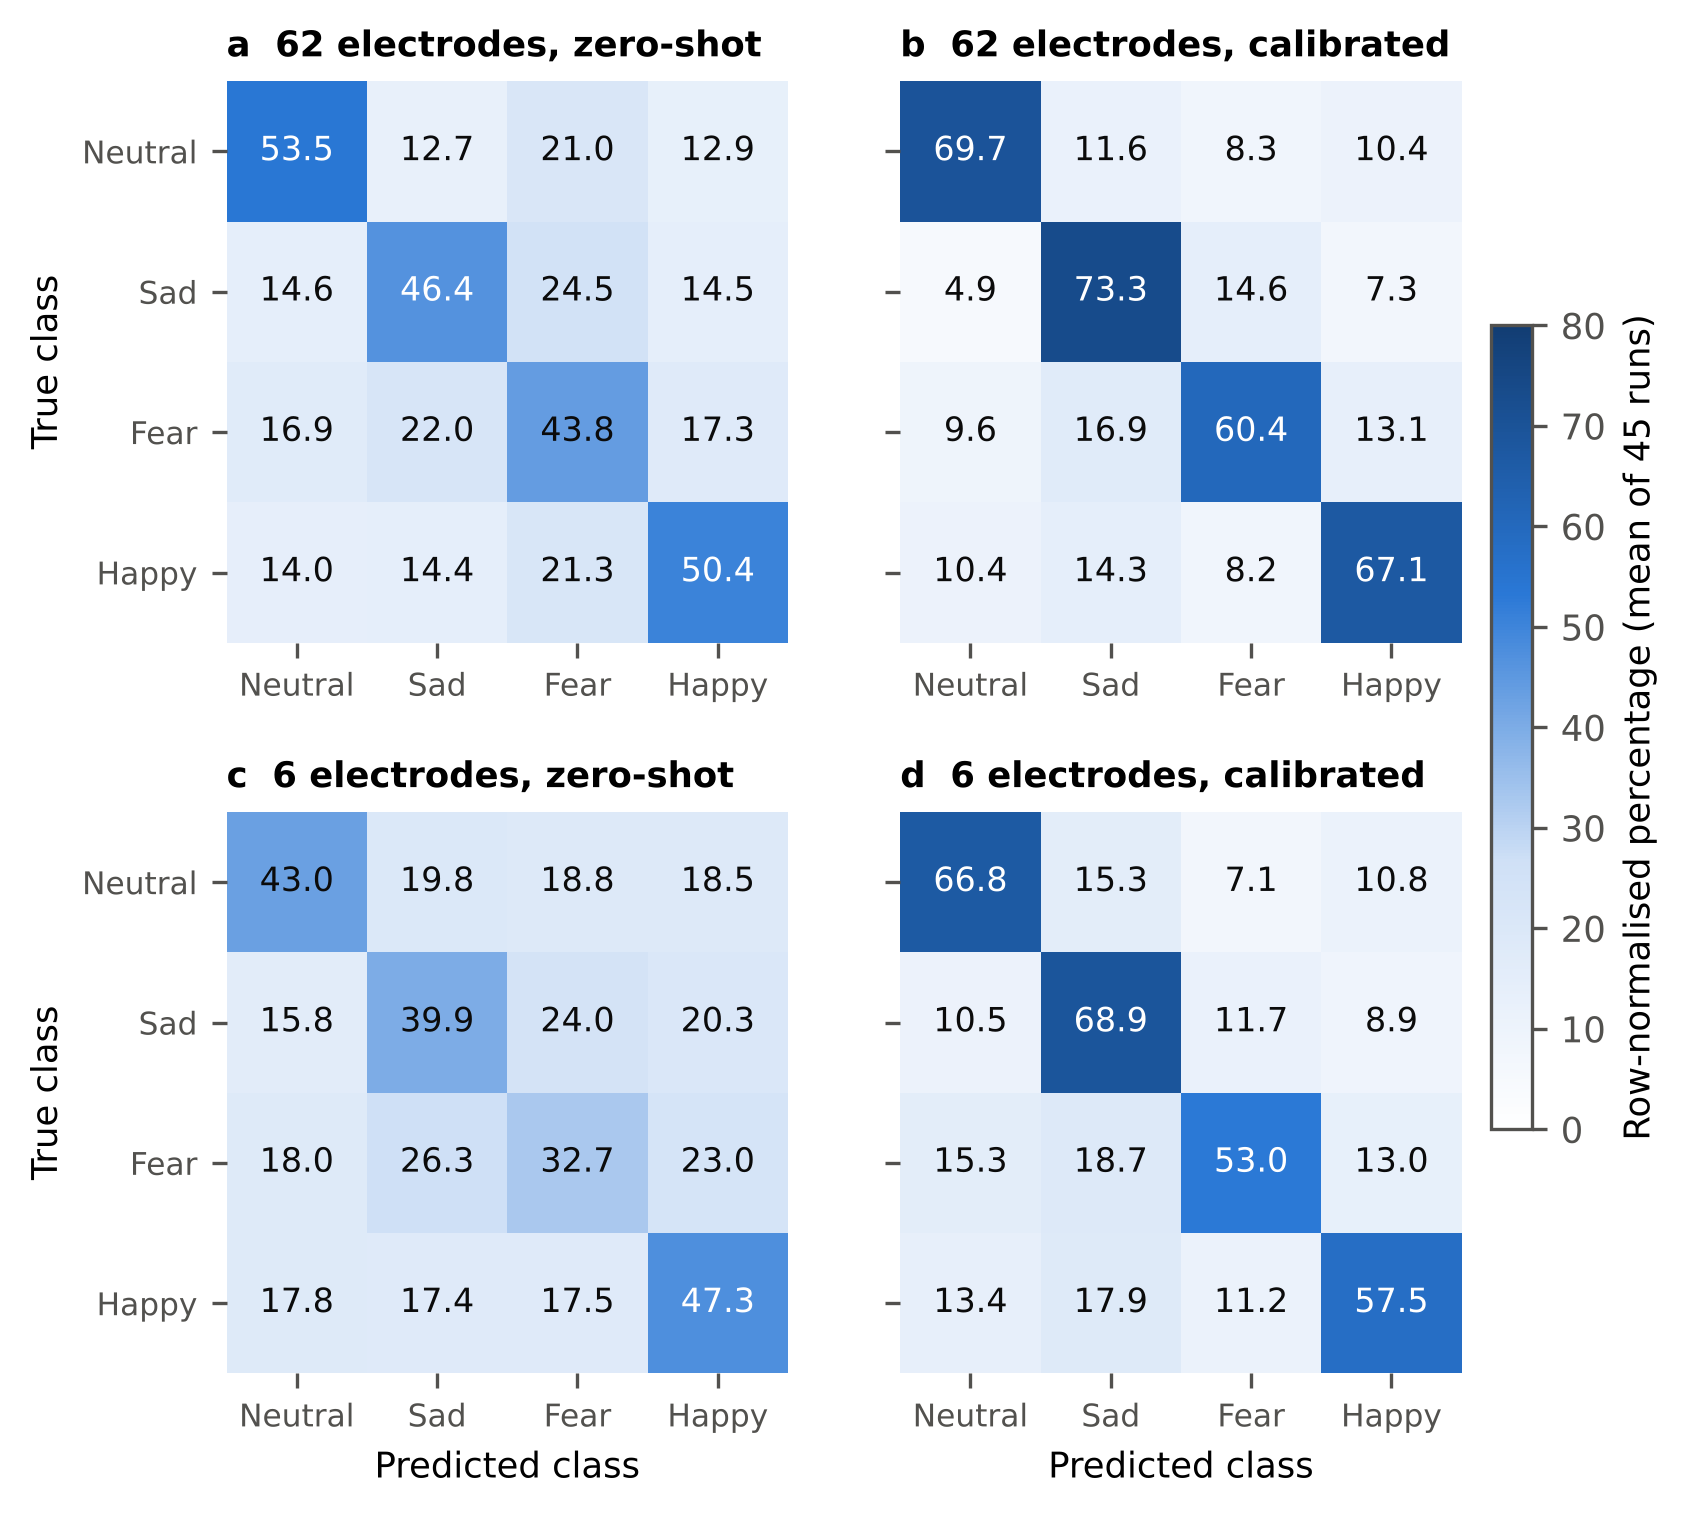
\includegraphics[width=1\linewidth,height=0.62\textheight,keepaspectratio]{figures/new_mean_confusion.png}
  \caption{\textbf{Mean confusion matrices of CLISA-EWU.} Row-normalised percentages averaged over all 45 runs for (a) 62 electrodes zero-shot, (b) 62 electrodes calibrated, (c) six electrodes zero-shot and (d) six electrodes calibrated. Diagonal cells are per-class recall.}
  \label{fig:meancm}
\end{figure}

\begin{figure}[!htbp]
  \centering
  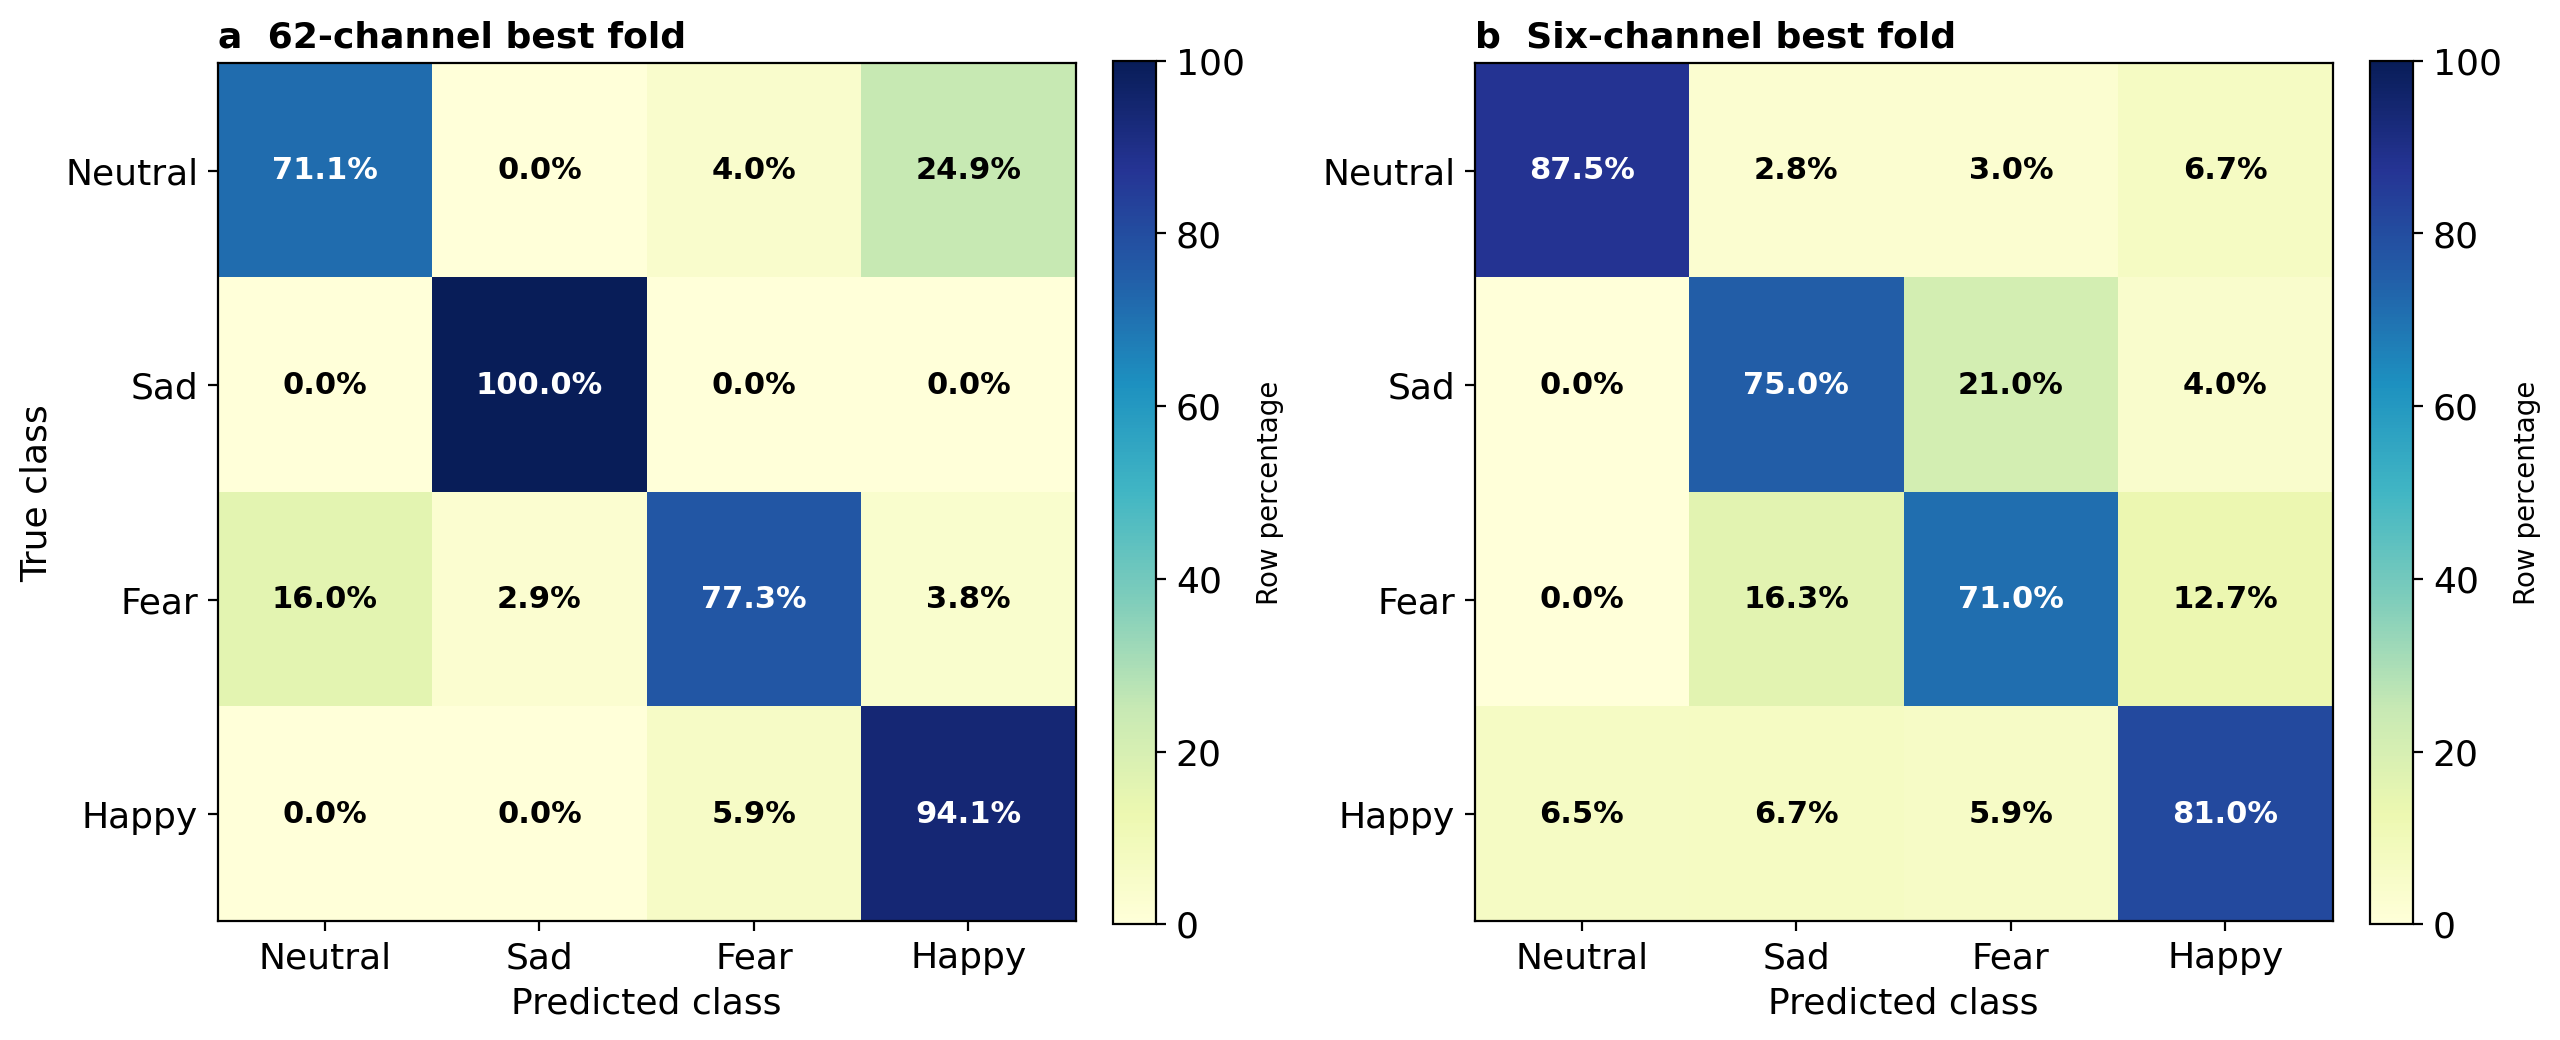
\includegraphics[width=1\linewidth,height=0.62\textheight,keepaspectratio]{figures/thesis_fig08_best_run_confusion.png}
  \caption{\textbf{Confusion matrices of CLISA-EWU in the best single runs.} Row-normalised percentages after calibration with (a) 62 electrodes (participant 15, seed 7) and (b) six electrodes (participant 7, seed 1). Best runs illustrate class-level behaviour and are not representative; mean per-class recall over all runs is reported in the text.}
  \label{fig:conf}
\end{figure}

Electrode importance differed by class (Fig.~\ref{fig:shap}). For happy, the wearable electrodes FP1 and FP2 ranked second and sixth of 62. For sad, FP1 and F8 ranked fourth and seventh, and the most important electrode was the adjacent midline FPZ. For neutral, FP2 ranked third. For fear, the most important electrodes were parieto-occipital (POZ, PO8), and only F7 among the wearable electrodes ranked in the top five, consistent with fear being the class most affected by electrode reduction. This analysis is based on a single run and is exploratory.

\begin{figure}[!htbp]
  \centering
  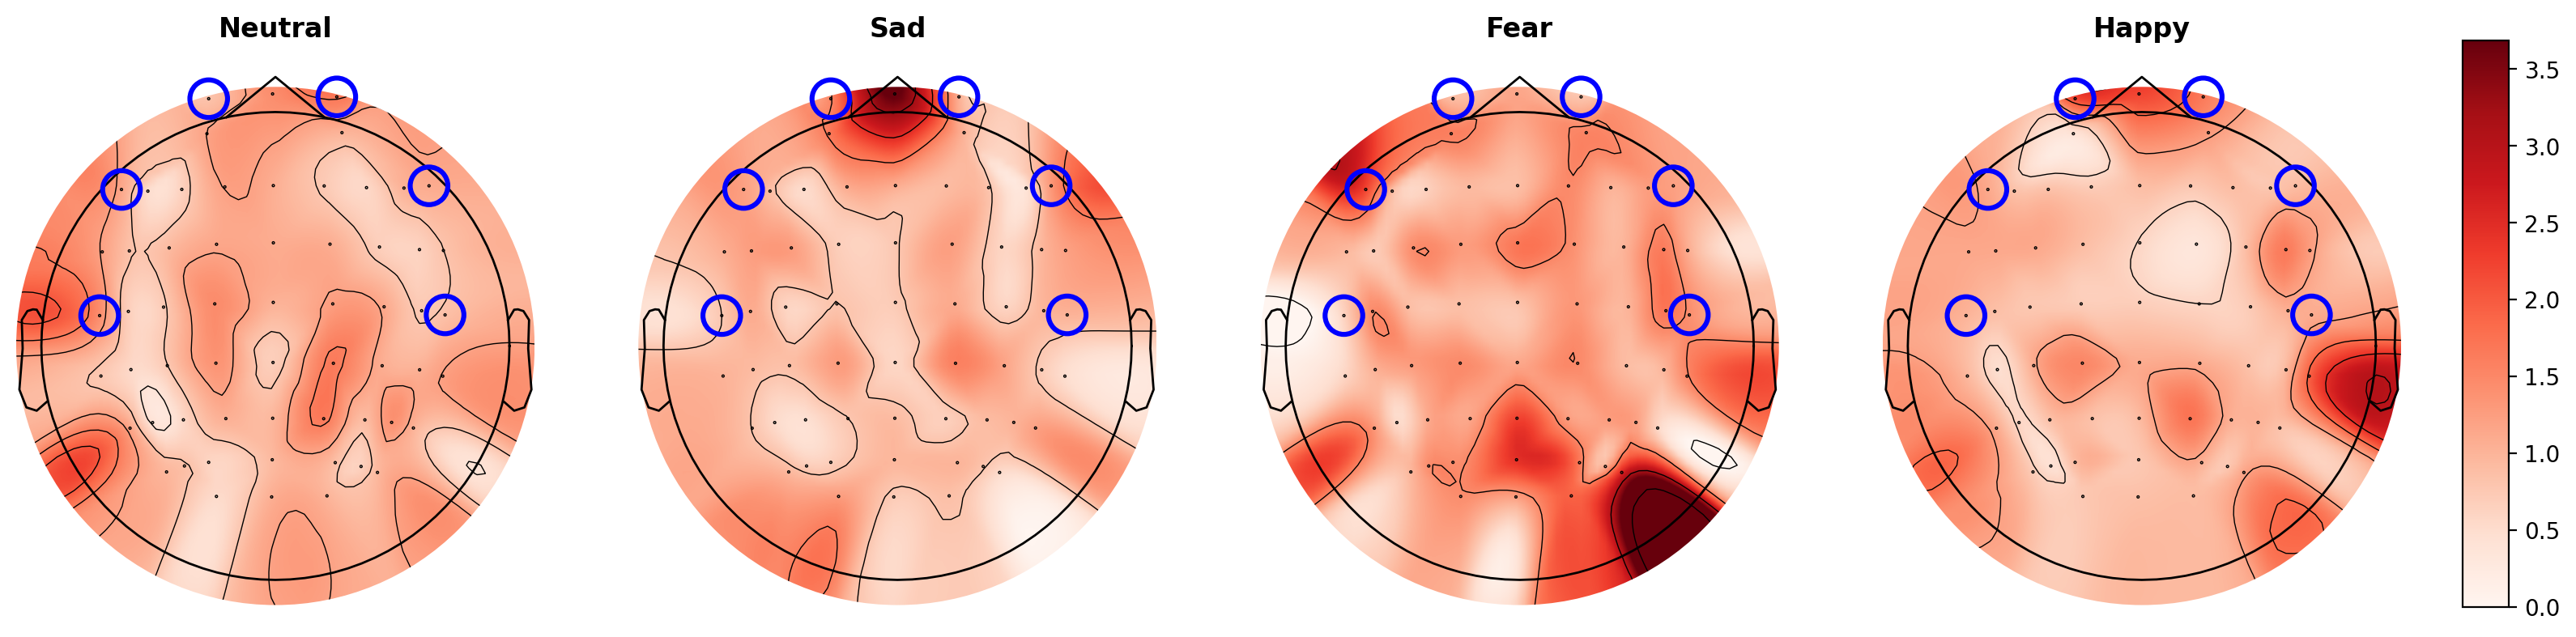
\includegraphics[width=1\linewidth,height=0.62\textheight,keepaspectratio]{figures/thesis_fig14_shap_topomaps.png}
  \caption{\textbf{Electrode importance by predicted class.} SHAP attributions summed over five frequency bands per electrode for neutral, sad, fear and happy (left to right), CLISA-EWU with 62 electrodes, best run; shared colour scale. Blue circles mark the six-electrode wearable subset. Single-run, exploratory analysis.}
  \label{fig:shap}
\end{figure}


\subsection{Representation geometry}
In the raw feature space, emotion classes were not separable (emotion silhouette −0.017 with 62 electrodes and −0.013 with six; Table~\ref{tab:cluster}). In the CLISA-EWU embedding, emotion silhouette rose to 0.220 (62 electrodes) and 0.046 (six), Davies–Bouldin indices fell, and participant silhouettes were negative (−0.098 and −0.057), indicating that participant identity did not dominate the embedding (Fig.~\ref{fig:tsne}). These embeddings were computed on all 15 participants with the best-run model, 14 of whom contributed labelled training data, so the emotion structure partly reflects supervised fitting \pending{recompute on held-out participants only}.

\begin{table}[!htbp]
  \centering
  {\small\setlength{\tabcolsep}{5pt}
  \begin{tabular}{@{}lcccc@{}}
  \toprule
\textbf{Feature space} & \textbf{Labels (clusters)} & \textbf{Silhouette} & \textbf{Davies–Bouldin} & \textbf{Calinski–Harabasz} \\
\midrule
Raw, 62 electrodes & Emotion (4) & −0.017 & 7.68 & 511.8 \\
Raw, 62 electrodes & Participant (15) & −0.034 & 1.40 × 10\textsuperscript{5} & <0.1 \\
CLISA-EWU, 62 electrodes & Emotion (4) & 0.220 & 1.64 & 7309.0 \\
CLISA-EWU, 62 electrodes & Participant (15) & −0.098 & 11.10 & 84.4 \\
Raw, six electrodes & Emotion (4) & −0.013 & 8.16 & 536.3 \\
Raw, six electrodes & Participant (15) & −0.045 & 5.56 × 10\textsuperscript{4} & <0.1 \\
CLISA-EWU, six electrodes & Emotion (4) & 0.046 & 3.75 & 1434.1 \\
CLISA-EWU, six electrodes & Participant (15) & −0.057 & 10.09 & 159.6 \\
  \bottomrule
  \end{tabular}}
  \caption{Clustering metrics for raw features and CLISA-EWU embeddings. Higher silhouette and Calinski–Harabasz and lower Davies–Bouldin values indicate tighter clusters. Embeddings were computed with the best-run model on all 15 participants (14 of whom were in its training set).}
  \label{tab:cluster}
\end{table}

\begin{figure}[!htbp]
  \centering
  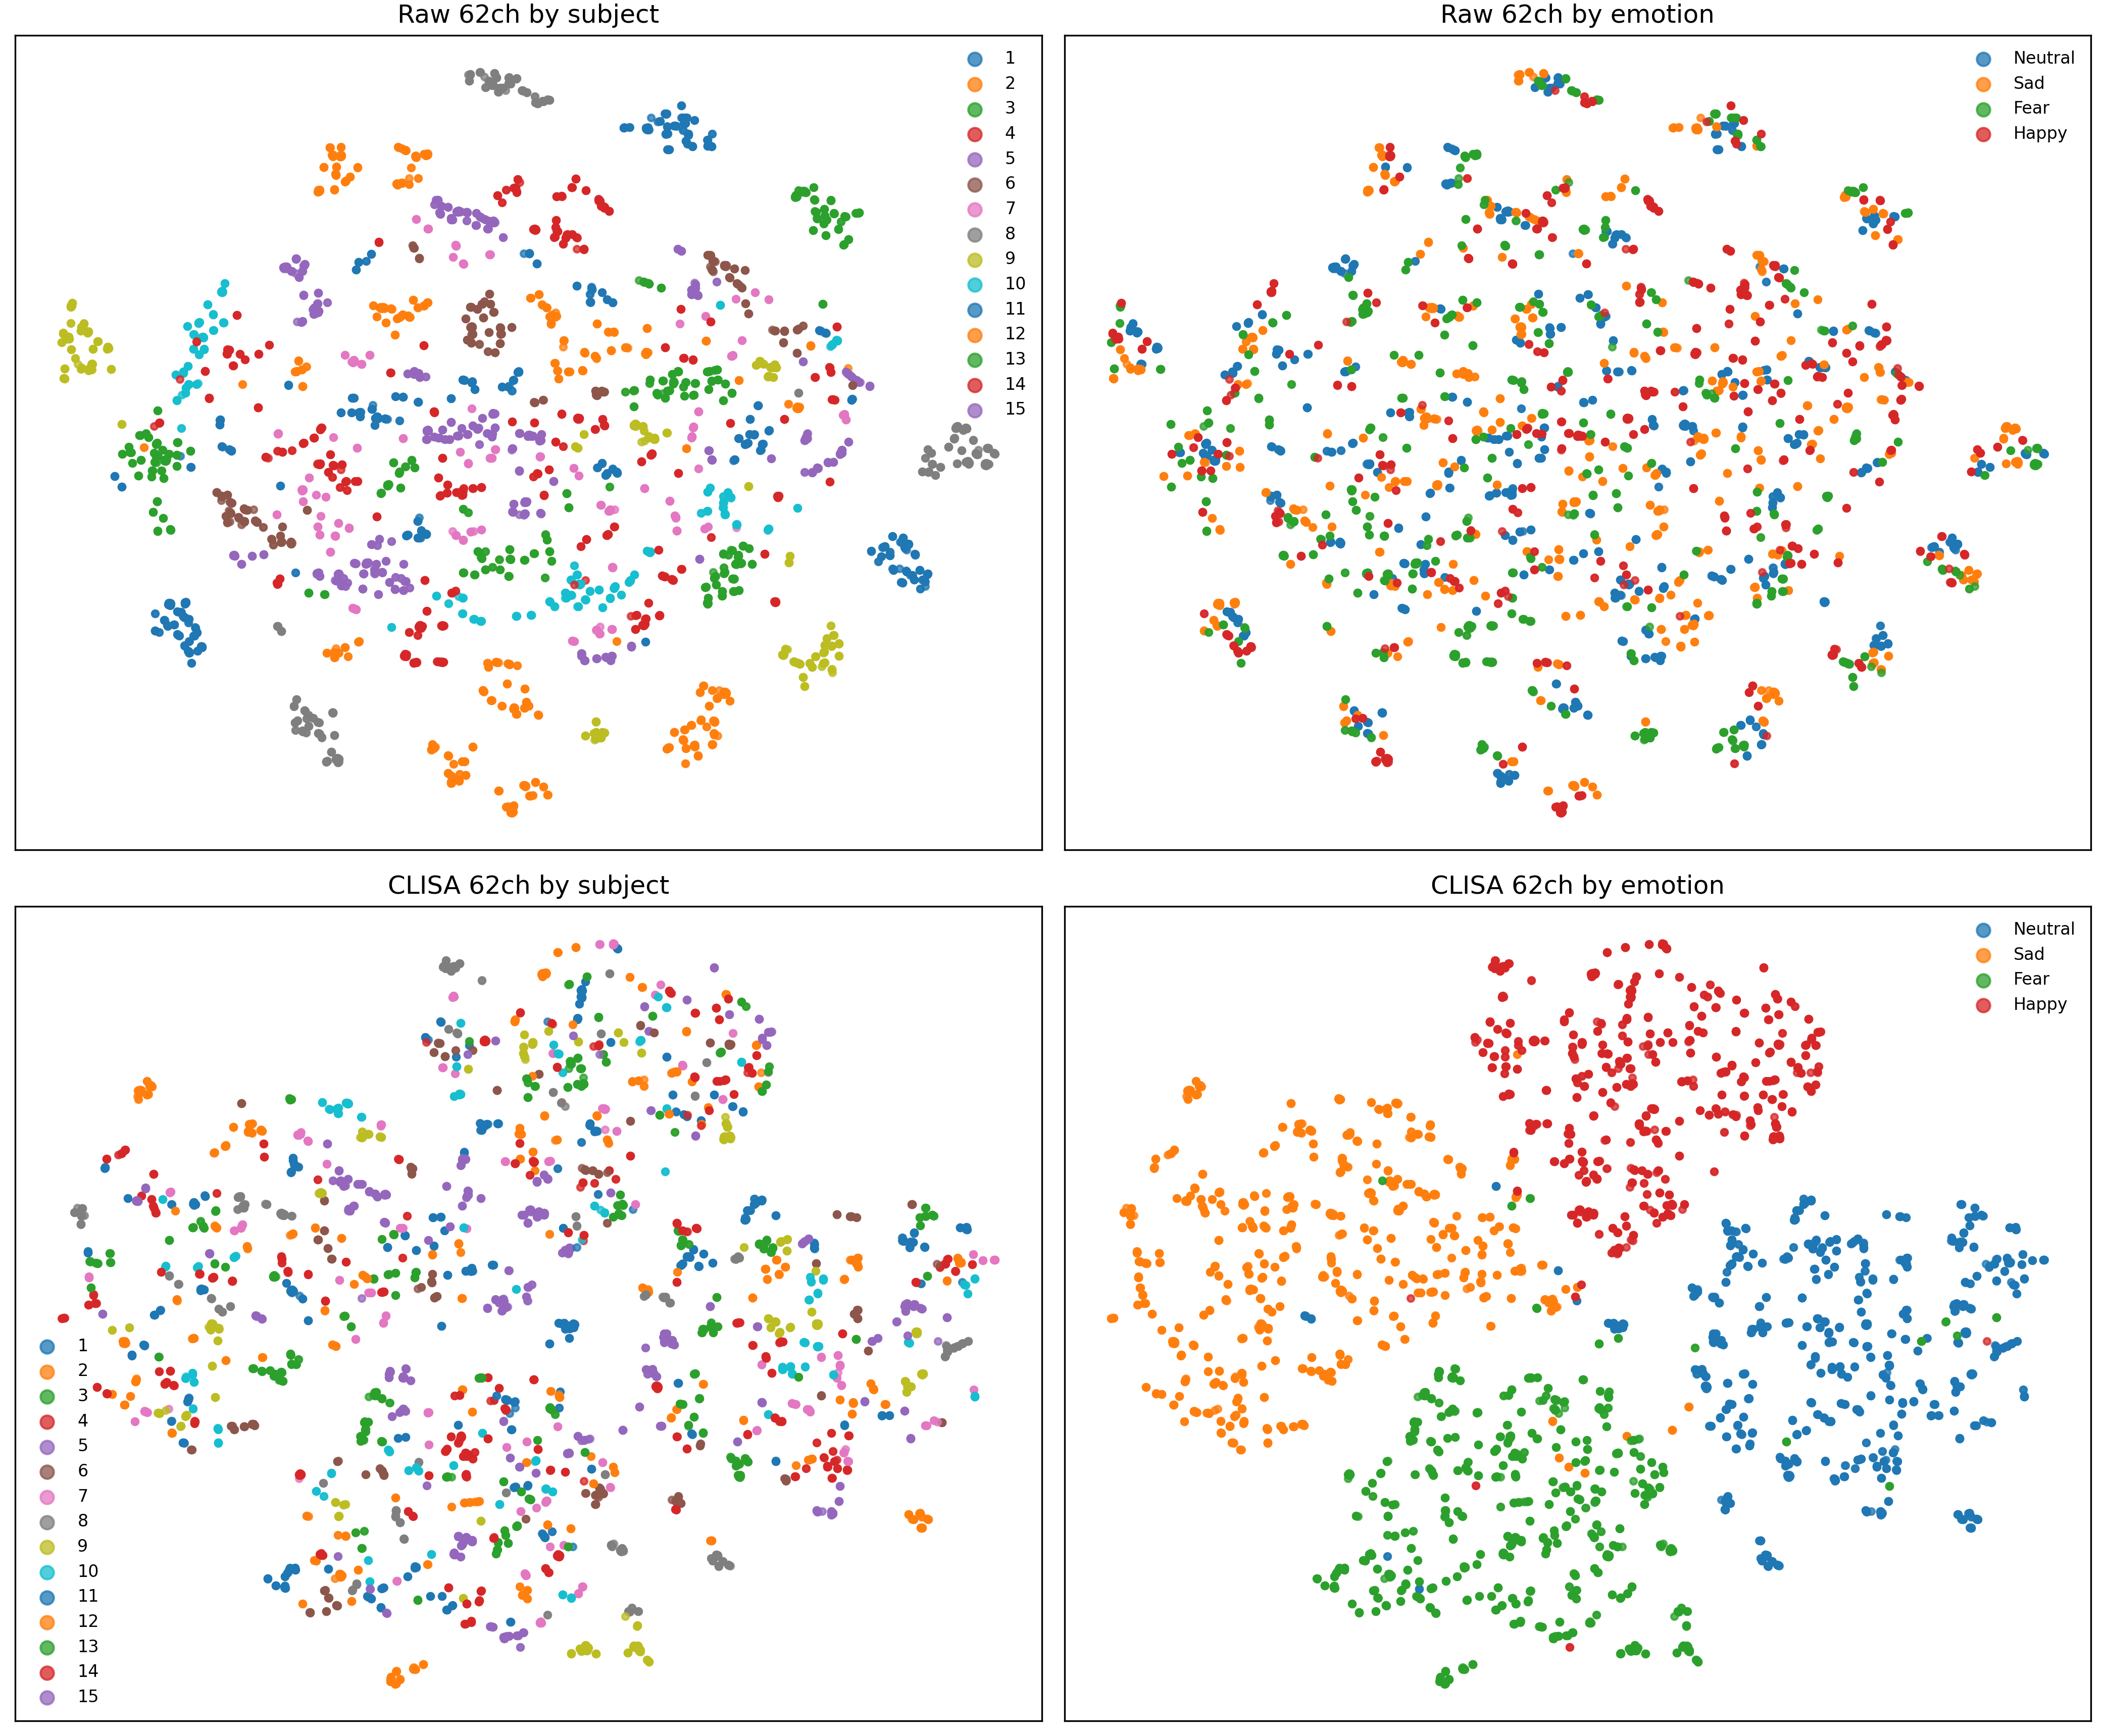
\includegraphics[width=1\linewidth,height=0.62\textheight,keepaspectratio]{figures/thesis_fig13_tsne_raw_vs_clisa.png}
  \caption{\textbf{Representation geometry.} t-SNE projections of raw 62-electrode differential-entropy features (top) and CLISA-EWU 62-electrode encoder embeddings (bottom), coloured by participant (left) and emotion (right). The embedding model is from the best run, and 14 of the 15 participants contributed labelled training data to it, so the emotion structure should be interpreted qualitatively.}
  \label{fig:tsne}
\end{figure}


\subsection{Secondary analyses}
The DANCE teacher–student pair was included as a secondary reference. Its calibrated accuracy was 0.519 (teacher, 62 electrodes) and 0.571 (student, six electrodes). An ablation of the DANCE framework is shown in Fig.~\ref{fig:abl}; four of its variants produced identical results, indicating that the corresponding options were not applied, so this ablation should be regarded as incomplete \pending{re-run, and add a CLISA-EWU ablation: no pretraining, noise-only, masking-only, temperature}. A software prototype, NeuroSync, displays signal traces, band power, predicted state and class probabilities from the trained model (Fig.~\ref{fig:neuro}); it was demonstrated on a synthetic replay session and has not been validated on live wearable recordings.

\begin{figure}[!htbp]
  \centering
  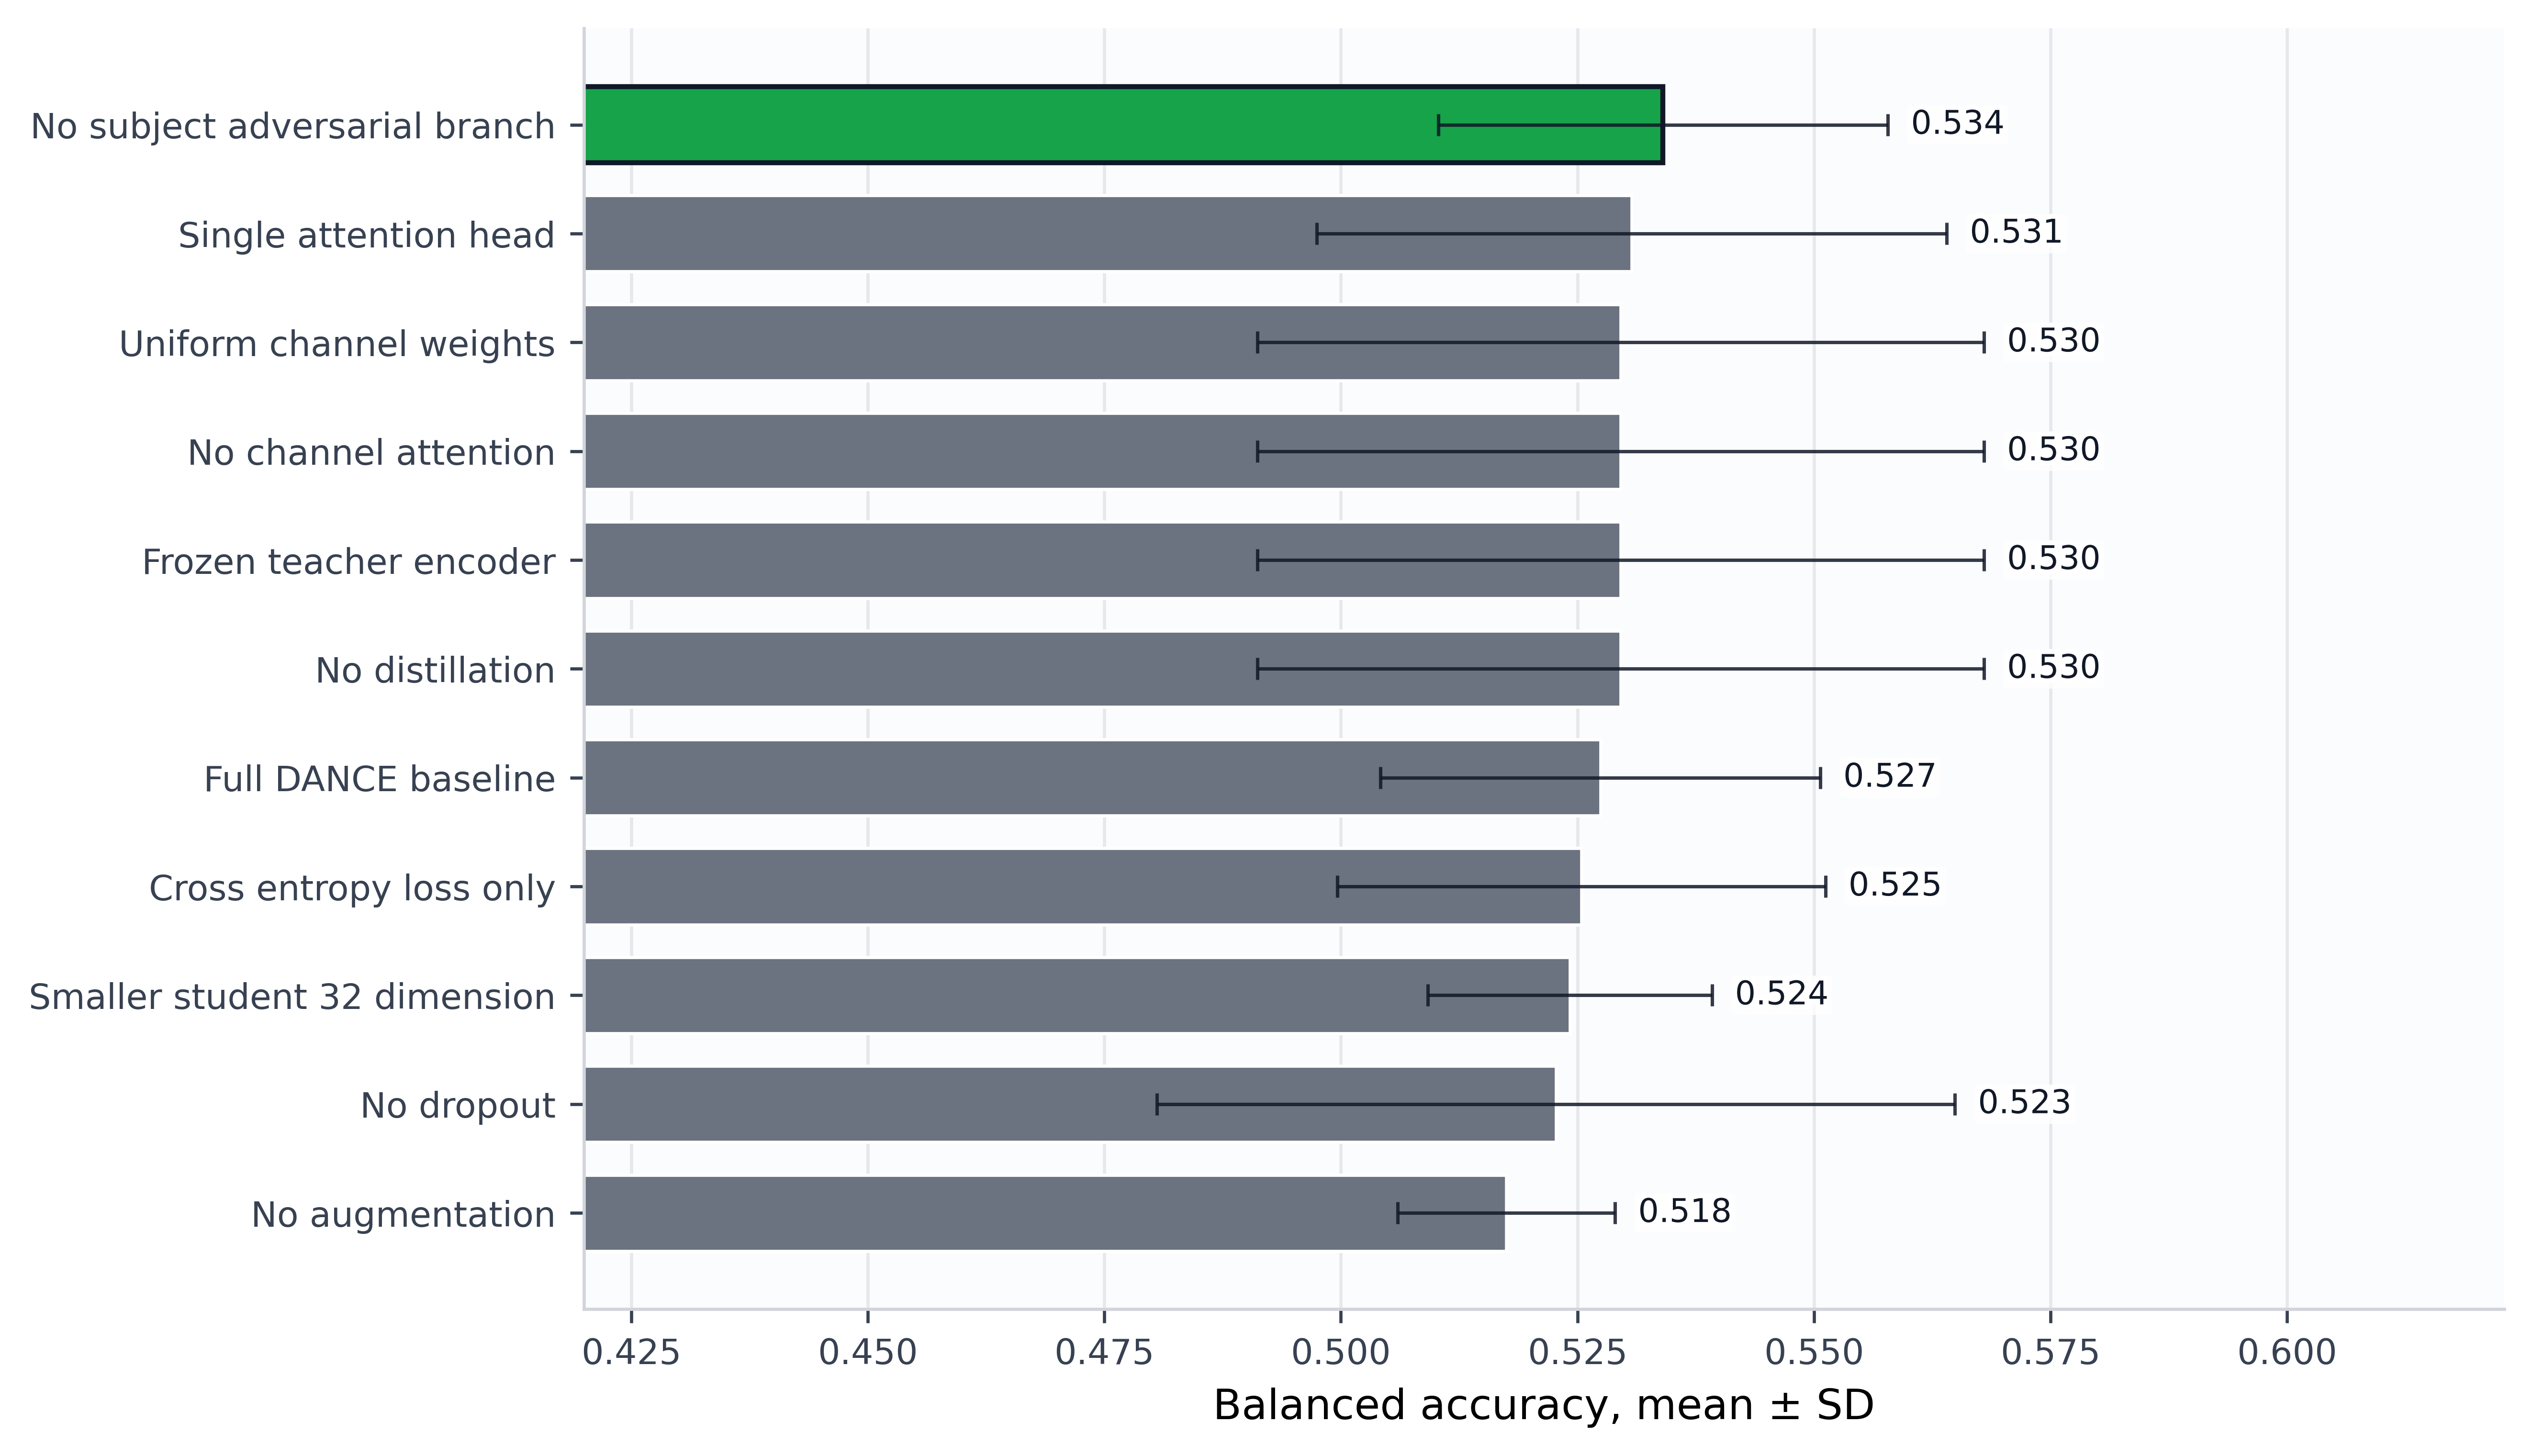
\includegraphics[width=1\linewidth,height=0.62\textheight,keepaspectratio]{figures/thesis_fig09_dance_ablation.png}
  \caption{\textbf{Ablation of the DANCE teacher–student framework (secondary comparator).} Calibrated accuracy (mean ± s.d. over three seeds) of 11 DANCE variants under a reduced protocol. Four variants produced identical values, indicating that their options were not applied; this ablation is incomplete and does not concern CLISA-EWU. The axis label ‘balanced accuracy’ in this thesis figure denotes accuracy (see Methods). \pending{Re-run before submission.}}
  \label{fig:abl}
\end{figure}

\begin{figure}[!htbp]
  \centering
  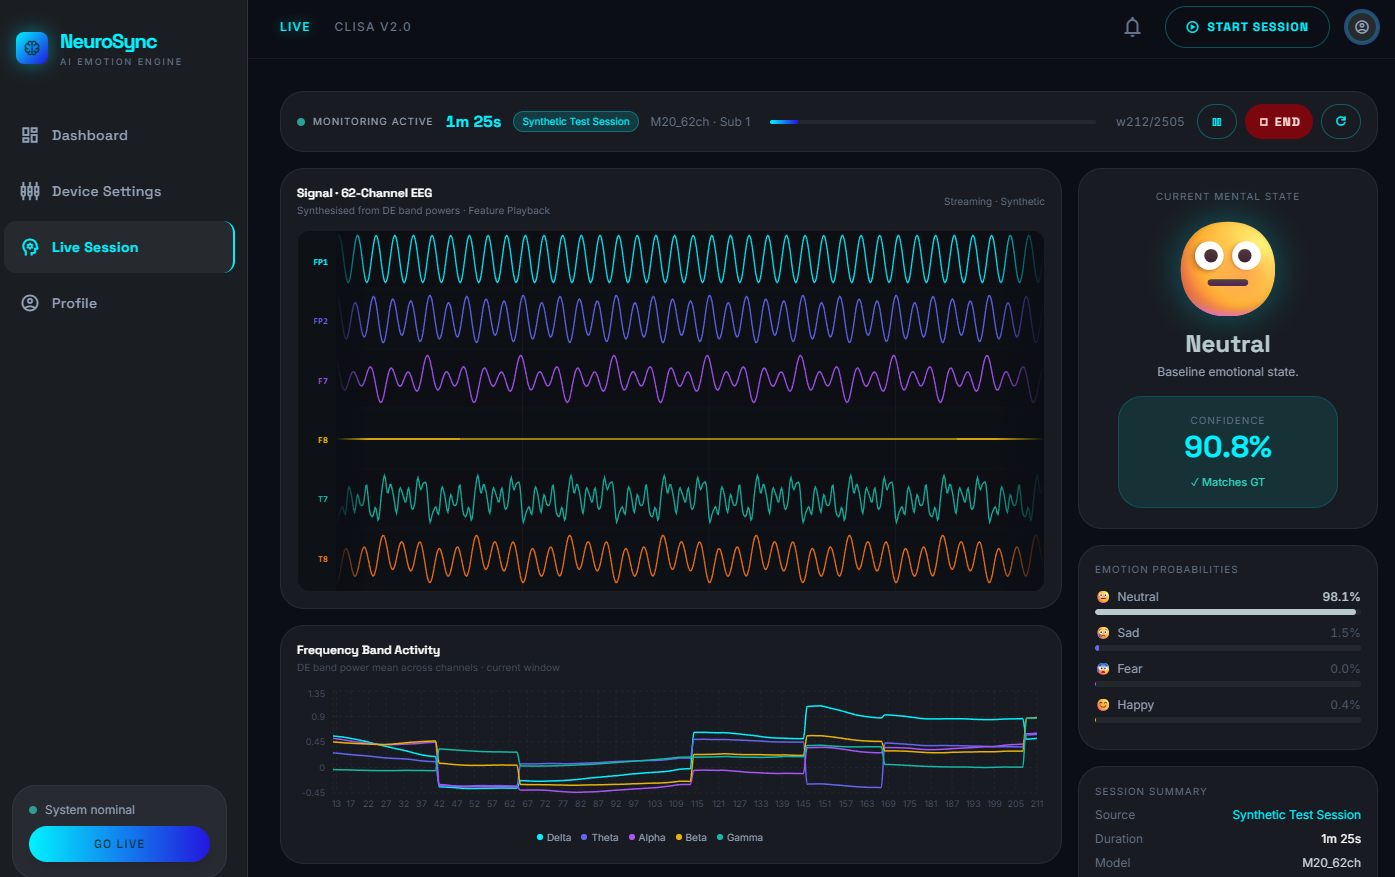
\includegraphics[width=1\linewidth,height=0.62\textheight,keepaspectratio]{figures/thesis_fig15_neurosync_dashboard.png}
  \caption{\textbf{NeuroSync dashboard prototype.} Signal traces, frequency-band activity, predicted state with confidence and class probabilities produced by the trained model during a synthetic replay session. Software demonstration only; not validated on live wearable recordings.}
  \label{fig:neuro}
\end{figure}


\subsection{Comparison with published studies}
The calibrated mean of CLISA-EWU (67.8\%) lies within the range of published cross-participant SEED-IV results (Table~\ref{tab:lit}), and the zero-shot mean (48.5\%) lies below it. Because the published values differ in their use of target-participant data and in reporting unit, they cannot be ranked against the present results; a fair comparison requires re-evaluating published architectures under both protocols used here.


\subsection{Implications}
These findings change how cross-participant results should be read. Much of the published progress on SEED-IV has been attributed to architectural innovation, yet our results suggest that the protocol, and specifically whether and how target-participant data are used, may explain as much variance as the architecture. Under calibration, the ordering of model families inverted: supervised networks that matched self-supervised models zero-shot fell far behind them. Comparisons that mix zero-shot, transductive and calibrated results, or that compare a best fold with another study's mean, are therefore uninterpretable. We recommend that cross-participant EEG studies report zero-shot and calibrated results separately, specify the number and selection of calibration samples, keep calibration and test trials disjoint, and summarise results at the participant level with confidence intervals\cite{tripod,kapoor}.

The practical message for wearable affective computing is cautiously positive. A short calibration session is acceptable in most consumer and research workflows, and a headband carrying frontal and temporal electrodes appears to keep most of the decodable signal under calibration. That some self-supervised models lost nothing from electrode reduction suggests that the frontal–temporal subset contains much of the information these models exploit, consistent with the established role of frontal activity in affect\cite{seed}. The attribution analysis indicates where the six-electrode montage falls short: fear relied on parieto-occipital electrodes outside the subset, and fear recall dropped most. A seven- or eight-electrode montage adding a parieto-occipital site is a natural next design to test. Nevertheless, the absolute calibrated accuracy (about 62\% for four classes with six electrodes) and the large between-participant spread mean that individual predictions remain unreliable, and the system is not suitable for clinical decisions.


\subsection{Limitations}
This study has limitations. The cohort was small (15 participants), healthy and drawn from one laboratory, and emotions were elicited with film clips under controlled conditions; generalisation to other populations, naturalistic settings and clinical groups is unknown \cite{seed,seedv,faced} \pending{external validation on SEED, SEED-V and FACED pending}. The six-electrode montage was simulated by selecting channels from a laboratory cap rather than recorded with a wearable device. Calibration windows were sampled across trials, so calibration and test windows could share a trial, which may have inflated calibrated accuracy\cite{liblock}. Labels were assigned per film clip rather than per moment. We used precomputed features, so preprocessing choices could not be varied, and hyperparameters were not tuned separately for each model. Finally, the contrastive model contrasted augmented views of single windows rather than aligning participants explicitly, so its gains should not be attributed to inter-participant alignment.


\section{Conclusion}
In this benchmark of 26 models under one leave-one-participant-out protocol, three findings stand out. First, decoding four emotions in an unseen participant without any of their data was modest for every model, and the deep architectures, including the contrastive model of primary interest, did not clearly outperform a two-layer perceptron. Second, about 80 s of labelled calibration data raised accuracy by roughly 20 percentage points, but only for models trained with contrastive, domain-adversarial or pseudo-label objectives. Third, a six-electrode frontal–temporal montage retained about nine-tenths of calibrated full-montage performance. In a controlled participant-independent benchmark, brief labelled calibration rather than architecture accounted for most of the measurable gain in EEG emotion recognition, and a six-electrode wearable-compatible montage retained about 91\% of calibrated performance. Rigorous separation of zero-shot and calibrated evaluation, external validation and real wearable recordings are the next steps towards dependable EEG-based affect sensing.


\section{Data availability}
The SEED-IV dataset is available from its providers under their licence at \url{https://bcmi.sjtu.edu.cn/home/seed/}. Data splits, per-fold predictions, confusion matrices and result tables are available at \url{https://github.com/saifkhancse/clisa-ewu-brain-informatics} \pending{archive a tagged release on Zenodo and cite its DOI}.

\section{Code availability}
Model, training, evaluation and analysis code, including the scripts that regenerate every statistic and figure in this paper, is available at \url{https://github.com/saifkhancse/clisa-ewu-brain-informatics}.

\begin{thebibliography}{99}
\bibitem{russell} Russell, J. A. A circumplex model of affect. J. Pers. Soc. Psychol. 39, 1161–1178 (1980).

\bibitem{seediv} Zheng, W.-L., Liu, W., Lu, Y., Lu, B.-L. \& Cichocki, A. EmotionMeter: a multimodal framework for recognizing human emotions. IEEE Trans. Cybern. 49, 1110–1122 (2019).

\bibitem{seed} Zheng, W.-L. \& Lu, B.-L. Investigating critical frequency bands and channels for EEG-based emotion recognition with deep neural networks. IEEE Trans. Auton. Ment. Dev. 7, 162–175 (2015).

\bibitem{deap} Koelstra, S. et al. DEAP: a database for emotion analysis using physiological signals. IEEE Trans. Affect. Comput. 3, 18–31 (2012).

\bibitem{clisa} Shen, X., Liu, X., Hu, X., Zhang, D. \& Song, S. Contrastive learning of subject-invariant EEG representations for cross-subject emotion recognition. IEEE Trans. Affect. Comput. https://doi.org/10.1109/TAFFC.2022.3164516 (2022). \pending{verify author list}

\bibitem{ganin} Ganin, Y. et al. Domain-adversarial training of neural networks. J. Mach. Learn. Res. 17, 1–35 (2016).

\bibitem{dan} Li, H., Jin, Y.-M., Zheng, W.-L. \& Lu, B.-L. Cross-subject emotion recognition using deep adaptation networks. In Neural Information Processing (ICONIP 2018) 403–413 (Springer, 2018).

\bibitem{bidann} Li, Y., Zheng, W., Cui, Z., Zhang, T. \& Zong, Y. A novel neural network model based on cerebral hemispheric asymmetry for EEG emotion recognition. In Proc. IJCAI 1561–1567 (2018).

\bibitem{bihdm} Li, Y. et al. A novel bi-hemispheric discrepancy model for EEG emotion recognition. IEEE Trans. Cogn. Dev. Syst. 13, 354–367 (2021).

\bibitem{dgcnn} Song, T., Zheng, W., Song, P. \& Cui, Z. EEG emotion recognition using dynamical graph convolutional neural networks. IEEE Trans. Affect. Comput. 11, 532–541 (2020).

\bibitem{rgnn} Zhong, P., Wang, D. \& Miao, C. EEG-based emotion recognition using regularized graph neural networks. IEEE Trans. Affect. Comput. 13, 1290–1301 (2022).

\bibitem{sognn} Li, J., Li, S., Pan, J. \& Wang, F. Cross-subject EEG emotion recognition with self-organized graph neural network. Front. Neurosci. 15, 611653 (2021).

\bibitem{bfenet} Zhang, J. et al. Subject-independent emotion recognition based on EEG frequency band features and self-adaptive graph construction. Brain Sci. 14, 271 (2024).

\bibitem{attgraph} Zhang, S., Chu, C., Zhang, X. \& Zhang, X. EEG emotion recognition using AttGraph: a multi-dimensional attention-based dynamic graph convolutional network. Brain Sci. 15, 615 (2025).

\bibitem{ssemerge} Ahuja, C. \& Sethia, D. SS-EMERGE: self-supervised enhancement for multidimension emotion recognition using GNNs for EEG. Sci. Rep. 15, 14254 (2025).

\bibitem{saeb} Saeb, S., Lonini, L., Jayaraman, A., Mohr, D. C. \& Kording, K. P. The need to approximate the use-case in clinical machine learning. GigaScience 6, 1–9 (2017).

\bibitem{kapoor} Kapoor, S. \& Narayanan, A. Leakage and the reproducibility crisis in machine-learning-based science. Patterns 4, 100804 (2023).

\bibitem{liblock} Li, R. et al. The perils and pitfalls of block design for EEG classification experiments. IEEE Trans. Pattern Anal. Mach. Intell. 43, 316–333 (2021).

\bibitem{simclr} Chen, T., Kornblith, S., Norouzi, M. \& Hinton, G. A simple framework for contrastive learning of visual representations. In Proc. ICML 1597–1607 (2020).

\bibitem{byol} Grill, J.-B. et al. Bootstrap your own latent: a new approach to self-supervised learning. Adv. Neural Inf. Process. Syst. 33, 21271–21284 (2020).

\bibitem{pseudo} Lee, D.-H. Pseudo-label: the simple and efficient semi-supervised learning method for deep neural networks. In ICML Workshop on Challenges in Representation Learning (2013).

\bibitem{mixmatch} Berthelot, D. et al. MixMatch: a holistic approach to semi-supervised learning. Adv. Neural Inf. Process. Syst. 32 (2019).

\bibitem{hinton} Hinton, G., Vinyals, O. \& Dean, J. Distilling the knowledge in a neural network. Preprint at https://arxiv.org/abs/1503.02531 (2015).

\bibitem{xgboost} Chen, T. \& Guestrin, C. XGBoost: a scalable tree boosting system. In Proc. 22nd ACM SIGKDD 785–794 (2016).

\bibitem{vaswani} Vaswani, A. et al. Attention is all you need. Adv. Neural Inf. Process. Syst. 30 (2017).

\bibitem{conformer} Song, Y., Zheng, Q., Liu, B. \& Gao, X. EEG Conformer: convolutional transformer for EEG decoding and visualization. IEEE Trans. Neural Syst. Rehabil. Eng. 31, 710–719 (2023).

\bibitem{brodersen} Brodersen, K. H., Ong, C. S., Stephan, K. E. \& Buhmann, J. M. The balanced accuracy and its posterior distribution. In Proc. 20th Int. Conf. Pattern Recognit. 3121–3124 (2010).

\bibitem{cohen} Cohen, J. A coefficient of agreement for nominal scales. Educ. Psychol. Meas. 20, 37–46 (1960).

\bibitem{gorodkin} Gorodkin, J. Comparing two K-category assignments by a K-category correlation coefficient. Comput. Biol. Chem. 28, 367–374 (2004).

\bibitem{chicco} Chicco, D. \& Jurman, G. The advantages of the Matthews correlation coefficient (MCC) over F1 score and accuracy in binary classification evaluation. BMC Genomics 21, 6 (2020).

\bibitem{kubat} Kubat, M. \& Matwin, S. Addressing the curse of imbalanced training sets: one-sided selection. In Proc. 14th Int. Conf. Mach. Learn. 179–186 (1997).

\bibitem{wolpaw} Wolpaw, J. R., Birbaumer, N., McFarland, D. J., Pfurtscheller, G. \& Vaughan, T. M. Brain–computer interfaces for communication and control. Clin. Neurophysiol. 113, 767–791 (2002).

\bibitem{friedman} Friedman, M. The use of ranks to avoid the assumption of normality implicit in the analysis of variance. J. Am. Stat. Assoc. 32, 675–701 (1937).

\bibitem{demsar} Demšar, J. Statistical comparisons of classifiers over multiple data sets. J. Mach. Learn. Res. 7, 1–30 (2006).

\bibitem{wilcoxon} Wilcoxon, F. Individual comparisons by ranking methods. Biom. Bull. 1, 80–83 (1945).

\bibitem{holm} Holm, S. A simple sequentially rejective multiple test procedure. Scand. J. Stat. 6, 65–70 (1979).

\bibitem{lakens} Lakens, D. Calculating and reporting effect sizes to facilitate cumulative science: a practical primer for t-tests and ANOVAs. Front. Psychol. 4, 863 (2013).

\bibitem{kerby} Kerby, D. S. The simple difference formula: an approach to teaching nonparametric correlation. Compr. Psychol. 3, 11.IT.3.1 (2014).

\bibitem{shrout} Shrout, P. E. \& Fleiss, J. L. Intraclass correlations: uses in assessing rater reliability. Psychol. Bull. 86, 420–428 (1979).

\bibitem{tripod} Collins, G. S. et al. TRIPOD+AI statement: updated guidance for reporting clinical prediction models that use regression or machine learning methods. BMJ 385, e078378 (2024).

\bibitem{tsne} van der Maaten, L. \& Hinton, G. Visualizing data using t-SNE. J. Mach. Learn. Res. 9, 2579–2605 (2008).

\bibitem{silhouette} Rousseeuw, P. J. Silhouettes: a graphical aid to the interpretation and validation of cluster analysis. J. Comput. Appl. Math. 20, 53–65 (1987).

\bibitem{dbi} Davies, D. L. \& Bouldin, D. W. A cluster separation measure. IEEE Trans. Pattern Anal. Mach. Intell. 1, 224–227 (1979).

\bibitem{chi} Caliński, T. \& Harabasz, J. A dendrite method for cluster analysis. Commun. Stat. 3, 1–27 (1974).

\bibitem{shap} Lundberg, S. M. \& Lee, S.-I. A unified approach to interpreting model predictions. Adv. Neural Inf. Process. Syst. 30 (2017).

\bibitem{adabn} Li, Y., Wang, N., Shi, J., Hou, X. \& Liu, J. Adaptive batch normalization for practical domain adaptation. Pattern Recognit. 80, 109–117 (2018).

\bibitem{landis} Landis, J. R. \& Koch, G. G. The measurement of observer agreement for categorical data. Biometrics 33, 159–174 (1977).

\bibitem{seedv} Liu, W., Qiu, J.-L., Zheng, W.-L. \& Lu, B.-L. Comparing recognition performance and robustness of multimodal deep learning models for multimodal emotion recognition. IEEE Trans. Cogn. Dev. Syst. 14, 715–729 (2022).

\bibitem{faced} Chen, J. et al. A large finer-grained affective computing EEG dataset. Sci. Data 10, 740 (2023).
\end{thebibliography}

\section*{Acknowledgements}
The authors thank the providers of the SEED-IV dataset and the Department of Computer Science and Engineering, East West University, for their support. All figures were created by the authors; schematic illustrations (Figs.~\ref{fig:workflow} and \ref{fig:arch}) were drawn manually and all plots were generated with Python.

\section*{Author contributions}
S.K.: conceptualization, methodology, software, experiments, formal analysis, visualization and writing of the original draft. O.B.Q.: experiments, analysis and manuscript preparation. K.M.F.A.B.: implementation, evaluation and documentation. R.R.: experiments, reporting and software integration (NeuroSync). A.W.R.: supervision, review and editing. All authors reviewed and approved the final manuscript.

\section*{Funding}
No external funding was received for this study \pending{confirm}.

\section*{Declarations}
\subsection*{Competing interests}
The authors declare no competing interests.

\subsection*{Additional information}
\textbf{Correspondence} and requests for materials should be addressed to S.K.

\end{document}
